% Format teze zasnovan je na paketu memoir
% http://tug.ctan.org/macros/latex/contrib/memoir/memman.pdf ili
% http://texdoc.net/texmf-dist/doc/latex/memoir/memman.pdf
% 
% Prilikom zadavanja klase memoir, navedenim opcijama se podešava 
% veličina slova (12pt) i jednostrano štampanje (oneside).
% Ove parametre možete menjati samo ako pravite nezvanične verzije
% mastera za privatnu upotrebu (na primer, u b5 varijanti ima smisla 
% smanjiti 
\documentclass[12pt,oneside]{memoir} 




% Paket koji definiše sve specifičnosti master rada Matematičkog fakulteta
\usepackage[latinica]{matfmaster} 
%
% Podrazumevano pismo je ćirilica.
%   Ako koristite pdflatex, a ne xetex, sav latinički tekst na srpskom jeziku
%   treba biti okružen sa \lat{...} ili \begin{latinica}...\end{latinica}.
%
% Opicija [latinica]:
%   ako želite da pišete latiniciom, dodajte opciju "latinica" tj.
%   prethodni paket uključite pomoću: \usepackage[latinica]{matfmaster}.
%   Ako koristite pdflatex, a ne xetex, sav ćirilički tekst treba biti
%   okružen sa \cir{...} ili \begin{cirilica}...\end{cirilica}.
%
% Opcija [biblatex]:
%   ako želite da koristite reference na više jezika i umesto paketa
%   bibtex da koristite BibLaTeX/Biber, dodajte opciju "biblatex" tj.
%   prethodni paket uključite pomoću: \usepackage[biblatex]{matfmaster}
%
% Opcija [b5paper]:
%   ako želite da napravite verziju teze u manjem (b5) formatu, navedite
%   opciju "b5paper", tj. prethodni paket uključite pomoću: 
%   \usepackage[b5paper]{matfmaster}. Tada ima smisla razmisliti o promeni
%   veličine slova (izmenom opcije 12pt na 11pt u \documentclass{memoir}).
%
% Naravno, opcije je moguće kombinovati.
% Npr. \usepackage[b5paper,biblatex]{matfmaster}







% Datoteka sa literaturom u BibTex tj. BibLaTeX/Biber formatu
\bib{marina-master}

% Ime kandidata na srpskom jeziku (u odabranom pismu)
\autor{Marina R. Nikolić}
% Naslov teze na srpskom jeziku (u odabranom pismu)
\naslov{Prikupljanje i prikaz podataka o izvršavanju programa}
% Godina u kojoj je teza predana komisiji
\godina{2018}
% Ime i afilijacija mentora (u odabranom pismu)
\mentor{dr Milena \textsc{Vujošević Janičić}, docent\\ Univerzitet u Beogradu, Matematički fakultet}
% Ime i afilijacija prvog člana komisije (u odabranom pismu)
\komisijaA{dr Filip \textsc{Marić}, vanredni profesor\\ Univerzitet u Beogradu, Matematički fakultet}
% Ime i afilijacija drugog člana komisije (u odabranom pismu)
\komisijaB{dr Milan \textsc{Banković}, docent\\ Univerzitet u Beogradu, Matematički fakultet}
% Ime i afilijacija trećeg člana komisije (opciono)
% \komisijaC{}
% Ime i afilijacija četvrtog člana komisije (opciono)
% \komisijaD{}
% Datum odbrane (odkomentarisati narednu liniju i upisati datum odbrane ako je poznat)
% \datumodbrane{}

% Apstrakt na srpskom jeziku (u odabranom pismu)
\apstr{tekst apstrakta rada
}

% Ključne reči na srpskom jeziku (u odabranom pismu)
\kljucnereci{profajliranje, pokrivenost koda, GCC, GCOV}


% Komande za naglašavanje
\newcommand{\kod}[1]{\texttt{#1}}
\newcommand{\strano}[1]{\textit{#1}}

%Listing podesavanja za kod
\usepackage{listings}
\definecolor{mygreen}{rgb}{0,0.6,0}
\definecolor{mygray}{rgb}{0.5,0.5,0.5}
\definecolor{mymauve}{rgb}{0.58,0,0.82}
\lstset{ 
  backgroundcolor=\color{white},   % choose the background color; you must add \usepackage{color} or \usepackage{xcolor}; should come as last argument
  basicstyle=\scriptsize\ttfamily,        % the size of the fonts that are used for the code
  breakatwhitespace=false,         % sets if automatic breaks should only happen at whitespace
  breaklines=true,                 % sets automatic line breaking
  captionpos=b,                    % sets the caption-position to bottom
  commentstyle=\color{mygreen},    % comment style
  deletekeywords={...},            % if you want to delete keywords from the given language
  escapeinside={\%*}{*)},          % if you want to add LaTeX within your code
  extendedchars=true,              % lets you use non-ASCII characters; for 8-bits encodings only, does not work with UTF-8
  firstnumber=1000,                % start line enumeration with line 1000
  frame=single,	                   % adds a frame around the code
  keepspaces=true,                 % keeps spaces in text, useful for keeping indentation of code (possibly needs columns=flexible)
  keywordstyle=\color{blue},       % keyword style
  language=C,                 % the language of the code
  morekeywords={*,...},            % if you want to add more keywords to the set
  numbers=left,                    % where to put the line-numbers; possible values are (none, left, right)
  numbersep=5pt,                   % how far the line-numbers are from the code
  numberstyle=\tiny\color{mygray}, % the style that is used for the line-numbers
  rulecolor=\color{black},         % if not set, the frame-color may be changed on line-breaks within not-black text (e.g. comments (green here))
  showspaces=false,                % show spaces everywhere adding particular underscores; it overrides 'showstringspaces'
  showstringspaces=false,          % underline spaces within strings only
  showtabs=false,                  % show tabs within strings adding particular underscores
  stepnumber=2,                    % the step between two line-numbers. If it's 1, each line will be numbered
  stringstyle=\color{mymauve},     % string literal style
  tabsize=2,	                   % sets default tabsize to 2 spaces
  title=\lstname                   % show the filename of files included with \lstinputlisting; also try caption instead of title
}


\begin{document}
% ==============================================================================
% Uvodni deo teze
\frontmatter
% ==============================================================================
% Naslovna strana
\naslovna
% Strana sa podacima o mentoru i članovima komisije
\komisija
% Strana sa posvetom (u odabranom pismu)
\posveta{Mentoru za predanost i pomoć, firmi za resurse, porodici i prijateljima za podršku}
% Strana sa podacima o disertaciji na srpskom jeziku
\apstrakt
% Sadržaj teze
\tableofcontents

% ==============================================================================
% Glavni deo teze
\mainmatter
% ==============================================================================

% ------------------------------------------------------------------------------
\chapter{Uvod}
% ------------------------------------------------------------------------------

Razvoj komercionalnog softvera, za koji su standardi kvaliteta u pogledu korektnosti, performansi i upotrebljivosti vrlo visoki, mora sadržati i napredne i iscrpne faze testiranja i optimizacije. Spovođenje ovih faza, na način koji svojom brzinom i efikasnošću garantuje kompetentnost na današnjem tržištu, uslovljeno je dobrim poznavanjem koda softvera, pre svega ponašanja u različitim slučajevima upotrebe, kritičnih sekcija, memorijski ili vremenski zahtevnih segmenata i slično. Kompleksnost funkcionalnih zahteva  klijenata, ograničene hardverske mogućnosti kao i visoka tranzitivnost stručnog kadra, samo su neki od faktora koji utiču na smanjenje nivoa poznavanja interne strukture i ponašanja, čime u velikoj meri otežavaju procese testiranja i optimizacije.

Nadoknađivanje nedostajućeg znanja, može se postići primenom određenih tehnika dinamičke analize programa, kao što je profajliranje. Instrumentalizacijom koda se u njega ugrađuju posebne instrukcije za praćenje izvršavanja, zahvaljujući kojima alati za profajliranje prikupljaju sirove metapodatke koje će dalje preraditi u korisne informacije, poput pokrivenosti, odnosno stepena izvršenosti, celokupnog koda ili neke njegove celine. One obezbeđuju potrebno znanje o tokovima izvršavanja u različitim slučajevima upotrebe, ali i o opterećnosti konkretnih segmenata rada programa. Zbog toga predstavljaju važnu smernicu razvojnom timu u procesima testiranja i optimizacije.

Većina poznatijih prevodioca, poput \strano{GCC}-a \cite{GCC}, \strano{ICC}-a \cite{ICC} ili \strano{Clang}-a \cite{CLANG} sadrže u sebi ugrađenu podršku za prikupljanje podataka iz izvršavanja, kao i alate za njihovu obradu i prevođenje u format pogodan za čitanje i analiziranje od strane razvojnog tima. Zahvaljujući svojim performasama, odnosno boljoj vremenskoj i prostornoj složenosti u odnosu na profajliranje alatima \strano{Clang}-a, kao i dostupnosti koda i besplatnim korišćenjem, kojom prednjači u odnosu na \strano{ICC}, ističe se programski prevodilac \strano{GCC} sa svojim alatom \strano{gcov} \cite{GCOV}. Izveštaji kreirani ovim alatom sadrže veoma korisne informacije o izvršenosti pojedinačnih linija, funkcija, blokova ili grana. 

Međutim, pored izuzetnih performansi, trenutna implementacija prikupljanja podataka iz izvršavanja u okviru \strano{GCC}-a, poseduje i jedan važan nedostatak u odnosu na \strano{Clang}, a to je nedostupnost tih podataka pre završetka rada analiziranog programa. U specifičnim situacijama, kada je izvršavanje isuviše dugo i/ili se ne sme prekidati zbog profajliranja, potrebno je obezbediti ove informacije u toku rada programa.
 
Iz tih razloga je, u okviru ovog rada, implementirana podrška za prikupljanje podataka iz izvršavanja u toku rada programa, proširivanjem mogućnosti programskog prevodioca \strano{GCC}. Pored toga, kreiran je i novi grafički interfejs za prikaz tih podataka, koji nadomešćuje nedostatke alata \strano{gcov} u pogledu preglednosti, informativnosti na nivou većem od pojedinačnog fajla izvornog koda, kao i ukupnog kvaliteta korisničkog doživljaja. Testiranje implementiranog rešenja sprovedeno je nad kompleksnim softverom koji služi za emuliranje različitih arhitektura, pod nazivom \strano{QEMU} \cite{QEMU}. 

Drugo poglavlje rada predstavlja uvod u analizu programa, njene vrste i tehnike. Posebna pažnja posvećena je tehnici dinamičke analize pod nazivom profajliranje, koja obuhvata proces instrumentalizacije koda, prikupljanja i obrade podataka iz izvršavanja programa. Definisani su i pojam i značaj pokrivenosti koda, kao jedne od najvažnijih informacija koja se izvodi iz tih podataka. Počevši od narednog poglavlja vrši se restrikcija na programski prevodilac \strano{GCC}. U okviru trećeg poglavlja, opisana je detaljno postojeća implementacija prikupljanja podataka i demonstrirarane mogućnosti alata \strano{gcov}, dok se u okviru četvrtog poglavlja nalaze detalji implementacije unapređenja koje predstavlja osnovu ovog rada: proširenje mogućnosti programskog prevodioca \strano{GCC} u cilju dobijanja podataka iz izvršavanja pre kraja programa i kreiranje novog grafičkog interfejsa za njihov prikaz. Peto poglavlje posvećeno je procesima testiranja i analize performansi, najpre nad jednim jednostavnijim primerom, a zatim i nad alatom \strano{QEMU}.

% ------------------------------------------------------------------------------
\chapter{Analiza performansi programa}
% ------------------------------------------------------------------------------


Razvoj softvera je znatno širi pojam od pisanja koda. Obuhvata više, podjednako važnih segmenata, kao što su: planiranje, analiza i usklađivanje sa zahtevima klijenata, testiranje, analiza performansi, optimizacija ili održavanje. Samo investiranjem u svaki ponaosob, može se proizvesti kvalitetan i dugotrajan softver. Njihova kompleksnost proporcijano raste sa značajem i složenošću krajnjeg proizvoda, iz čega proističe i važnost njihovog olakšavanja. Postoje brojne metodologije i tehnike koje su specijalizovane za vođenje procesa karakterističnih za rane faze razvoja, kao što su planiranja ili analize zahteva. Međutim, ovaj rad će se usresrediti na prikaz onih koje olakšavaju procese kasnog razvoja, pre svega testiranja i optimizacije. Za uspešno sprovođenje tih procesa, važan faktor je odabir tehnika koje će se primenjivati i jedinica koda kome su oni najneophodniji, a kvalitetan odabir je uslovljen dobrim poznavanjem samog softvera, njegovih karakteristika i ponašanja. Takvu vrstu informacije obezbeđuje analiza programa.

\section{Vrste analize programa}

U okviru analize programa razmatraju se razni aspekti softvera, pre svega, aspekti ponašanja softvera u različitim sučajevima upotrebe. Analiza softvera može da bude automatizovana i u nastavku teksta biće razmatrani koncepti koji su vezani za automatizovane pristupe. Cilj analize je olakšavanje procesa testiranja korektnosti, naročito eksterno nabavljenih delova softvera kao i procene performansi i optimizacije. Analiza treba da pruži korisne informacije o raspodeli potrošnje resursa, čvorovima ekstremne potrošnje, potencijalnim kritičnim segmentima izvršavanja, korektnosti toka izvršavanja i slično. Poput projekta veštačke inteligencije, njen krajnji cilj je stvaranje "pametnog prevodioca", koji bi mogao automatski generisati efikasan, a pouzdan k\^{o}d. Značaj njenih trenutnih mogućnosti, kao i brzina kojom se unapređuje, ukazuju na veliku verovatnoću ostvarljivosti tog cilja. Analiza programa je veoma širok pojam, koji obuhvata veliki broj vrlo raznovrsnih metoda, ali se može veoma precizno podeliti na dva osnovna tipa. To su statička i dinamička analiza.

\subsection{Statička analiza programa}

Statička analiza programa \cite{Static} obuhvata sve metode i tehnike utvrđivanja ponašanja programa, za koje ga nije potrebno izvršiti. Sve procedure se vrše nad izvornim kodom i, prikupljajući podatke o njegovoj strukturi, generišu korisne informacije o mogućim ishodima njegovog budućeg izvršavanja. Primer su mnogobrojne softverske metrike, koje na osnovu podataka o broju linija, klasa ili metoda, izračunavaju takozvani "statistički kvalitet" softvera. 

Njena glavna prednost proističe upravo iz toga, što k\^{o}d nije potrebno izvršiti. Ovakvim ograničenjem se često odlikuje razvoj velikih i skupih softverskih sistema, gde se zbog materijalnih mogućnosti ne može vršiti testiranje svih manjih jedinica u realnom okruženju. Kao ilustrativan primer se može posmatrati razvoj softera za automatsko navođenje rakete i jedan manji segment tog razvoja koji predstavlja program za izračunavanje potrošnje goriva prilikom jednje vožnje. Testiranje korektnosti sastavne jedinice te veličine se u najvećoj meri vrši na simulatorima. Lansiranje prave rakete za potrebe ovakvog testiranja je ekonomski neopravdano, iako okruženje koje simulator pruža ne obuhvata sve alternativne slučajeve upotrebe. 

Sa druge strane, ukoliko uzmemo u obzir činjenicu da vreme izvršavanja proizvoljnog programa može biti proizvoljno dugo, iz neneophodnosti izvršavanja, može se izvesti još jedna velika prednost statičke analize, a to je brzina. Faktor brzine čini osnovu ocene svakog pristupa.

Statička analiza programa se ne bazira na podacima iz konkretnih izvršavanja, već nepromenljivim i sigurnim podacima izvornog koda, zbog čega je odlikuje i nepristrasnost. Nezavisnost od ulaznih podataka i okruženja, omogućava efikasnu detekciju graničnih slučajeva.
 
Osnovne mane softverskih metrika su uzrokovane uskom vezom njihovih tehnika sa statistikom kao naukom i predstavljaju nepreciznost i smanjenu informativnost o praktičnim slučajevima upotrebe. Rezultati nisu eksperimentalne prirode, već prikazuju teorijsko predviđanje ponašanja. Zbog toga se ne trebaju smatrati potvrdama ispravnosti ili performansi, već isključivo tretirati kao smernice pri razvoju.

Postoje i određene statičke metode koje su značajno preciznije od metrika, poput simboličkog izvršavanja \cite{Simbolicko}, proveravanja modela \cite{TestModel} ili apstraktne interpretacije \cite{Apstraktno}. Ove metode simuliraju ponašanje programa uzimajući u obzir i ulazne vrednosti, čime se povećava preciznost i informativnost. Međutim, uticaj realnih parametara okruženja, čija specifikacija nije u potpunosti poznata, se i dalje zasniva na predviđanju i statističkim informacijama o slučajevima upotrebe. Kao primer nedovoljeno potpune specifikacije se mogu posmatrati eksterno nabavljene komponente sa zatvorenim kodom. Nepoznavanje svih alternativnih tokova upotrebe ili greške u dokumentaciji mogu prouzrokovati slabosti u modelima kreiranim ovim metodama.

\subsection{Dinamička analiza programa}

Dinamička analiza programa \cite{Gupta} obuhvata sve metode i tehnike prikupljanja podataka o programu tokom njegovog izvršavanja i utvrđivanja ponašanja programa na osnovu tih podataka. Procedure uglavnom započinju u fazi prevođenja, ali najvažniji deo se obavlja u toku i nakon izvršavanja. Pored strukture koda i statičkih podataka, na njen ishod utiču i ulazne vrednosti, kao i parametri okruženja. Testovi jedinica koda, sistemski testovi i testovi prihvatljivosti koriste isključivo ovaj vid analize programa. 

Sve njene glavne prednosti u odnosu na statičku analizu, proističu iz uticaja "realnih parametara". Određene mane softverskih rešenja ispoljavaju se samo u toku rada tog softvera, a mnoge i proističu upravo iz spoljnih faktora ili veze sa njima. Statistički savršen softver koji je nedovoljno primenljiv u praksi, predstavlja jedan od tri osnovna neuspeha prilikom razvoja softvera \cite{Malkov}. Marketinška istraživanja, analize zahteva korisnika i detaljni popisi slučajeva upotrebe se primenjuju u ranim fazama razvoja softvera u cilju zaštite od ove vrste neuspeha. Međutim, pojedini faktori okruženja, poput vrednosti jedne jedinice iz skupa obrade, čiji uticaj se zanemaruje kao dozvoljeno odstupanje, greška zaokruživanja ili usled efekta mase, tzv. "lažne pozitivne ili negativne vrednosti", se ne mogu detektovati metodama koje se baziraju na statistici. Kao ilustrativan primer može se posmatrati testiranje uspešnosti prenosa bitova kroz određeni fizički medijum i sledeći rezultati testiranja: 1 000 000 000 bitova koji su uspešno stigli na destinaciju i 10 izgubljenih bitova. Procenat neuspeha iznosi 0.000001\%, što se zaokruživanjem na 5 ili manje decimala svodi na 0\%. Na osnovu ovog podatka, može se zaključiti da je testiranje završeno uspešno, i pritom potpuno zanemariti značaj izgubljenih delova informacije.

Posledice zanemarivanja uticaja pojedinačnih slučajeva obuhvataju brojna prilagođavanja i održavanja u kasnim fazama razvoja, koja se neretko završavaju odustajanjem od razvoja nakon isteka novčanih sredstava ili pronalaska kvalitetnijeg rešenja. Zbog toga su testiranja u realnom okruženju veoma važna, a kako su po svojoj prirodi ograničena resursima, važno je i iz njih ekstrahovati što više informacija za naredne iteracije razvoja. Njih obezbeđuje dinamička analiza programa.

 
Važna prednost dinamičke analize je i univerzalnost, koja proističe iz činjenice da se sve tehnike primenjuju na izvršnu verziju, bez neophodnog prisustva izvornog koda. Oblast primene je šira, jer obuhvata i programe sa "zatvorenim" kodom. Pisanje celokupnog koda softvera je skupo, kako u ekonomskom, tako i u pogledu utrošenog vremena, zbog čega ne predstavlja dovoljno kompetetivan način proizvodnje. Ovaj princip nije karakteristika samo softverske industrije, već je globalna odlika industrije kao grane privrede. Kao ilustrativan primer se može posmatrati javni prevoz građana i porediti cena jedne autobuske karte u odnosu na cenu goriva i održavanja automobila, na relaciji od nekoliko kilometara. Ukupna cena jednog prevoza se ravnomerno raspoređuje na više putnika, čime je pojedinačna cena po putniku znatno manja. Sa druge strane, prevoznik nema obavezu da proizvod ustupi za tačnu cenu pojedinačnog dela, količnika cene vožnje i broja putnika, iz čega proističe njegova zarada. Postavljanje previsoke cene u cilju maksimalne zarade može prouzrokovati manjak interesovanja za proizvod, usled neisplativosti korisniku, te njen izbor mora biti izbalansiran rezultatima pažljivog proučavanja tržišta. Cena održavanja automobila je dodata u ilustraciju, u cilju naglašavanja troškova održavanja softvera, koje često predstavlja najveći materijalni rashod razvoja. U razvoju softvera, ovaj princip se ogleda u eksternom nabavljanju komponenti, u kom slučaju se često može kupiti samo izvršna verzija. Izvorni k\^{o}d predstavlja poslovnu tajnu proizvođača. Procene kvaliteta pre integracije, kao i testiranje kompatibilnosti sa ostatkom softvera, stoga se mogu obaviti jedino dinamičkim pristupom. 

Najveća mana ovog pristupa jeste potencijalni osećaj lažne sigurnosti. To je, u određenoj meri, neizostavna stavka svakog testiranja. Neiskusni razvojni timovi se mogu previše osloniti na rezultate analize i time prevideti činjenicu da ona, kao automatizovani proces, ne može garantovati stoprocentnu ispravnost. Alati koji je vrše su takođe softverski proizvodi, i samim tim jednako podložni greškama koliko i k\^{o}d koji se njima analizira. 

\section{Profajliranje programa}

Posebno mesto u tehnikama dinamičke analize ima profajliranje, i njemu će ovaj rad biti u potpunosti posvećen.

\subsection{Značaj profajliranja}

Profajliranje \cite{PGO, Verifikacija} predstavlja prikupljanje raznih podataka iz izvršavanja programa u realnom ili simuliranom okruženju, koji pružaju uvid u tok i performanse rada programa. Obradom ovih podataka, dobijaju se vredne informacije o vremenskim i memorijskim zahtevima programa, složenosti i iskorišćenosti pojedinih delova koda i slično. Rezultati rada alata za profajliranje predstavljaju korisne smernice za procese testiranja i optimizacije, jer ukazuju na delove koda kojima su oni najneophodniji.


Ulazne vrednosti i parametri okruženja, zajedno sa kodom programa, jedinstveno određuju tok izvršavanja. Uočavanje pozitivnih podataka o izvršavanju van predviđenog toka, ili negativnih u njegovoj unutrašnjosti, za unapred određen slučaj upotrebe, je stoga dobar pokazatelj da se u kodu nalaze greške.

Kao ilustrativan primer mogu se posmatrati program za obradu teksta i slučaj upotrebe koji se sastoji iz tri koraka: učitavanje teksta, podebljavanje jedne reči i memorisanje izmena. Predviđen tok izvršavanja obuhvata prolazak kroz pet funkcija: otvaranje željenog fajla, prikazivanje teksta na ekranu, podebljavanje odabrane reči, memorisanje promena i zatvaranje programa. Na osnovu ovog toka, izvodi se teorijski zaključak da se funkcija koja vrši podebljavanje teksta izvršila, dok funkcija koja iskrivljuje tekst nije. Ukoliko eksperimentalni podaci, poreklom iz konkretnog izvršavanja, nisu u skladu sa teorijskom pretpostavkom, već potvrđuju izvršavanje funkcije za iskrivljivanje ili negiraju izvršavanje funkcije za podebljavanje teksta, može se zaključiti da se program ne izvršava pravilno. Efekat ove dve funkcije se može u određenim slučajevima primetiti i na osnovu prikaza na ekranu, međutim izostanak efekta memorisanja izmena gotovo sigurno neće biti uočen u odgovarajućem trenutku.

Profajliranje pruža i dodatnu olakšicu za budući proces "debagovanja", sužavanjem oblasti pretrage. Detekcija memorijski ili vremenski izrazito zahtevnih segmenata, kao i segmenata koji se veoma često izvršavaju usmerava pažnju razvojnog tima na neophodnost optimizacije, pritom takođe obezbeđujući dodatnu informaciju gde je ona i koliko potrebna. Poređenjem performansi različitih verzija koda, može se izvršiti dobra procena kvaliteta i odabir odgovarajućeg algoritma u ranim fazama, kada je njegova zamena u velikoj meri jeftinija. Smernice koje profajleri daju mogu znatno "očistiti" k\^{o}d od nepotrebnih grananja, logički neiskorišćenih promenljivih, "mrtvog koda" i sličnih propusta. Stoga značajno olakšavaju i proces refaktorisanja koda. Vrši se alatom koji se naziva profajler i sastoji se od tri usko spregnute faze: instrumentalizacija, prikupljanje i obrada podataka.

\subsection{Faze profajliranja}

Instrumentalizacija \cite{SCI} koda predstavlja ubacivanje dodatnih instrukcija u program sa ciljem merenja karakteristika programa. Instrukcije predstavlju k\^{o}d inicijalizacija određenih dodatnih struktura za instrumentalizaciju i pravila za njihovo popunjavanje. Dodatne strukture imaju ulogu skladišta za metapodatke, a za popunjavanje je zadužen sam instrumentalizovani program. Time se stvara opterećenje i smanjuju performanse, ali je, iz više razloga, najpouzdanije i najoptimalnije moguće rešenje. Prvenstveno, iz ugla bezbednosti. Neograničen pristup internim podacima jednog programa ne sme imati niko sem njega samog, jer bi se time otvorile brojne mogućnosti za razvoj novog malicioznog softvera koji bi zloupotrebio ovaj bezbednosni propust, bilo napadajući alat za instrumentalizaciju, bilo poruke koje razmenjuje sa instrumentalizovanim programom. Zaštita u vidu šifrovanja bi zahtevala dodatno trošenje resursa, što nije isplativo. Pored bezbednosnog aspekta, bitan faktor je i sinhronizacija. U sistemu sa eksternim alatom, usklađivanje čitanja i pisanja memorijskih segmenata dodeljenih programu bi iziskivalo dodatno trošenje procesorskog vremena i memorije, a i zaključavanje bi povećalo vremensku složenost.

Faza prikupljanja podataka obuhvata: čitanje dodatnih struktura sa metapodacima, njihovo konvertovanje u pogodniji oblik i eksterno skladištenje. Da bi oblik bio pogodan, neophodno je da predstavlja dobar balans između veličine, koja treba biti što manja, i informativnosti, koja treba biti što veća. Ukoliko neki podaci mogu da se izvedu iz ostalih, oni se eliminišu. Lokacija podataka u eksternom skladištu omogućava dodatnu kompresiju bez gubitka na informativnosti. Dovoljno je upisati vrednost željenog podatka, jer je njegovo značenje precizno određeno redosledom upisa bajtova u eksterno skladiste, odnosno položajem bajtova podatka u odnosu na bajtove specijalnih oznaka za razgraničavanje. Ova faza je takođe poverena samom programu, iz istih razloga kao i instrumentalizacija.

Produkt prve dve faze su sirovi podaci, koji u sebi nose informacije o karakteristikama programa u realnim slučajevima upotrebe, ali kako se podaci prikupljaju samo ako program ima dodatnu funkciju da u toku rada prikuplja i svoje metapodatke, ne može se obezbediti potpuna preciznost informacija. Uticaj se ne može u potpunosti ukloniti, međutim mora biti sveden na granicu prihvatljivosti. Ispravna instrumentalizacija ne sme uticati na funkcionalnost programa.

Poslednja faza predstavlja obradu sirovih podataka do korisne informacije. Krajnji proizvod predstavlja jedan ili više izveštaja u formatu pogodnom prvenstveno za razvojni tim, ne za računar. Osnovne karakteristike izveštaja treba da budu: uniformnost, preglednost, povišena (vraćanje izvedenih podataka) ili snižena informativnost (filtriranje podataka po kategorijama), unija pojedinačnih i statističkih prikaza i slično. Ovu fazu obično obavljaju eksterni alati, jer je potpuno nezavisna od izvršavanja programa i njegove interne memorije. U zavisnosti od toga koje se karakteristike mere i potreba korisnika, krajnji izveštaji variraju od jednorečeničnih ispisa, preko kolekcija fajlova, do interaktivnih aplikacija. Mogu se meriti razne karakteristike, poput na primer memorijskih zahteva ili tragova izvršavanja, ali po informativnosti i mogućnostima kombinovanja sa drugim informacijama, ističe se pokrivenost koda.

\subsection{Značaj pokrivenosti koda}

Pokrivenost koda \cite{Introduction, Testing, Ecl, Warrning, Misuse, Pizza} predstavlja "stepen izvršenosti koda". Izračunava se kao odnos broja izvršenih i neizvršenih linija, blokova, grana ili funkcija i izražava se u procentima. U strogom smislu, pokrivenost koda je jedan jedini broj, dobijen merenjem nad celim sistemom. Taj broj je sam po sebi veoma informativan. Što je pokrivenost manja, to je verovatnoća da u kodu postoje ozbiljne greške u logici veća. 

Međutim, nakon merenja na celom skupu, poželjno je izvršiti i merenja na manjim segmentima: komponentama, klasama ili funkcijama, kako bi se detektovali propusti globalne informacije. Na primer, ukoliko je stil pisanja koda takav da se po fajlovima grupišu slični metodi iz različitih klasa, ovakvim pristupom mogu se bolje detektovati slabo ili nimalo korišćene klase, ili objekti koji se prave i uništavaju bez da utiču na ukupnu funkcionalnost. Podaci o izvršavanju konkretnih linija, mogu doprineti pronalasku petlji koje se izvršavaju veliki broj puta, logički neiskorišćenih delova koda ili bespotrebnih grananja koja se svedu na isti krajnji rezultat. Stoga, pokrivenost koda ne treba shvatati samo u svom najužem smislu, već maksimalno iskoristiti sve njene mogućnosti. Uzroci neočekivane pokrivenosti mogu biti veoma raznovrsni. U daljem tekstu biće predstavljeno nekoliko primera. 

Stariji softver koji se duže vreme održava, neretko sadrži visok procenat koda iz prethodnih verzija, koji je vremenom izgubio svoju funkcionalnost. Smenom razvojnih timova, naročito u okruženjima koja ne podržavaju detaljno dokumentovanje učinka, često se gube informacije o funkcionalnosti pojedinih delova koda. Usled nedostatka informacija, novi razvijaoci se često ne odlučuju na eliminisanje ili zamenjivanje delova koda, već se uglavnom vrši dodavanje. Funkcije ili klase, a neretko i čitave komponente, tako postaju "mrtav k\^{o}d", koji otežava procese održavanja i "debagovanja". K\^{o}d ovakvog softvera ima naročito malu pokrivenost.

Važan faktor prilikom razvoja softvera predstavlja i balans između preciznosti i brzine. Preopterećivanje programa ispitivanjem malo verovatnih alternativnih slučajeva, dovodi do slabljenja performansi. Pored toga, suvišna grananja mogu proizvesti ogromne količine mrtvog koda, od linija pa do čitavih klasa ili komponenti pisanih isključivo za te specijalne slučajeve. To znatno otežava održavanje koda, debagovanje i refaktorisanje. Mala pokrivenost može biti dobar pokazatelj, a podaci izvršavanja linija odrediti preciznije lokaciju problema.

Gotovo sve današnje sisteme odlikuje konkurentno ili paralelno izvršavanje. Njima se postiže značajan porast efikasnosti, ali i povećava broj potencijalnih problema koji mogu nastati prilikom izvršavanja, poput živih i mrtvih zaključavanja, ili trke za resursima. Ovi problem mogu uzrokovati blokiranje ili prestanak rada celog sistema, a njihovo blagovremeno otkrivanje je veoma teško. Algoritam rada procesora određuje koji će se proces, kada i koliko izvršavati, a programer može jedino implementirati neke vidove zaštite atomičnosti operacija ili nametanja prioriteta procesa. Međutim, i pored zaštitnih mehanizama, dešava se da se nekim procesima ne dodeli vreme na procesoru. Takvi kodovi imaju izuzetno niske pokrivenosti, a najbolji pokazatelj su pokrivenosti pojedinačnih izvršavanja koje iznose nula procenata. Prilikom rada sa nitima, niske pokrivenosti mogu biti simptom i preopterećenosti. 

Najozbiljniji problemi koji uzrokuju malu pokrivenost su "greške u logici". One mogu varirati, od pogrešno definisanih uslova u granama ili petljama do potpuno promašenih algoritama. Neočekivana pokrivenost je dobar pokazatelj da u kodu ima ovakvih grešaka. Pokrivenost manja od očekivane može, na primer, biti uzrokovana pozivom pogrešnih funkcija, ulaskom u neproduktivnu granu ili prevremenim izlaskom iz programa. Veća pokrivenost od očekivane može biti simptom nepravilnog rada uslova u naredbi grananja, loše konstruisanih provera u kodu i slično. Kako uzroci mogu biti veoma raznovrsni, dobro je pored pokrivenosti celog softvera, meriti i pokrivenosti na segmentima. Kombinovanjem svih rezultata, sužava se oblast pretrage i lako locira greška u logici. 

Potvrda ispravnosti koda pre nego što ode u produkciju, najčešće su samo dobri rezultati testiranja. Međutim, na ishod testova ne utiču samo karakteristike softvera koji se testira, već i njihova ispravnost. Testovi se često sami ne testiraju dovoljno dobro, što može dovesti do ozbiljnih posledica. Lažan negativan rezultat može uzrokovati bespotrebnu potrošnju vremena i novca na traženje nepostojeće greške u kodu. Lažan pozitivan rezultat može imati još i ozbiljnije posledice, čija težina zavisi od važnosti samog softvera. Stoga je veoma korisno primeniti tehniku određivanja pokrivenosti koda i na testove, a ne samo na primarni softver. Mala pokrivenost je dobar indikator da u kodu postoje segmenti koji nisu testirani, a koji su samim tim potencijalna opasnost. 

Računanjem pojedinačnih pokrivenosti možemo doći i do informacija o često korišćenim segmentima koda. One umnogome olakšavaju razvojnom timu prilikom donošenja odluka vezanih za vremensku optimizaciju. Kombinovanjem sa podacima za pojedinačne linije koje alociraju memoriju, mogu se pronaći memorijski zahtevni segmenti koji su dobri kandidati za prostornu optimizaciju.

Najsitniji podaci, poput podataka o izvršavanju pojedinih linija ili blokova se mogu koristiti i za refaktorisanje. Uklanjanjanje mrtvog koda ili razbijanje preopterećenih funkcija, su samo neki od primera refaktorišućih procesa koji su olakšani uz informacije o pokrivenosti koda, a čije sprovođenje umnogome pospešuje održavanje ili dalji razvoj.

Raznovrsnost navedenih primera pokayuje veliki značaj i potencijal pokrivenosti koda. Stoga će na nju biti u poptunosti skoncentrisan ostatak ovog rada. 


% ------------------------------------------------------------------------------
\chapter{Podrška informisanju o pokrivenosti koda u okviru \strano{GCC}-a}
\label{chp:ideja}
% ------------------------------------------------------------------------------


Poznatiji prevodioci, poput \strano{GCC}-a \cite{GCC}, \strano{ICC}-a \cite{ICC} i \strano{Clang}-a \cite{CLANG} u određenoj meri poseduju ugrađenu podršku određivanju pokrivenosti koda. Projekat LLVM trenutno prednjači u raznovrsnosti, jer pruža i mogućnost informisanja o pokrivenosti u toku izvršavanja. Sa druge strane, autorima programa koji se odluče za programski prevodilac \strano{GCC}, te informacije su dostupne tek nakon izvršavanja programa, što je kompenzovano znatno boljim performasama, pre svega u pogledu memorijske zahtevnosti. Prikupljanje i obrada podataka o pokrivenosti koda u toku izvršavanja programa korišćenjem tehnika \strano{GCC}-a, bi stoga kombinovali dobru ideju projekta LLVM i dobre tehnike prevodioca \strano{GCC}, čime bi prednjačili i u oblasti mogućnosti i u oblasti performansi. U okviru projekta na kome je utemeljen ovaj rad, je upravo iz tog razloga, izvršena detaljna analiza postojećih mogućnosti u okviru prevodioca \strano{GCC} i implementirana podrška za prikupljanje podataka u toku izvršavanja. U cilju poboljšavanja korisničkog iskustva, kreiran je i novi, unapređeni interfejs za vizuelni prikaz prikupljenih podataka.

\section{Trenutna implementacija u okviru \strano{GCC}-a}


Programski prevodilac \strano{GCC} sadrži ugrađenu podršku određivanju pokrivenosti koda, integrisanu u statičku biblioteku za prikupljanje podataka po imenu \strano{libgcov} i alat za vizuelni prikaz podataka \strano{gcov} \cite{GCOV, CodeCoverage}. 

Metapodaci izvršavanja čuvaju se u deljenoj memoriji programa, u listi posebnih, globalno definisanih struktura tipa \kod{gcov\_info}, čija se inicijalizacija ugrađuje u binarni k\^{o}d prevođenjem sa posebnim flegovima za instrumentalizaciju: \\  
\kod{-fprofile-arcs} i \kod{-ftest-coverage}. Flegovi se navode tokom prevođenja izvornog koda do objektnog fajla, a simboli koji se njima unose razrešavaju se kasnije u fazi linkovanja.  

Pored ubacivanja instrukcija u binarni k\^{o}d programa, prisustvo flegova za instrumentalizaciju uslovljava obavljanje još jedne važne aktivnosti, a to je kreiranje dodatnog fajla, odmah pored njemu odgovarajućeg objektnog fajla, sa ekstenzijom \strano{gcno} (\strano{GCov NOtes file}). To je relativno mali, binarni fajl, koji sadrži sve neophodne statičke informacije o strukturi izvornog koda čijim prevođenjem nastaje. Njegova glavna uloga jeste da predstavlja strukturni kostur budućeg finalnog proizvoda alata, koji će se nadograditi podacima dobijenim dinamički u toku izvršavanja. Format fajla \strano{gcno} je utvrđen zajedničkim standardom \strano{GCC}-a i alata \strano{gcov}, koji je specijalizovan i za njegovo tumačenje. Redukcija veličine je postignuta maksimalnim stepenom kompresije podataka. Korišćenje specijalnih oznaka, korišćenje pozicije kao interpretacije podatka, kao i pažljivo odabrani minimalni skup potrebnih informacija o strukturi, samo su neke od tehnika kompresije korišćenih u cilju maksimalne štednje memorije. Posebno je važno napomenuti da je čuvanje podataka o strukturi u vidu eksternih binarnih fajlova osnovni uzrok boljih memorijskih performansi \strano{GCC} instrumentalizacije u odnosu na \strano{Clang}-ovo profajliranje, pomenute na kraju prethodnog poglavlja, jer umanjuje rizik od eksplozije veličine samog programa.
Uvećanje izvršnog fajla do veće vrednosti od memorijske količine koja je za njega predviđena na sistemu, može dovesti do nepravilnosti u radu, a kako memorijski zahtevniji instrumentlizovani program se ponaša drugačije od regularnog, rezultati testiranja neće odražavati realno stanje. Naročito, na sistemima sa veoma ograničenim memorijskim prostorom, \strano{GCC} instrumentalizacija je jedina moguća.

Definicije i međusobne veze najvažnijih instrumenatalizacionih struktura prikazani na slici \ref{fig:instr}. 
Svaka struktura tipa \kod{gcov\_info} iz liste, odgovara tačno jednom instrumentalizovanom objektnom fajlu koji učestvuje u izgradnji programa. Pored osnovnih podataka poput imena fajla ili verzije alata, svaka struktura tipa \kod{gcov\_info} sadrži i pokazivač na niz struktura tipa \kod{gcov\_fn\_info}, u kojima se skladišti po nekoliko posebnih brojača za svaku funkciju tog fajla. Na osnovu vrednosti u njima, može se konstruisati podatak o količini izvršavanja bilo koje jedinice koda u okviru te funkcije. Tokom rada programa, vrednosti u brojačima se konstantno ažuriraju, i u svakom trenutku odražavaju realno stanje izvršavanja. Ti podaci predstavljaju jezgro informacije o pokrivenosti koda, ali njih eksterni alat poput \strano{gcov}-a ne može direktno koristiti iz više razloga. Prvi razlog je bezbednosne prirode, i velikom merom je obrazložen u prethodnom poglavlju. Eksternim alatima se ni u kom slučaju ne treba omogućiti čitanje internih podataka programa. Detaljno je obrazloženo i pitanje sinhronizacije pisanja i čitanja, koje važi i u ovom slučaju. Naposletku, ovim pristupom bi podaci imali poreklo samo iz jednog izvršavanja, što bespotrebno ograničava mogućnosti alata. 
\\

\begin{figure}[!ht]
  \centering
  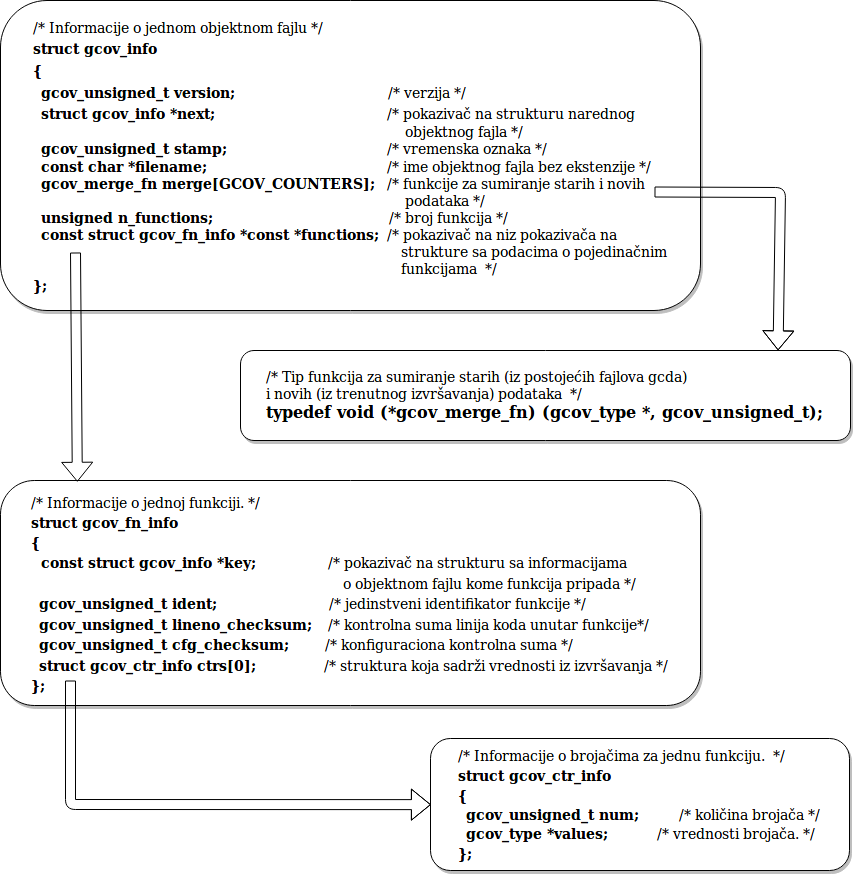
\includegraphics[width=\textwidth]{img/instr_strukture_3.png}
  \caption{Instrumentalizacione strukture i njihove međusobne veze}
  \label{fig:instr}
\end{figure}

Rešenje koje je trenutno implementirano u \strano{GCC}-u, upravo iz tih razloga, sadrži jednog "posrednika" između instrumentalizovanog programa i eksternih alata, a to je \strano{libgcov}. Biblioteka, po svojoj prirodi, se ugrađuje u program i time postaje deo njega, što joj daje ekskluzivno pravo pristupa njegovoj deljenoj memoriji. Njen osnovni zadatak je ekstrakcija podataka iz strukture \kod{gcov\_info} i njihovo konvertovanje u oblik pogodan za obradu eksternim alatom. Statička funkcija \kod{gcov\_at\_exit} preuzima vrednosti brojača, računa sumarne i statističke podatke i sve zajedno upisuje u posebni binarni fajl sa ekstenzijom \strano{gcda} (\strano{GCov DAta file}) u unapred utvrđenom formatu i na unapred utvrđenoj lokaciji. Optimalnost veličine se i ovde postiže primenom sličnih tehnika za kompresiju, kao u slučaju fajla \strano{gcno}. Generiše se uvek pored objetktnog fajla kome odgovara, u slučaju da fajl sa istim imenom i ekstenzijom već ne postoji na toj lokaciji. U slučaju višestrukog pokretanja programa, vrednosti iz predhodnih izvršavanja već se nalaze u fajlu \strano{gcda}, te se on samo ažurira, a za sumiranje starih i novih podataka, zadužena je druga funkcija po imenu \kod{\_\_gcov\_merge\_add\_}. Stoga, za zanemarivanje starih podataka, neophodno je premestiti ili ukloniti prethodni fajl \strano{gcda} pre novog pokretanja.  

Na kraju izvršavanja instrumentalizovanog programa, svi podaci potrebni za informisanje razvojnog tima o pokrivenosti njihovog koda, nalaze se na fajl sistemu i mogu se premeštati i skladištiti. To je veoma korisno, jer pruža nove mogućnosti kombinovanja rezultata različitih merenja. Ukoliko postoji potreba da se neki test prekine na određeno vreme i započne novi, fajlovi \strano{gcda} prvog testa se mogu premestiti na drugu lokaciju, čime će se za drugi test generisati novi, i ponovo prebaciti pored objektnih pred nastavak prvog testa. Za ekonomično skladištenje mogu se koristiti i kompresovane arhive ili eksterni memorijski mediji. Međutim, njihova osnovna funkcija je da predstavljaju ulazne parametre za alat \strano{gcov}, koji na osnovu njih kreira tekstualni izveštaj, pogodniji za interpretaciju od strane razvojnog tima.

Za generisanje jednog izveštaja, potrebno je alatu \strano{gcov} proslediti u vidu argumentata: jedan izvorni fajl, jedan odgovarajući strukturni fajl sa ekstenzijom \strano{gcno} i jedan fajl sa vrednostima brojača sa ekstenzijom \strano{gcda}. Poseban tekstualni fajl sa ekstenzijom \strano{gcov} se kreira za svaki instrumentalizovani fajl izvornog koda. Izveštaj se sastoji od celokupnog sadržaja izvornog koda, uz dodatak jedne vrednosti ispred svake izvršne linije, koja predstavlja broj puta koliko se ta linija izvršavala. Ukoliko se linija nije izvršila nijednom, ispred nje se stavlja posebna oznaka sastavljana od pet simbola tarabice. Prvih nekoliko linija izveštaja rezervisano je za statističke podatke o imenima fajlova od kojih je kreiran, dok se na standardni izlaz štampa najvažnija vrednost: odnos broja izvršenih linija i ukupnog broja linija, odnosno pokrivenost koda. Na listingu \ref{simple}, prikazan je primer osnovnog izveštaja, koji se generiše pozivom alata \strano{gcov} bez dodatnih opcija. Korišćenjem opcija u pozivu alata, izveštaj se može unaprediti i podacima o granama, blokovima i slično. 
\\

\begin{lstlisting}[caption={Primer osnovnog izveštaja koji generiše \strano{gcov}},frame=single, label=simple]
        -:    0:Source:paskal.c
        -:    0:Graph:paskal.gcno
        -:    0:Data:paskal.gcda
        -:    0:Runs:1
        -:    0:Programs:1
        -:    1:#include <stdio.h>
        -:    2:
        1:    3:int main(int argc, char** argv){
        1:    4:    int velicina=atoi(argv[1]),vrednost=1,razmak=0,i,j;
        1:    5:    printf("Paskalov trougao sa %d redova: ",velicina);
        6:    6:    for(i=0; i<velicina; i++){
       20:    7:	for(razmak=1; razmak<=velicina-i; razmak++)
       15:    8:	    printf(" ");
       15:    9:	for(j=0; j<i; j++){
       10:   10:	    if(j==0 || i==0)
        4:   11:		vrednost=1;
        -:   12:	    else
        6:   13:		vrednost=vrednost*(i-j+1)/j;
       10:   14:	    printf("%2d", vrednost);
        -:   15:	}
        5:   16:	printf("\n");
        -:   17:    }
        1:   18:    return 0;
        -:   19:}
\end{lstlisting}

Opcijom -b, izveštaj se obogaćuje statističkim podacima o funkcijama, osnovnim blokovima, granama i pozivima, kao na listingu \ref{branch} Osnovni blok predstavlja jedinicu koda koja se izvršava pravolinijski, odnosno ne sadrži grananja u svojoj unutrašnjosti. Ispred definicije svake funkcije, ispisuje se koliko puta je funkcija pozvana, koliko puta je regularno završena, kao i procenat izvršenih osnovnih blokova u njenoj unutrašnjosti. Nakon završne linije svakog osnovnog bloka, ispisuju se informacije o pokrivenosti poslednjeg grananja ili poziva tog bloka. Za svaku konkretnu granu, prikazuje se procenat odabira te grane u odnosu na ukupan broj prolazaka kroz celo grananje. U slučaju poziva, ta pokrivenost je uglavnom 0 ili 100\%, odnosno izvršeno/neizvršeno. 

\newpage
\begin{lstlisting}[caption={Primer izveštaja koji generiše alat \strano{gcov} sa opcijom -b},frame=single, label=branch]
        -:    0:Source:paskal.c
        -:    0:Graph:paskal.gcno
        -:    0:Data:paskal.gcda
        -:    0:Runs:1
        -:    0:Programs:1
        -:    1:#include <stdio.h>
        -:    2:
function main called 1 returned 100% blocks executed 100%
        1:    3:int main(int argc, char** argv){
        1:    4:    int velicina=atoi(argv[1]),vrednost=1,razmak=0,i,j;
call    0 returned 100%
        1:    5:    printf("Paskalov trougao sa %d redova: ",velicina);
call    0 returned 100%
        6:    6:    for(i=0; i<velicina; i++){
branch  0 taken 83%
branch  1 taken 17% (fallthrough)
       20:    7:	for(razmak=1; razmak<=velicina-i; razmak++)
branch  0 taken 75%
branch  1 taken 25% (fallthrough)
       15:    8:	    printf(" ");
call    0 returned 100%
       15:    9:	for(j=0; j<i; j++){
branch  0 taken 67%
branch  1 taken 33% (fallthrough)
       10:   10:	    if(j==0 || i==0)
branch  0 taken 60% (fallthrough)
branch  1 taken 40%
branch  2 taken 0% (fallthrough)
branch  3 taken 100%
        4:   11:		vrednost=1;
        -:   12:	    else
        6:   13:		vrednost=vrednost*(i-j+1)/j;
       10:   14:	    printf("%2d", vrednost);
call    0 returned 100%
        -:   15:	}
        5:   16:	printf("\n");
call    0 returned 100%
        -:   17:    }
        1:   18:    return 0;
        -:   19:}
\end{lstlisting}

Dodavanjem opcije -a, alatu se sugeriše generisanje podataka o pokrivenosti za svaki osnovni blok ponaosob i njihov ispis ispod poslednje naredbe u okviru tog bloka, kao na listingu \ref{block}. Ukoliko je linija sadržana u više pojedinačnih blokova kao poslednja, sadržaće više podataka o pokrivenosti, tačno jedan za svaki takav blok. 

\newpage
\begin{lstlisting}[caption={Primer izveštaja koji generiše alat \strano{gcov} sa opcijom -a},frame=single, label=block]
        -:    0:Source:paskal.c
        -:    0:Graph:paskal.gcno
        -:    0:Data:paskal.gcda
        -:    0:Runs:1
        -:    0:Programs:1
        -:    1:#include <stdio.h>
        -:    2:
        1:    3:int main(int argc, char** argv){
        1:    3-block  0
        1:    4:    int velicina=atoi(argv[1]),vrednost=1,razmak=0,i,j;
        1:    4-block  0
        1:    5:    printf("Paskalov trougao sa %d redova: ",velicina);
        6:    6:    for(i=0; i<velicina; i++){
        6:    6-block  0
       20:    7:	for(razmak=1; razmak<=velicina-i; razmak++)
        5:    7-block  0
       20:    7-block  1
       15:    8:	    printf(" ");
       15:    8-block  0
       15:    9:	for(j=0; j<i; j++){
        5:    9-block  0
       15:    9-block  1
       10:   10:	    if(j==0 || i==0)
       10:   10-block  0
        6:   10-block  1
        4:   11:		vrednost=1;
        4:   11-block  0
        -:   12:	    else
        6:   13:		vrednost=vrednost*(i-j+1)/j;
        6:   13-block  0
       10:   14:	    printf("%2d", vrednost);
       10:   14-block  0
        -:   15:	}
        5:   16:	printf("\n");
        5:   16-block  0
        -:   17:    }
        1:   18:    return 0;
        1:   18-block  0
        -:   19:}
\end{lstlisting}

\section{Kritika trenutne implementacije u okviru \strano{GCC}-a }


Proučavanjem karakteristika implementacije instrumentalizacije u okviru \strano{GCC}-a i mogućnosti određivanja pokrivenosti koda standardnim \strano{GNU}-ovim alatom: \strano{gcov}-om na osnovu te instrumentalizacije, otkrivena su tri velika nedostatka:

\begin{enumerate}
\item Podaci su dostupni tek po završetku rada programa
\item Korišćenje neoptimalnog statičkog linkovanja
\item Korisnički interfejs standardnog \strano{GNU}-ovog alata ne pruža jednostavan i intuitivan pregled podataka
\end{enumerate}

U narednom tekstu biće detaljnije objašnjeni ovi nedostaci.

\subsection{Prikupljanje podataka na kraju izvršavanja}


Čitanje podataka iz deljene memorije programa i njihovo skladištenje u fajlove \strano{gcda}, odvija se kao poslednja instrukcija programa pre kraja izvršavanja (\kod{at\_exit}). Usled toga, iako analiza \strano{gcov} alatom nije striktno vezana za vremenski tok izvršavanja, ne može se vršiti pre kraja programa. Ovo je veliki nedostatak, koji u nekim specifičnim slučajevima može potpuno onemogućiti proveravanje pokrivenosti koda. Programi kod kojih je vreme rada izuzetno dugo ili su podaci dostupni i/ili korisni samo tokom rada, poput sistema za rad u realnom vremenu, servera ili operativnih sistema, ne mogu koristiti instrumentalizaciju na kraju izvršavanja. Ukoliko imaju ograničene memorijske mogućnosti, što je često slučaj na ovakvim sistemima, ne mogu koristiti ni instrumentalizaciju programskog prevodioca projekta LLVM. Za obezbeđivanje informacija o pokrivenosti koda ovakvih programa, neophodno je proširiti mogućnosti instrumentalizacije \strano{GCC}-a na prikupljanje podataka u toku izvršavanja.


\subsection{Statičko linkovanje}


Biblioteka \strano{libgcov} je u okviru \strano{GCC}-a implementirana kao statička biblioteka (arhiv). Upotreba statičkih biblioteka nije optimalno rešenje \cite{staVSdinLINK}, ni prostorno, ni vremenski. Prilikom linkovanja njeni podaci se kopiraju u program. Ukoliko istu biblioteku koristi više programa, kopiranje će se izvršiti u svaki posebno. Kako se simboli ne razlikuju od programa do programa, ponavljanje je redudantno, što znači da se na ovaj način troši mnogo više memorije nego što je suštinski potrebno. Promene u biblioteci zahtevaju ponovno prevođenje ne samo biblioteke, već i svakog instrumentalizovanog programa ponaosob, što može, zavisno od veličine sistema, predstavljati veliki vremenski utrošak. U sistemu sa neograničenim resursima, prostornim i vremenskim, statički pristup bi predstavljao dovoljno dobro rešenje za instrumentalizaciju bilo kog skupa programa/biblioteka koji taj sistem čini. Međutim, realni sistemi imaju često veoma oštra ograničenja resursa, te je za instrumentalizaciju većeg broja programa/biblioteka potrebno optimizovati sam proces instrumentalizacije, a kao dobra ideja nameće se upotreba dinamičkog linkovanja.


\subsection{Korisnički interfejs}


Prikaz u vidu pojedinačnih izveštaja za svaki fajl izvornog koda, takođe poseduje određene mane. Svaki izveštaj se nalazi na posebnoj lokaciji u okviru direktorijuma projekta, što otežava njihov pregled kao celine. Dodatne informacije, poput onih o pokrivenosti pojedinačnih funkcija, koje se dobijaju dodavanjem opcija u poziv alata, kao i vrednost pokrivenosti fajla, se ne nalaze u okviru izveštaja, već samo ispisa na standardni izlaz, što uzrokuje potencijalni gubitak tih informacija. Vrednost pokrivenosti koda čitavog projekta se ne izračunava, čime je krajnji rezultat oslabljen za još jednu bitnu informaciju. Potreba za prevazilaženjem ovih mana je uticala na formiranje ideje o novom interfejsu za vizuelni prikaz \strano{gcov} statistike, koji je izgrađen u okviru ovog projekta. 


\section{Unapređenje programskog prevodioca \strano{GCC}}


Unapređenje koje je neophodno za korigovanje prethodno navedenih nedostataka može se podeliti u dva odvojena problema:
\begin{enumerate}
\item Unapređenje prikupljanja podataka (poboljšanje \strano{backend} podrške)
\item Unapređenje prikaza podataka (poboljšanje \strano{frontend} podrške)
\end{enumerate}


\subsection{Unapređenje prikupljanja podataka}

Cilj ovog unapređenja jeste omogućiti optimalno prikupljanje podataka iz izvršavanja istrumentalizovanog programa u bilo kom trenutku između početka i kraja programa. U toku projektovanja, bilo je potrebno doneti više važnih odluka koje su značajno odredile tok samog razvoja. Kako je odgovornost za celokupni proces prikupljanja, obrade i prikaza podataka o pokrivenosti koda prevedenog \strano{GCC}-om podeljena između alata \strano{gcov} i biblioteke \strano{libgcov}, prva odluka koju je bilo potrebno doneti jeste odabir materijala za prilagođavanje između ove dve komponente.


\subsubsection{Odabir komponente za prilagođavanje}


Prvobitno je razmatrano rešenje, koje se u ranim fazama projektovanja, linearnom kritičkom razmišljanju nametalo kao očigledno i jednostavno: prilagođavanje alata. Osnovna ideja predstavlja promenu jednog dela ulaznih podataka \strano{gcov}-a, čime bi se vrednosti iz izvršavanja preuzimale direktno iz instrumentalizacionih struktura u deljenoj memoriji programa, umesto iz fajlova \strano{gcda}. Analizom neophodnih izmena za ostvarivanje proširenja mogućnosti na ovaj način, izveden je zaključak da ovo rešenje vodi ka veoma komplikovanoj implementaciji, značajnom padu performansi, kao i ugrožavanju bezbednosti podataka instrumentalizovanog programa. Promena formata ulaznih podataka, iziskivala bi velike algoritamske promene u okviru koda \strano{gcov} programa, čime bi se složenost implementacije gotovo izjednačila sa kreiranjem novog alata. Pristup deljenoj memoriji instrumentalizovanog programa bi predstavljao kritičnu sekciju, usled potencijanog istovremenog upisivanja podataka od strane programa i čitanja istih tih podataka od strane \strano{gcov} alata, zbog čega bi bilo potrebno implementirati određenu vrstu zaštite u vidu zaključavanja ili semafora. Implementacija bi se time dodatno iskompikovala, a performanse, pre svega vremenska složenost, bi značajno opale. Naročito je problematično ugrožavanje performansi instrumentalizovanog programa, jer u cilju pružanja ispravnih informacija, korektna instrumentalizacija mora imati minimalni uticaj na tok i vreme izvršavanja. Bezbednost podataka bi zavisila od kvaliteta implementacije kao i od mogućnosti sistema ukoliko bi bila odabrana naprednija vrsta zaštite. Istrumentalizacione strukture u deljenoj memoriji, po svojoj prirodi su vezane isključivo za trenutno izvršavanje. Stoga bi ovaj pristup takođe ograničio mogućnosti prikupljanja na podatke iz poslednjeg izvršavanja programa. 

Detaljna analiza gore navedenog pristupa, kao i postojeće logike instrumentalizacije implementirane u programskom prevodiocu \strano{GCC}, dovela je do formiranja znatno boljeg rešenja. U trenutnoj implementaciji, celokupni posao prikupljanja podataka prepušten je biblioteci \strano{libgcov}. Promenom trenutka kreiranja fajlova \strano{gcda}, postigao bi se željeni rezultat bez uvođenja dodatnih izazova poput bezbednosti ili algoritamskih promena alata. Detaljnijom analizom ustanovljeno je da je vremenska određenost trenutka izbacivanja rezultata posledica potpune kontrole biblioteke nad instrumentalizacijom, odnosno zatvorenošću interfejsa biblioteke prema potencijalnim korisnicima. Celokupna funkcionalnost je definisana tako da se odvija bez posredovanja vlasnika instrumentalizovanog programa. Ukoliko bi kontola poziva funkcije za generisanje fajlova \strano{gcda} bila prepuštena korisniku biblioteke, prikupljanje podataka bi bilo moguće u bilo kom trenutku. Ovo rešenje je jednostavno za implementaciju, optimalno je, bezbedno i pruža mogućnost kombinovanja rezultata iz više izvršavanja bez dodatnih modifikacija alata za generisanje izveštaja. Četiri navedene prednosti su presudile odabir komponente za prilagođavanje u korist biblioteke \strano{libgcov}. 


\subsubsection{Nova biblioteka, dinamička i nezavisna}


Implementiranje podrške za prikupljanje podataka u toku izvršavanja u vidu biblioteke, otvorilo je mogućnost optimizacije performansi i održavanja "u hodu", ukidanjem zavisnosti od programskog prevodioca i prelaskom na dinamičko linkovanje. Osnovna ideja predstavlja zamenu statičke biblioteke \strano{libgcov} njenim dinamičkim, funkcionalnim pandanom, nezavisnim od infrastrukture \strano{GCC}-a. 

Dinamičko linkovanje znatno poboljšava vremensku složenost u fazi prevođenja, kao i prostornu složenost \cite{staVSdinLINK}. Operativni sistem može smestiti k\^{o}d dinamičke biblioteke u segmente \strano{ROM}-a koje deli više procesa, čime se omogućava jedinstvenost koda u okviru memorije. Time se prostorna složenost sa linerane, svodi na konstantnu vrednost količine memorije potrebne za smeštanje jedne biblioteke, ukidanjem zavisnosti složenosti od broja procesa. Instrukcije biblioteke se ne kopiraju u izvršnu verziju, čime se smanjuje i potreban prostor za skladištenje instrumentalizovanih programa. Dodatne tehnike poput tabela indirekcije i lenjog povezivanja simbola omogućavaju i vremensku uštedu. Sa druge strane, upotreba deljene biblioteke olakšava i procese njene implementacije, testiranja i održavanja. Otklanjanje greške u kodu biblioteke ili potencijana kasnija nadogradnja njenih mogućnosti, ne uslovljavaju ponovno prevođenje svih instrumentalizovanih programa. Prevođenje većih sistema iziskuje dosta vremena, pa ova ušteda pravi značajnu razliku. 

Ukidanje zavisnosi biblioteke za instrumentalizaju od programskog prevodioca omogućava dodatne olakšice kasnijem održavanju, jer nije potrebno ponovno prevoditi celokupni \strano{GCC} nakon svake izmene u kodu biblioteke, a i promena verzije prevodioca ne iziskuje promene u instrumentalizaciji. Ova izmena nema negativan uticaj na performanse, jer se zamenom čuva ukupni skup simbola i instrukcija. 


\subsubsection{Novi interfejs biblioteke}


Korišćenjem nove biblioteke, odgovornost nad pozivom funkcije za ispisivanje podataka u fajlove \strano{gcda} je prebačena na instrumentalizovani program. To je prirodni preduslov pružanja mogućnosti korisniku da sam odabere trenutak u kojem se ta funkcionalnost vrši. 

Osnovni pristup korišćenja podrazumeva definisanje glavne funkcije biblioteke kao eksterne i njen poziv u okviru koda instrumentalizovanog programa. 

Za korisnike \strano{Unix}-a i \strano{Unix}-olikih operativnih sistema, implementirana je jedna dodatna pogodnost. Biblioteka omogućava ispisivanje podataka u fajlove \strano{gcda} pomoću signala \kod{SIGUSR1}. Registracija signala se izvršava u okviru biblioteke na početku izvršavanja. Time se postiže da korisnik nema obavezu da svoj k\^{o}d prilagođava instrumentalizaciji, već može u željenom trenutku, iz terminala poslati signal komandom "kill -10 PID", gde je PID broj koji predstavlja jedinstveni identifikator procesa. Ukoliko korisnik ne može precizno odrediti pravi trenutak na taj način, na raspolaganju mu je i dalje osnovni pristup. Korišćenje signala na \strano{Windows} operativnom sistemu nije podržano, zbog čega je u ovom slučaju neophodno koristiti osnovni pristup. Isti princip važi i ukoliko korisnički program predefiniše signal \kod{SIGUSR1}.


\subsection{Unapređenje prikaza podataka}


Cilj ovog unapređenja jeste omogućiti jednostavan, intuitivan, vizuelni prikaz podataka iz izvršavanja istrumentalizovanog programa. \strano{Gcov} izveštaji i statistički podaci se prikazuju odvojeno od kodova, binarnih i izvršnih fajlova, kako bi se olakšalo i ubrzalo pronalaženje i pregledanje. Prikaz u vidu drveta putanja omogućava brz i efikasan pregled, bez narušavanja modularnosti projekta. Pored osnovnih \strano{gcov} izveštaja, u okviru drveta su dostupni i izveštaji koji sadrže statistiku po funkcijama. 

U okviru novog grafičkog interfejsa za vizuelni prikaz podataka o pokrivenosti koda, pored unapređenja pregleda, implementirano je i nekoliko novih funkcionalnosti. Neki od važnih podataka, poput ukupne pokrivenosti projekta, modula ili programa, ne izračunavaju se pozivom postojećeg alata, zbog njegove ograničenosti na pojedinačni fajl izvornog koda. \strano{Gcov} se može pozvati i sa više argumenta, ali se svaki obrađuje pojedinačno. Interfejs kreiran u okviru ovog projekta, omogućava i prikaz ukupne statistike. Generisanje \strano{gcov} izveštaja za sve izvorne fajlove projekta je dosta olakšano. Umesto višestrukih poziva alata i pozicionaranja u okviru direktorijuma projekta, celokupna funkcionalnost se izvršava jednim klikom. 

Za korisnike \strano{Unix}-a i \strano{Unix}-olikih operativnih sistema, novi grafički interfejs pruža mogućnost i prikupljanja podataka, odnosno slanja signala \kod{SIGUSR1} željenom instrumentalizovanom programu. Time je ukupna funkcionalnost instrumentalizacije dostupna u okviru jedinstvenog grafičkog korisničkog interfejsa. Kao što je već napomenuto, korišćenje signala na \strano{Windows} operativnom sistemu nije podržano, zbog čega je u ovom slučaju za korišćenje novog grafičkog interfejsa preduslov imati već kreirane fajlove \strano{gcda}. Isti princip važi i ukoliko korisnički program predefiniše signal \kod{SIGUSR1}.

% ------------------------------------------------------------------------------
\chapter{Implementacija}
\label{chp:implementacija}
% ------------------------------------------------------------------------------

Implementacija unapređenja prikupljanja i prikaza podataka iz izvršavanja programa prevedenog programskim prevodiocem \strano{GCC} je podeljena u dve zasebne, implementaciono nezavisne celine:
\begin{enumerate}
\item Implementacija dinamičke biblioteke, nezavisne od \strano{GCC}-a, čija osnovna funkcionalnost predstavlja prikupljanje podataka iz izvršavanja programa pre završetka njegovog rada.
\item Implementacija novog grafičkog interfejsa za prikaz podataka, u kome je bezbedna i višegodišnjim korisničkim iskustvom potvrđena osnova, alat \strano{gcov}, nadograđena jednostavnim, preglednim, korisnički prilagođenom interfejsom sa povišenom informativnošću.
\end{enumerate}
U narednom tekstu biće detaljno opisane implementacije obe celine, a celokupan k\^{o}d potreban za njihovu izgradnju je dostupan u okviru \strano{git} repozitorijuma na adresi:\\
\strano{https://github.com/MarinaNikolic/MASTER/tree/master/SRC}


\section{Biblioteka libcoverage}

Implementacija biblioteke \strano{libcoverage} je izvršena u programskom jeziku C. Uzor je predstavljala postojeća bibloteka \strano{libgcov}, podrazumevana biblioteka za prikupljanje podataka iz izvršavanja programa u okviru programskog prevodioca \strano{GCC}. Implementacija je izvšena u četiri faze:
\begin{enumerate}
\item konstrukcija baze biblioteke kao potrebnog i dovoljnog skupa funkcija iz koda prevodioca i biblioteke \strano{libgcov} za prikupljanje podataka,
\item modifikacija vremenskog parametra funkcionalnosti prikupljanja podataka iz izvršavanja, u cilju dostupnosti podataka u toku rada programa,
\item ukidanje zavisnosti biblioteke od prevodioca,
\item vremenska i prostorna optimizacija rešenja.
\end{enumerate}


Osnovna funkcionalnost biblioteke \strano{libgcov} se vrši u okviru funkcije: \kod{gcov\_exit}. Njen algoritam se sastoji iz iterativnih i dubinskih prolazaka kroz instrumentalizacione strukture (prikazane na slici \ref{fig:instr}) u cilju prikupljanja podatka i iz procesa upisivanja tih podataka u binarne fajlove sa ekstenzijom \strano{gcda}. Za prvobitne inicijalizacije, koje je potrebno izvršiti pre poziva funkcije \kod{gcov\_exit}, kao i za upravljanje samim pozivom, zadužena je funkcija \kod{\_\_gcov\_init}. Jedinstveni poziv funkcije \kod{\_\_gcov\_init} na samom početku izvršavanja instrumentalizovanog programa obavlja se nezavisno od koda biblioteke \strano{libgcov}. K\^{o}d poziva se ugrađuje direktno u binarni k\^{o}d programa u toku prevođenja, uz uslov prisustva flegova za instrumentalizaciju. Stoga je k\^{o}d ove dve funkcije najpre izdvojen da, uz određene modifikacije, predstavlja bazu nove biblioteke. 

Važno je napomenuti da se k\^{o}d biblioteke \strano{libgcov} razlikuje u zavisnosti od verzije prevodioca \strano{GCC}. U prethodnom poglavlju, predstavljena je šira slika, pre svega funkcionalnosti, bez implementacionih detalja. Stoga, u tom trenutku, nije bilo potrebno ograničavati se na konkretnu verziju. Princip koji se trenutno opisuje je karatkeristika isključivo verzija starijih od 5.1.0. Implementacija biblioteke \strano{libcoverage} je rađena po uzoru na k\^{o}d prevodioca verzije: 4.8.0. Pojedine specifične funkcionalnosti su preuzimane iz ranijih ili kasnijih verzija, u cilju optimizacije ili osamostaljivanja. 

Ostatak koda koji je preuzet iz \strano{GCC}-a, bilo u celosti, parcijalno ili uz modifikacije, dodat je isključivo u cilju definisanja nerazrešenih simbola prilikom osamostaljivanja biblioteke od prevodioca. Dakle, tokom prve faze implementacije je, na osnovu iscrpne analize strukture i funkcionalnosti onih modula prevodioca \strano{GCC}, koji omogućavaju prikupljanje podataka iz izvršavanja programa, kreirana samoodrživa, ali još uvek ne funkcionalna baza nove biblioteke. 

Druga faza implementacije obuhvatala je potrebne modifikacije u cilju postizanja prikupljanja podataka iz izvršavanja programa u toku njegovog rada. Rad alata \strano{gcov}, koji rezultuje finalnim izveštajima, nije zavistan od izvršavanja programa, već samo od dostupnosti ulaznih argumenata: izvornog koda i fajlova \strano{gcno} i \strano{gcda}. Kako su fajlovi \strano{gcno} dostupni već nakon prevođenja izvornog koda do objektnih fajlova, za ostvarenje željene funkcionalnosti je potrebno i dovoljno modifikovati trenutak nastajanja fajlova \strano{gcda}. Uslovljenost završetkom rada programa, je suštinski uzrokovana time što se u okviru funkcije \kod{\_\_gcov\_init}, za čije je bezuslovno izvršavanje dovoljno prevesti k\^{o}d sa instrumentalizacionim flegovima, poziva funkcija \kod{gcov\_exit} kao argument \kod{atexit} funkcije standardne biblioteke \strano{stdlib}. Eliminacijom ovog poziva, postignut je prvi korak ka prikupljanju podataka u proizvoljnom trenutku rada programa. Nakon ovog koraka, naziv \kod{gcov\_exit} je postao neprikladan i konfuzan, pa je izvršena njegova korekcija. U novoj biblioteci \strano{libcoverage}, funkcija \kod{gcov\_exit} je preimenovana u \kod{drew\_coverage} \footnote{Na odabir naziva uticale su isključivo estetske i lične preferencije autora.}. Drugi korak predstavlja pružanje mogućnosti korisniku da sam odabere trenutak u kome će se poziv funkcije izvršiti. Zaglavlje \strano{coverage.h}, koje takođe ulazi u izgradnju nove biblioteke, sadrži deklaraciju funkcije: \kod{drew\_coverage}. Stoga je dovoljno da se u korisnčkom kodu, na željenoj lokaciji, uključi ovo zaglavlje ili funkcija navede kao eksterna, a zatim regularno pozove. Razrešavanje simbola nastalih ovim pozivom, biće obavljeno u fazi linkovanja biblioteke \strano{libcoverage.so}.

Za korisnike \strano{Unix}-a i \strano{Unix}-olikih operativnih sistema, implementirana je i mogućnost poziva korišćenjem signala \strano{SIGUSR1}. Za ostvarivanje ove pogodnosti, neophodno je navesti u fazi linkovanja dodatni objektni fajl: \strano{coverage\_registration.o}. K\^{o}d, čijim prevođenjem nastaje ovaj objektni fajl, prikazan je u okviru listinga \ref{registrator}. Pisan je u programskom jeziku C i u celosti se nalazi u okviru fajla:  \strano{coverage\_registration.c}. Sastoji se iz dve funckije: \kod{coverage\_signal\_registry} i \kod{coverage\_handler}. Prva funkcija predstavlja alternativni \strano{signal-handler} za \strano{SIGUSR1}, u okviru koga se izvršava poziv funkcije: \kod{drew\_coverage}. Druga funkcija je zadužena za registrovanje funkcije \kod{coverage\_handler} kao \strano{signal-handler} za \strano{SIGUSR1}, a korišćenjem \kod{\_\_attribute\_\_((constructor))} principa, vezana je za sam početak izvršavanja instrumentalizovanog programa \footnote{Navođenjem jednog od specijalnih atributa: konstruktor funkcija (\kod{\_\_attribute\_\_((constructor))}) / destruktor funkcija (\kod{\_\_attribute\_\_((destructor))}), u okviru deklaracije funkcije, uslovljava se njeno pozivanje pre/nakon funkcije \kod{main()}. To se postiže tako što se funkcije, označene na ovaj način, smeštaju tokom prevođenja u posebnu sekciju objektnog fajla, po imenu \kod{.ctors} / \kod{.dtors}.}. 

Korišćenje ove metode je opciono i zavisi isključivo od želje korisnika i mogućnosti korišćenja signala datog programa. Ukoliko operativni sistem ne podržava \strano{POSIX} signale ili korisnički k\^{o}d predefiniše signal \strano{SIGUSR1}, ovaj princip se ne može koristiti.

\newpage

\begin{lstlisting}[caption={Izvorni k\^{o}d u okviru fajla: \strano{coverage\_registration.c}},frame=single, label=registrator]
#include <stdio.h>                                                       
#include <signal.h>                                                      
#include <unistd.h>     

#define COVERAGE_SIGNAL SIGUSR1
extern void drew_coverage();

void coverage_handler(int signo){
    if (signo==COVERAGE_SIGNAL){
         printf("Dumping coverage data... \n");
    drew_coverage();
    }
}

__attribute__((constructor))
void coverage_signal_registry(){
    printf("Registrating signal SIGUSR1 for coverage data dump...\n");
    signal(SIGUSR1,coverage_handler);
}
\end{lstlisting}

Pored osnovnih izmena, izvršene su i dve manje modifikacije funkcije za prikupljanje podataka i kreiranje fajlova \strano{gcda}. Konstanta \kod{GCOV\_LOCKED}, definisana pretprocesorskom direktivom, a korišćena u cilju sprečavanja paralelizacije rada funkcije \strano{gcov\_exit} iz biblioteke \strano{libgcov} i alata \strano{gcov}, izbačena je iz upotrebe. U novom pristupu, paralelizacija procesa prikupljanja i obrade podataka je, iako bezbednosni izazov, poželjna osobina. Međutim, celokupni k\^{o}d koji koristi globalnu promenljivu \kod{gcov\_dump\_complete}, zadužen za sprečavanje višestrukog izbacivanja podataka o izvršavanju programa, kao i sama promenljiva nisu eliminisani. Bez alternativnog mehanizma odbrane, eliminacija ove funkcionalnosti bi dovela do netačnih vrednosti u izveštaju, odnosno vrednosti multipliciranih brojem poziva funkcije za ispis. Prebacivanje odgovornosti premeštanja starih fajlova \strano{gcda} pre novog poziva funkcije, nije prihvatljivo rešenje sa stanovišta bezbednosti i jednostavnosti upotrebe, dok bi automatsko naknadno prepakivanje fajlova \strano{gcda} narušilo kompatibilnost sa postojećim interfejsom trenutne implementacije. 

Cilj treće faze implementacije predstavlja uklanjanje zavisnosti biblioteke od programskog prevodioca \strano{GCC}. Prvi korak ka tom cilju, obavljen je još u toku prve faze, dodavanjem određenih funkcija i konstanti iz koda prevodioca, neophodnih za definisanje simbola, koji su u fazi linkovanja označeni kao nerazrešeni. U cilju logičkog osamostaljivanja i sprečavanja višestruke definisanosti simbola, funkcije koje programski prevodilac \strano{GCC} koristi i van procesa instrumentalizacije, su zamenjene sličnim, funkcionalno kompatibilnim, varijantama. Primer je funkcija: \kod{gcc\_assert}, koja je zamenjena varijantom preuzetom iz verzije 5.0, pod nazivom: \kod{gcov\_nonruntime\_assert}. Ukinuta je zavisnost od definisanosti promenljive \kod{IN\_LIBGCOV}, koja uslovljava prikupljanje podataka postojećom bibliotekom \strano{libgcov}, na kraju izvršavanja programa. 

Ukidanje zavisnosti biblioteke od prevodioca, odnosno omogućavanje njenog samostalnog prevođenja, prouzrokovalo je da biblioteka izgubi informaciju o verziji prevodioca. Različitost implementacije instrmentalizacije i prikupljanja podataka kroz verzije prevodioca \strano{GCC}, morala se prevazići ograničavanjem na konkretnu verziju ili dodatnim modifikacijama. Kako prva opcija suštinski poništava efekat nezavisnosti biblioteke, doneta je odluka da se, u okviru četvrte faze implementacije, izvrše dodatna prilagođavanja koda biblioteke u cilju postizanja što veće multiverzionalnosti. U okviru izmena koje su objavljene pod verzijom 4.7.0. izvršen je i veći redizajn, ne samo procesa prikupljanja podataka, već i samog formata instrumentalizacionih struktura. Prilagođavanje biblioteke radu sa strukturama definisanim na stari način, iziskivalo bi izgradnju potpuno nove biblioteke, što predstavlja nepotreban napor. Takođe, aktuelna verzija \strano{GCC}-a u vreme ove implementacije je bila 6.2. što predstavlja gornje ograničenje multiverzionalnosti biblioteke \strano{libcoverage.so}. Kasnijom analizom utvrđena je kompatibilnost i sa ostalim podizdanjima u okviru izdanja 6. U cilju izgradnje jedinstvene biblioteke za sve verzije \strano{GCC}-a, počevši od 4.7.0. i zaključno sa 6.5.0., najpre su iz koda eliminisane sve provere verzije prevodioca, alata \strano{gcov} i fajlova \strano{gcno} i \strano{gcda}. 

Uveden je novi mehanizam određivanja verzije koji osigurava isključivo poklapanje verzije u fajlovima \strano{gcno} i \strano{gcda}, neophodno za rad alata \strano{gcov}. 
Globane vrednosti unutar same biblioteke koje su zavisne od verzije prevodioca, prilagođavaju se verziji pretprocesorskim direktivama. Prilagođavanje količine brojača koji se koriste za instrumentalizaciju, definisane promenljivom \kod{GCOV\_COUNTERS} prikazano je u okviru listinga \ref{brojaci}.

\newpage

\begin{lstlisting}[caption={Definisanje količine brojača u zavisnosti od verzije prevodioca},frame=single, label=brojaci]
#if __GNUC__ == 6
#define GCOV_COUNTERS 10
#elif __GNUC__ == 5 && __GNUC_MINOR__ >= 1
#define GCOV_COUNTERS 10
#elif __GNUC__ == 4 && __GNUC_MINOR__ >= 9
#define GCOV_COUNTERS 9
#else
#define GCOV_COUNTERS   8
#endif
\end{lstlisting}

Poslednja faza implementacije obuhvata izmene vršene u cilju vremenske i prostorne optimizacije. U starijim verzijama prevodioca \strano{GCC}, računanje glavne kontrolne sume programa se obavljalo na početku izvršavanja, u okviru funkcije \kod{\_\_gcov\_init}. Korišćen je mehanizam pod nazivom: ciklična provera pariteta bloka, nad statičkim podacima programa (imena instrumentalizovanih fajlova izvornog koda). Od verzije 4.7.0, uveden je novi algoritam, po kome se ova kontrolna suma računa u toku čitanja podataka iz instrumentalizacionih struktura, u okviru funkcije \kod{gcov\_exit}. Mehanizam ciklične provere pariteta bloka je zadržan, ali je skup podataka potpuno izmenjen. Umesto imena fajlova, koriste se drugi statički podaci, kao što je broj funkcija, a uključeni su i dinamički podaci, odnosno vrednosti brojača. Eventualna oštećenja podataka će sa dovoljno velikom verovatnoćom biti detektovana u kontrolnim sumama pojedinačnih entiteta, pre svega funkcija, pa dinamičko računanje kontrolne sume programa troši više vremena nego što doprinosi. Stoga su, u novoj biblioteci, kontrolne sume implementirane po uzoru na verziju 4.6.0. 

Dodatna optimizacija postignuta je redukovanjem broja sistemskih poziva za ispisivanje sadržaja u fajl \strano{gcda}. Umesto velikog broja manjih poziva sistemskog poziva \strano{write} za svaku 32-obitnu vrednost oznake ili brojača, vrši se jedinstveni poziv za celokupan sadržaj jednog fajla \strano{gcda}. Kako se bafer za privremeno čuvanje ne reciklira, već samo proširuje, ovim se nije povećala prostorna složenost. Dodatni memorijski prostor je potreban samo za skladištenje jedne dodatne globalne promenljive koja sadrži broj trenutno neispisanih vrednosti. Sa druge strane, procesoru je prepuštena odluka o veličini pojedinačnog bloka koji će se upisati, što je na sistemu optimalna vrednost. 

Računanje vrednosti histograma je takođe izbačeno iz trenutne implementacije biblioteke \strano{libcoverage}, pošto se vrednosti nisu koristile ni u jednom dokumentovanom slučaju upotrebe. Prisustvo histograma je zadržano isključivo u definiciji odgovarajuće instrumentalizacione strukture, u cilju kompatibilnosti sa prevodiocem. 

Manja ušteda prostora je ostvarena i uvođenjem pravolinijskog prolaska kroz strukture. Umesto alociranja privremenog pokazivača na međustrukturu, kao što je prikazano u gorenjem delu slike \ref{pristup}, korišćen je pravolinijski pristup prikazan u donjem delu iste slike. 

\begin{lstlisting}[caption={Pristup instrumentalitacionim strukturama},frame=single, label=pristup]
definicija: gfi_ptr = gi_ptr->functions[f_ix];
definicija: ci_ptr = gfi_ptr->ctrs;
pristup:    ci_ptr->values;
==>	
pristup:    gi_ptr->functions[f_ix]->ci_ptr->values
\end{lstlisting}

\section{Korisnički interfejs}

Implementacija novog grafičkog interfejsa za prikaz podataka iz izvršavanja programa, pod nazivom: \strano{code\_coverage\_viewer}, izvršena je u programskom jeziku \strano{Python}, korišćenjem posebnog modula za grafičku podršku: \strano{wxPython}. Osnovna uloga novog interfejsa jeste da predstavlja jednostavni, pregledni, korisniku prilagođen omotač za celokupan proces prikupljanja i prikaza podataka u toku izvršavanja programa. Usled pružanja dodatnih informacija o statistici pojedinačnih modula i/ili celokupnog projekta, \strano{code\_coverage\_viewer} je i više od interfejsa.

Grafički korisnički interfejs se sastoji iz dve celine: kontrolne i prezentacione, i jedne linije menija. Celine su implemenatciono predstavljene sa dva \strano{skroll}-ujuća panela (\kod{wx.Panel}), dobijena pomoću vertikalnog splitera ekrana (\kod{wx.SplitterWindow}), dok je za kreiranje menija korišćena klasa \kod{wx.MenuBar}. Na slici \ref{fig:GUI1} je dat prikaz grafičkog korisničkog interfejsa nakon pokretanja. Osnovne komponente, čije će osobine i funkconalnosti biti objašnjenjene u  nastavku, vidljive su i dostupne odmah po pokretanju. 

\begin{figure}[!ht]
  \centering
  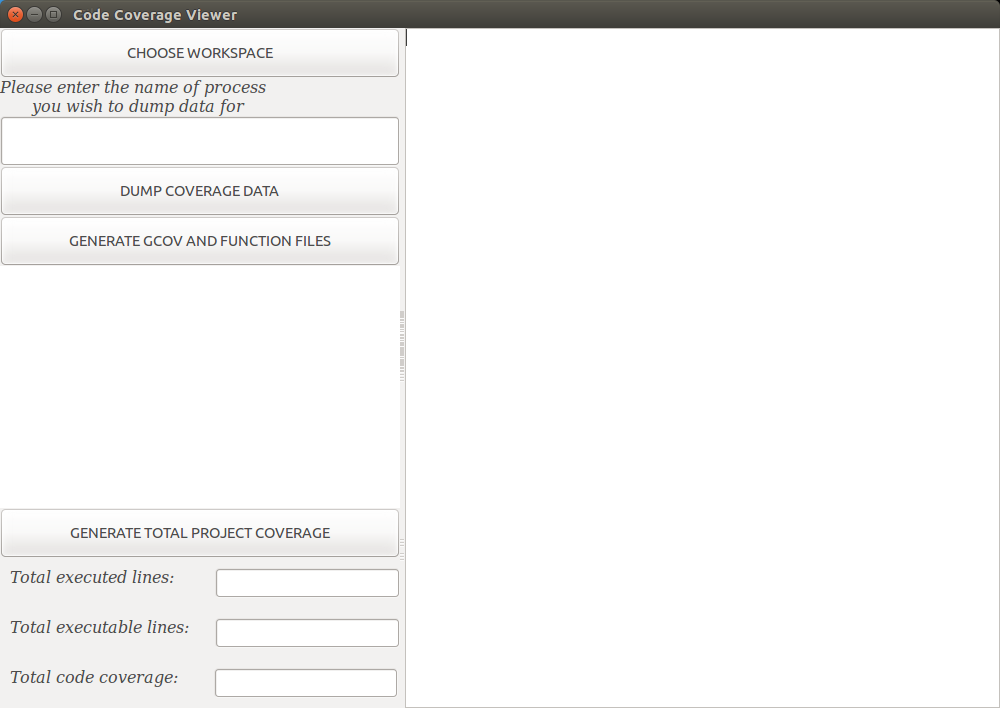
\includegraphics[width=\textwidth]{img/GUI_1_ng.png}
  \caption{Grafički interfejs po pokretanju}
  \label{fig:GUI1}
\end{figure}


Kontrolna celina se proteže levom stranom interfejsa, zauzimajući okvirno jednu trećinu ukupnog prostora. Sadrži deset komponenti, raspoređenih u jedinstvenu kolonu. 

Na samom vrhu se nalazi dugme za odabir radnog direktorijuma: \strano{Choose workspace}, kreirano korišćenjem klase \kod{wx.Button}. Klikom na ovo dugme, otvara se novi prozor, instanca klase \kod{wx.DirDialog}, kao na slici \ref{fig:GUI2} Pomoću njega se, navigacijom kroz sistem datoteka, odabira koreni direktorijum projekta ili pojedinačne komponente, za koju korisnik želi podatke o pokrivenosti. Nakon odabira, prozor za dijalog se zatvara i vrši se ažuriranje drvolike strukture koja oponaša strukturu odabranog direktorijuma. Više detalja o njoj, biće u nastavku teksta. Ukoliko se u njemu direktno ili rekurzivno nalaze već generisani izveštaji, oni će biti adekvatno prikazani u drvolikoj strukturi i za njih će važiti celokupna dalja funkcionalnost interfejsa. 

Sledeće tri komponente u koloni čine tekstualno polje za unos imena procesa, labela za pružanje informacije šta u to polje treba uneti i dugme za kreiranje fajlova \strano{gcda}. Tekstualno polje je instanca klase za prikaz dinamičkog teksta, pod nazvom: \kod{wx.TextCtrl}, i služi za unos imena procesa kome treba poslati signal da prikupi podatke o svom dotadašnjem izvršavanju i upiše ih u fajlove sa ekstenzijom \strano{gcda}. Ukoliko se na sistemu izvršava više programa sa tim imenom, signal će biti poslat svakom posebno. Sama funkcionalnost korišćenja komande \strano{kill} za slanje signala \strano{SIGUSR1} u cilju prikupljanja podataka, odnosno pozivanja funkcije \kod{drew\_coverage} iz biblioteke \strano{libgcov}, se ne pokreće već nakon upisa imena, već je potreban klik na dugme za kreiranje fajlova \strano{gcda}, pod nazivom \strano{Dump coverage data}. Ovo dugme je takođe instanca klase \kod{wx.Button}, kao i prethodno, dok je za sve labele korišćena klasa za prikaz statičkog teksta, pod nazivom: \kod{wx.StaticText}. 


Funkcionalnost ove tri komponente je dostupna samo korisnicima \strano{Unix} ili \strano{Unix}-olikih sistema, koji su pored instrumentalizacionih flegova i biblioteke \strano{libcoverage}, svoj program preveli i koristeći objektni fajl \strano{coverage\_registration.o}, i nisu predefinisali signal \strano{SIGUSR1}. Ograničenje je napomenuto u specifikaciji grafičkog korisničkog interfejsa, kao i u okviru \strano{Help}-a. 

Izvršavanje sistemske komanade \kod{kill -10 <pid>}, kao i svih ostalih sistemskih komandi je implementirano pomoću funkcije \kod{system}, modula \kod{os}. Ovo je najjednostavniji princip, bez bezbednosnih izazova, koji u potpunosti zadovoljava potrebe novog grafičkog interfejsa. Naredne dve komponente predstavljaju interfejs ka funkcionalnosti generisanja izveštaja alatom \strano{gcov} i kontrole njihovih prikazivanja. Dugme: \strano{Generate gcov and function files} pokreće rekurzivnu pretragu radnog direktorijuma i poziv alata \strano{gcov} za sve pronađene fajlove \strano{gcda}. Odgovarajući fajl \strano{gcno} se nalazi na istoj lokaciji gde i \strano{gcda}, dok se putanja do fajla sa izvornim kodom dobija parsiranjem sadržaja fajla \strano{gcno}. Ovim postupkom se kreiraju dva tipa izveštaja: 
\begin{enumerate}
\item Standardni izveštaji sa ekstenzijom \strano{gcov}, koji sadrže kvantitativne podatke za svaku izvršnu liniju koda
\item Funkcijski izveštaji sa ekstenzijom \strano{fun}, koji sadrže podatke o pokrivenosti pojedinačnih funkcija i ukupnu pokrivenost fajla izvornog koda
\end{enumerate}
Kreiranje oba tipa izveštaja se vrši jedinstvenim pozivom alata, sa jednom dodatnom opcijom: \kod{-f}. Alat \strano{gcov} sam generiše standardni izveštaj, dok sadržaj funkcijskog izveštaja predstavlja preusmereni ispis na standardni izlaz. 

Svi izveštaji se smeštaju u drvoliku strukturu, lociranu ispod dugmeta za njihovo generisanje, koja je implementirana kao instanca klase \kod{wx.TreeCtrl}. Celokupni sadržaj se briše, a drvolika struktura se ponovo izgrađuje, popunjavajući se novim podacima. Ista procedura se vrši, kao što je već napomenuto, i prilikom promene radnog direktorijuma. Ova struktura ima dvostruku ulogu. Pored intuitivnog prikaza imena i lokacije svakog izveštaja, u vidu drveta koje oponaša strukturu radnog direktorijuma, služi i kao kontrolna jedinica za prikaz sadržaja u desnoj celini grafičkog korisničnog interfejsa. Prikaz sadržaja željenog izveštaja se pokreće jednim klikom na njegovo ime. 

Na samom dnu leve celine nalazi se skup od četiri komponente koje služe za određivanje i prikaz ukupne pokrivenosti koda u okviru radnog direktorijuma: jedno dugme i tri kompozitne strukture. Dugme \strano{Generate total project coverage} pokreće računanje tri podatka: ukupan broj izvršnih linija, ukupan broj izvršenih linija do trenutka kreiranja fajlova \strano{gcda} i procenat koji označava ukupnu pokrivenost koda u okviru odabranog radnog direktorijuma. Svaka od tri kompozitne strukture sadrži po jedno tekstualno polje za prikaz jednog od tako izračunatih podataka i labelu za objašnjenje sadržaja tekstualnog polja. Sam proces računanja zahteva parsiranje standardnih izveštaja u cilju ekstrakcije kvantitativnih podataka izvršenosti pojedinačnih linija i može biti veoma vremenski zahtevan. Stoga nije izvršavan u okviru procesa generisanja izveštaja, već kao zasebna funkcionalnost. Ukupna vremenska složenost je veća pri ovakvom pristupu, ali je vreme potrebno za dobijanje prvih podataka prilično redukovano. U toku izračunavanja ukupne pokrivenosti, korisniku su na raspolaganju pojedinačni izveštaji za pregledanje i analizu. Prikaz grafičkog korisničkog interfejsa nakon generisanja izveštaja i računanja ukupne pokrivenosti dat je na slici \ref{fig:GUI3}.

\begin{figure}[!ht]
  \centering
  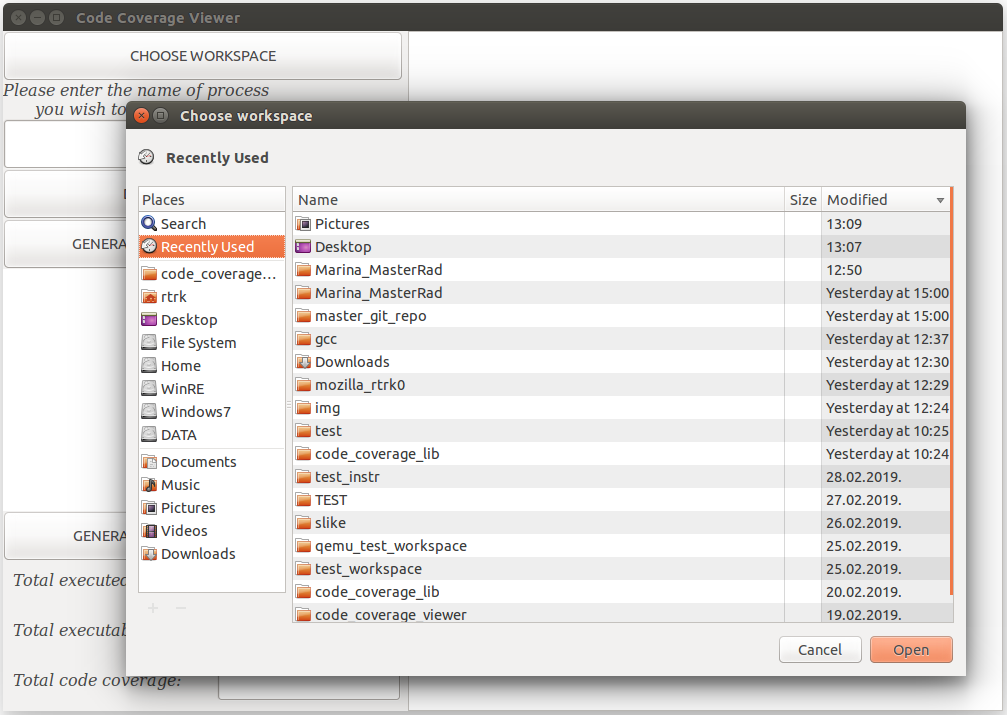
\includegraphics[width=\textwidth]{img/GUI_2_ng.png}
  \caption{Odabir radnog direktorijuma u grafičkom interfejsu}
  \label{fig:GUI2}
\end{figure}

\begin{figure}[!ht]
  \centering
  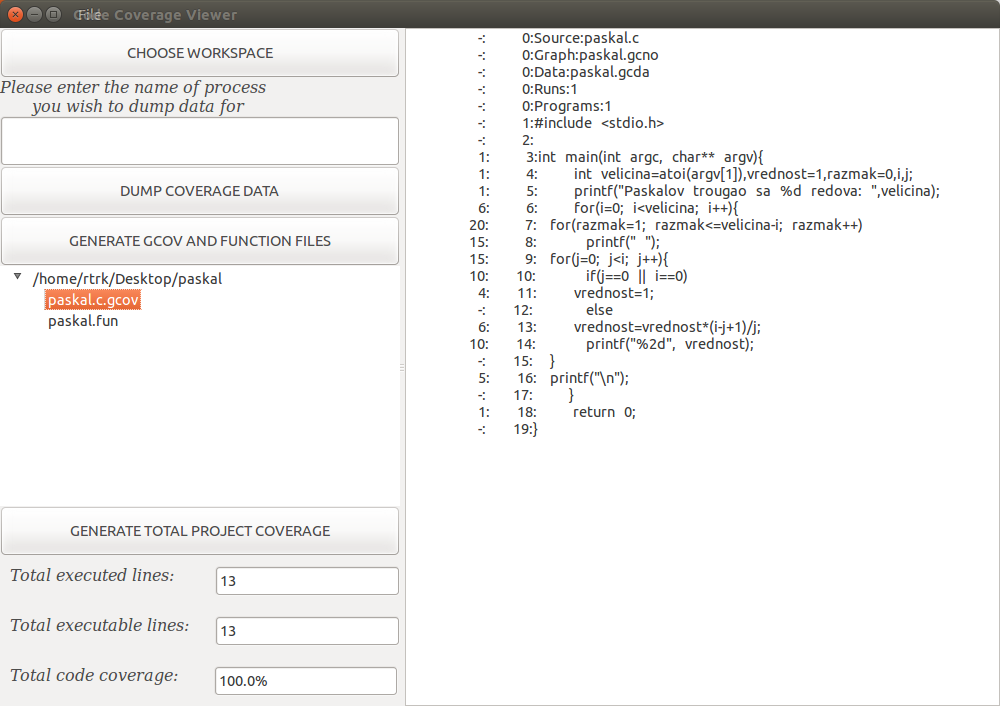
\includegraphics[width=\textwidth]{img/GUI_3_ng.png}
  \caption{Generisana celokupna statistika prikazana u grafičkom interfejsu}
  \label{fig:GUI3}
\end{figure}

Prezentaciona celina se proteže desnom stranom interfejsa, zauzimajući okvirno dve trećine ukupnog prostora. Sadrži svega jednu komponentu, koja služi za prikaz sadržaja konkreknog izveštaja, odabranog pomoću drvolike strukture leve celine. Implementirana je kao instanca klase za prikaz dinamičkog teksta: \kod{wx.TextCtrl}, čime se pruža dodatna mogućnost kopiranja sadržaja, menjanja ili brisanja. Prikaz izveštaja koji sadrže ne-\strano{ASCI} karaktere, omogućen je korišćenjem unapređene azbuke koju nudi paket: \kod{ISO-8859-1}. Postavljen je kao podrazumevani paket, kako bi se unapredila i upotrebna vrednost funkcionalnosti odabira radnog direktorijuma, ali i omogućilo čitanje fajlova \strano{gcno}. 

Linija menija je implementirana korišćenjem klase \kod{wx.MenuBar}. Sadrži ime novog interfejsa i jedno dugme, tipa \kod{wx.Menu}, pod nazivom \strano{File}. Jednim klikom na dugme \strano{File}, pojavljuje se lista sa dve opcije: \strano{Help} i \strano{Quit}. Odabiranjem opcije za pomoć, na centru ekrana se pojavljuje novi prozor, klase \kod{wx.PopupWindow}, kao na slici \ref{fig:GUI4}. Prozor se sastoji iz jedinsvenog panela, čiju celokupnu površinu zauzima tekstualno polje, statičke prirode, sa kratkim uputstvom za upotrebu grafičkog interfejsa. Prozor je mobilan, što je ostvareno pomoću preračunavanja kordinata, a nakon korišćenja, može se zatvoriti desnim klikom na bilo koju tačku njegove površine. Opcija \strano{Quit} služi za zatvaranje glavnog prozora interfejsa.

\begin{figure}[!ht]
  \centering
  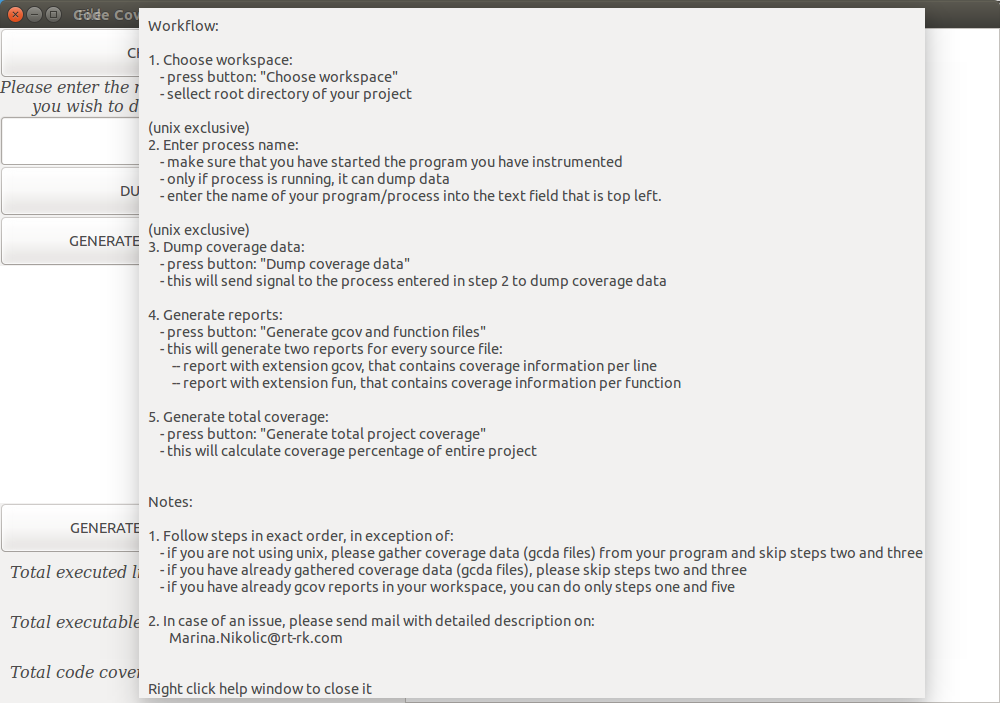
\includegraphics[width=\textwidth]{img/GUI_4_ng.png}
  \caption{Prozor za pomoć u grafičkom interfejsu}
  \label{fig:GUI4}
\end{figure}
 
U okviru specifikacije novog grafičkog interfejsa, kao i u okviru \strano{Help}-a, detaljno je opisana pravilna upotreba. 

Za korisnike koji nemaju naviku da čitaju dokumentacije, specifikacije i pomoćne sadržaje, osmišljen je mehanizam podsvesnog navođenja. Naime, redosled komponenti kontrolne celine je osmišljen i implementiran na način koji ima za cilj podsvesno navođenje korisnika na pravilni redosled upotrebe. Akcije donjih skupova komponenti su u velikoj meri uslovljene akcijama onih iznad, što uslovljava korišćenje "odozgo na gore". Poslednji stepen zaštite od nepravilne upotrebe nalazi se na nivou pojedinačne komponente i onemogućava njen rad, ukoliko potrebni uslovi nisu ispunjeni. Ispunjenost uslova se određuje stanjem radnog direktorijuma i programa, a ne izvršenosti funkcionalnosti grafičkog interfejsa, čime su pokriveni i slučajevi parcijalne upotrebe, kao na primer, pregledanje već generisanih izveštaja. Takođe, tom prilikom se korisniku otvara i mali prozor za dijalog, instanca klase \kod{wx.MessageDialog}, pomoću koga se informiše o konkretnoj grešci u proceduri i dobija savet o adekvatnom sledećem koraku.


% ------------------------------------------------------------------------------
\chapter{Analiza korektnosti i performasi}
\label{chp:testiranje}
% ------------------------------------------------------------------------------

\section{Analiza performansi}

U okviru analize performansi softverskog rešenja za prikupljanje i prikaz podataka o pokrivenosti koda u toku izvršavanja, ispitivanje je sprovedeno prema tri kriterijuma:
\begin{enumerate}
\item Bezbednost
\item Složenost
\item Jednostavnost upotrebe
\end{enumerate}

\subsection{Bezbednost}

Bezbednost predstavlja jednu od najvažnijih karakteristika softvera kao proizvoda, naročito kada je reč o višenamenskim rešenjima, kao što je slučaj sa bibliotekom \strano{libgcov}. Od nivoa ispunjenosti ovog kriterijuma, direktno zavisi i djapazon potencijalne upotrebe softverskog rešenja. U okruženja koja predstavljaju naročiti bezbednosni izazov svrstavamo najpre one sisteme od čije ispravne funkcionalnosti zavise ljudski životi, ekonomski značajni resursi i poverljivost važnih informacija. Teorijsko ispitivanje bezbednosti rešenja opisanog u ovom radu je izvršeno analizom upravljanja memorijskim resursima i mogućnosti neovlašćenog pristupa. 

Analizom izvornog koda biblioteke \strano{libcoverage}, utvrđeno je da se ukupna dinamički alocirana memorija, oslobođa naredbama: \kod{free(gcov\_var.buffer)} i \\ \kod{fclose(gcov\_var.file)} \\
Za dokazivanje ove tvrdnje, odnosno detektovanje eventualnog nepravilnog upravljanja memorijom, iskorišćen je standardni alat za memorijsko profajliranje: \strano{Valgrind}. Ovaj alat nema mogućnost ispitivanja biblioteke, kao neizvršne jedinice sistema, zbog čega je bilo neophodno analizu sprovesti nad eksternim izvršnim programom. Korektnost rezultata je postignuta uključivanjem biblioteke u sistem, čija je bezbednost unapred potvrđenjena istim alatom. Porukom: \strano{ERROR SUMMARY: 0 errors from 0 contexts (suppressed: 0 from 0)}, dokazano je da biblioteka ne prouzrokuje curenje memorije, pisanje van alociranog prostora, niti slične propuste. 

Neovlašćeni pristup podacima programa je sprečen prirodom rešenja za prikupljanje i prikaz podataka. Implementacija softverskog rešenja za prikupljanje u vidu biblioteke, nasuprot eksternog alata, čini program jedinim vlasnikom podataka sopstvene deljene memorije. Rešenje koje za formatiranje i prikaz, koji za transport i obradu podataka ne koristi internet, niti bilo koju drugu mrežu, je dodatno otpornim na napade eksterne prirode. Time je ispunjen bezbednosni aspekt zaštite podataka od neovlašćenog pristupa. 

\subsection{Složenost}

Algoritam prikupljanja podataka iz deljene memorije programa nije promenjen u odnosu na postojeću implementaciju. Optimizacija ispisa u fajlove \strano{gcda} je zavisna od ulaznih podataka i okruženja instrumentalizovanog programa i ne menja kvantitet jedinica za obradu, te ne utiče na procenu algoritamske složenosti. Ekvivalencija vremenske i prostorne zavtevnosti procesa prikupljanja podataka o pokrivenosti koda sa postojećom bibliotekom \strano{libgcov} se može postići pozivom funkcije \kod{drew\_coverage} kao argumenta \kod{atexit} funkcije. Zbog toga, složenost kao karatkeristika najzahtevnojeg slučaja, ostaje nepromenjena. Unapređenje performansi se može primetiti tek prilikom posmatranja prosečnog slučaja. Ranijim pozivom funkcije za prikupljanje podataka, smanjuje se količina ulaznih podataka algoritama, što u velikim sistemima, sa velikom količinom koda može dovesti do značajnog smanjenja potrebnih vremenskih i prostornih resursa. 

Do značajna uštede može se doći i prilikom instrumentalizacije kodova sa visokim procentom dugih, repetativnih jedinica u slučaju da postoji interesovanje samo za procenat pokrivenosti koda. Izvršavanje pojedinačne linije više od jednog puta, nema uticaj na računanje pokrivenosti koda, već samo na pojedinačne izveštaje. Za postizanje stoprocentne pokrivenosti, teorijski je dovoljno izvršiti svaku liniju samo jednom. Stoga prekidanje prikupljanja podataka pre kraja izvršavanja može u ovakvim slučajevima dati korektne rezultate uz upotrebu znatno manje količine resursa. Kao posledica, nastaje novi oblik testiranja programa, koji možemo nazvati: testiranje vođeno pokrivenošću. Detaljan opis biće dat kroz ilustrativan primer. Program koji će biti posmatran predstavlja server za pružanje informacija iz neke baze podataka. U zavisnosti od klijenta, server izvršava različite \strano{SQL} upite nad bazom, obrađuje rezultat i informiše klijenta. Pokretanjem servera izvršava se inicijalni deo koda, nakon čega serverska aplikacija prelazi u stanje čekanja. Ukupan broj izvršnih linija koda servera možemo označiti sa \kod{N}, a broj izvršnih linija u segmentu koda za prekid rada servera sa \kod{M}. Kod zadužen za pokretanje aplikacije i obradu svih različitih zahteva stoga ima N-M izvršnih linja, te ćemo oceniti targetiranu pokrivenost na \kod{(N-M)/100} procenata. Cilj testiranja predstavlja pokrivanje svih slučajeva upotrebe i analiza ponašanja aplikacije. Ideja testiranja vođenog pokrivenošću jeste izvršvanje minimalnog skupa testova za postizanje tog cilja, gde test u ovom primeru predstavlja obradu jednog klijenta. Nakon određenog broja pokretanja testova, signalizira se serveru da pozove funkciju \kod{drew\_coverage}. Pomoću grafičkog korisničkog interfejsa \strano{code\_coverage\_viewer}, izračunava se ukupna pokrivenost i generišu pojedninačni izveštaji. Sve dok je ukupna pokrivenost manja od \kod{(N-M)/100}, postoji slučaj upotrebe koji nije testiran. Na osnovu izveštaja, može se lako locirati k\^{o}d koji nije izvršen i inicirati i test koji vrši tu funkcionalnost.

\subsection{Jednostavnost upotrebe}

Biblioteka \strano{libcoverage} se koristi na standardan način, karakterističan za sve dinamičke biblioteke. 

Osnovni slučaj upotrebe predstavlja uključivanje zaglavlja \strano{coverage.h} ili deklarisanje funkcije \kod{drew\_coverage} kao eksterne, kao i poziv funkcije u željenom delu koda programa. Prilikom prevodjenja do objektnih fajlova, navode se flegovi za instrumentalizaciju: \kod{-fprofile-arcs –ftest-coverage}, dok se u fazi linkovanja navodi sama biblioteka: \kod{-L<putanja> -lcoverage}.

Napredni slučaj upotrebe predstavlja korišćenje signala kao okidača za poziv funkcije, i dostupno je samo korisnicima operativnih sistema sa ugradjenom podrškom za signale. Prilikom prevodjenja do objektnih fajlova, navode se flegovi za instrumentalizaciju: \kod{-fprofile-arcs –ftest-coverage}, dok se u fazi linkovanja navodi sama biblioteka: \kod{-L<putanja> –lcoverage}, kao i objektni fajl sa kodom za registaciju signala: \kod{<putanja>/coverage\_registration.o}. Poziv funkcije \kod{drew\_covergage} se inicira izvršavanjem komande: \kod{kill -10 <pidProcesa>} iz terminala. Ukoliko je signal \strano{SIGUSR1} predefinisan u korisničkom program, a korisnik želi da koristi napredni vid upotrebe, potrebno je da sam implementira ovaj mehanizam u svom programu. Jedan način biće detaljno opisan u kasnijem tekstu, u okviru opisa testiranja. 

Intuitivnost i jednostavnost upotrebe novog grafičkog interfejsa za prikaz podataka o pokrivenosti koda tokom izvršavanja, postignuta je kreiranjem kratkog i informativnog uputstva za upotrebu, kao i opisnim nazivima komponenti i njihovim specifičnim redosledom. Anketiranjem korisnika, utvrđeno je da je za ispravnu upotrebu dovoljno pročitati uputstvo iz opcije za pomoć svega jednom. Time je potpuno zadovoljen kriterijum jednostavnosti upotrebe. 

\section{Testiranje}

Testiranje validnosti i performansi softverskog rešenja za prikupljanje i prikaz podataka o pokrivenosti koda u toku izvršavanja je originalno sprovedeno nad dva veća softvera izrađena za potrebe digitalne televizije, u okviru kojih se još uvek koristi. Usled zatvorenosti koda ovih softvera, ti rezultati neće biti prikazani u ovom radu. Za potrebe demonstracije rada softverskog rešenja i rezultata testiranja, biće iskorišćena dva pogodnija primera. Najpre će biti demonstrirana korektnost na manjem, preglednijem primeru. Demonstracija mogućnosti realne primene kao i analize performansi u komercionalnim projektima biće izvršene na znatno većem projektu otvorenog koda, pod nazivom QEMU \cite{QEMU}. 

\subsection{Jednostavni primer: generator srećnog broja}

Demonstracija korišćenja bibliteke \strano{libcoverage} i interfejsa \strano{code\_coverage\_viewer} biće sprovedena nad jednostavnim primerom koji se sastoji od dva fajla izvornog koda sa pet funkcija, dve naredbe grananja i pet petlji. Poslednja petlja će biti beskonačna, u cilju bolje demonstracije primene prikupljanja koda u toku izvršavanja.

\subsubsection{Opis koda primera}

Program \strano{lucky} računa srećan broj na osnovu datuma rođenja, rekurzivnim sabiranjem cifara do jednocifrenog broja. Sastoji se iz dva fajla izvornog koda, pisanih u programskom jeziku C: \strano{main.c} i \strano{lucky.c}.

\newpage

\begin{lstlisting}[caption={Izvorni kod: \strano{main.c}},frame=single, label=lucky1]
#include <stdio.h>
void greeting(){
	printf("Hello, I am a program that calculates your lucky number\n");
}
void farewell(){
	printf("Goodbye\n");
}
int main(){
	greeting();
	while(1){
		printf("Please, enter y/n to procced/end program\n");
		char c;
		scanf("\n%c", &c);
		if(c == 'n'){
			break; 
		}
		else if(c == 'y'){
			int date, month, year;
			printf("Enter your year of birth: ");
			scanf("%d", &year);
			while(year<1900 || year>3000){
				printf("Please enter year between 1900 and 3000: ");
				scanf("%d", &year);
			}
			printf("Enter your month of birth: ");
			scanf("%d", &month);
			while(month<1 || month>12){
				printf("Please enter month between 1 and 12: ");
				scanf("%d", &month);
			}
			printf("Enter your date of birth: ");
			scanf("%d", &date);
			while((month==2 && (date<1 || date >29)) || ((month==4 || month==6 || month==9 || month==11) && (date<1 || date >30)) || ((month==1 || month==3 || month==5 || month==7 || month==8 || month==10 || month==12) && (date<1 || date >31)) || (((year%400)!=0 && ((year%4)!=0 || (year%100)==0)) && month==2 && date==29)){
				printf("Please enter correct date of %d. month and %d. year: ", month, year);
				scanf("%d", &date);
			}	
			int lucky = calculate_lucky_number(date,month,year);
			printf("Your lucky number is: %d\n",lucky);
		}
	}
	farewell();
	return 0;
}
\end{lstlisting}

\begin{lstlisting}[caption={Izvorni kod: \strano{lucky.c}},frame=single, label=lucky2]
int to_digit(int value){
	if (value < 10) 
		return value;
	else{
		int sum = 0;
		int base = value;
		int leftover = 0;
		while (base != 0){
			leftover = base % 10;
			sum = sum + leftover;
			base = base / 10;
		}
		return to_digit(sum);
	}
}
int calculate_lucky_number(int day, int month, int year){
	int day_code = to_digit(day);
	int month_code = to_digit(month);
	int year_code = to_digit(year);
	int sum_codes = day_code + month_code + year_code;
	int final_code = to_digit(sum_codes);
	return final_code;
}
\end{lstlisting}

U okviru fajla \strano{main.c} nalazi se glavna funkcija programa koja čita datum rođenja sa standarnog ulaza, proverava validnost, poziva funkciju za računanje srećnog broja i ispisuje rezultat na standardni izlaz. Osnovna funkcionalnost se vrši u okviru beskonačne \kod{while} petlje, čija je jedinica prolaska jedno računanje srećnog broja. Na početku \kod{while} petlje, implementiran je i mehanizam za prekid izvršavanja. Pored glavne funkcije, fajl main.c, sadrži još i definicije funkcija za ispisivanje poruka dolaznog i odlaznog pozdrava, koje se pozivaju na početku i na kraju izvršavanja. Kod ovog fajla je prkazan na listingu \ref{lucky1}.

Fajl \strano{lucky.c} sadrži definicije dve funkcije, osnovne i pomoćne. Osnovna funkcija: \kod{calculate\_lucky\ number} se poziva iz glavne funkcije programa. Kao ulazne podatke prima tri celobrojne vrednosti za datum rođenja. Zatim računa srećan broj pomoćnom funkcijom za pretvaranje broja u jednocifreni zbir cifara: \kod{to\_digit}. Povratna vrednost predstavlja jednu celobrojnu vrednost, odnosno izračunati srećni broj. Kod fajla lucky.c prikazan je na listingu \ref{lucky2}.
\\
\subsubsection{Plan testiranja}

Za potrebe testiranja, kreiraju se tri verzije programa lucky:
\begin{enumerate}
\item \strano{lucky-vers1} – bez instrumentalizacije
\item \strano{lucky-vers2} – sa instrumentalizacijom i standardnom bibliotekom \strano{libgcov}
\item \strano{lucky-vers3} – sa instrumentalizacijom i novom bibliotekom \strano{libcoverage}. 
\end{enumerate}

Plan za testiranje je definisan sledećim koracima:
\begin{enumerate}

\item prevođenje programa:
\begin{enumerate}
\item verzija bez instrumentalizacije se prevodi na uobičajeni način, sledećim komandama: \\
\kod{gcc -c lucky.c main.c} \\
\kod{gcc lucky.o main.o -o lucky-vers1}
\item verzija sa instrumentalizacijom i standardnom bibliotekom \strano{libgcov} se prevodi sa dotatnim flegovima \kod{-fprofile-arcs} i \kod{-ftest-coverage} i u prvom koraku za instrumentalizaciju, a i u drugom za definisanje korišćenja standardne biblioteke \strano{libgcov}: \\
\kod{gcc –c lucky.c main.c –fprofile-arcs –ftest-coverage} \\
\kod{gcc lucky.o main.o –o lucky-vers2 \textbackslash} \\
\hspace*{6mm} \kod{-fprofile-arcs -ftest-coverage}
\item verzija sa instrumentalizacijom i novom bibliotekom libcoverage se prevodi sa dotatnim flegovima \kod{-fprofile-arcs -ftest-coverage} isključivo u prvom koraku za instrumentalizaciju, dok se linkeru prosleđuju biblioteka \strano{libcoverage} i objektni fajl: \strano{coverage\_registration.o}: \\
\kod{gcc –c lucky.c main.c –fprofile-arcs –ftest-coverage} \\
\kod{gcc lucky.o main.o -o lucky-vers3 \textbackslash} \\ \hspace*{6mm} \kod{–L<putanja do biblioteke libcoverage> -lcoverage \textbackslash} \\
\hspace*{6mm} \kod{<putanja do registratora/coverage\_registration.o}
\end{enumerate}

\item pokretanje programa:
\begin{enumerate}
\item podešavanje okruženja, neophodno samo za pokretanje treće verzije programa: \\
\kod{export LD\_LIBRARY\_PATH=<putanja do biblioteke libcoverage>}
\item pokretanje sva tri programa se zatim vrši na standardan način: \\
\kod{./lucky-vers1} \\
\kod{./lucky-vers2} \\
\kod{./lucky-vers3} \\
\end{enumerate}

\item sprovodjenje inicijalnog dela, za sve tri verzije unapred utvrđenog, slučaja upotrebe:
\begin{enumerate}
\item odabir opcije: \kod{y}
\item unos: \kod{1992 <enter> 12 <enter> 17}
\item odabir opcije \kod{y}
\item unos: \kod{3001 <enter> 1992 <enter> 15 <enter>}
\item unos: \kod{12  <enter> 38 <enter> 17}
\end{enumerate}
\item Sprovodjenje završnog dela, za sve tri verzije unapred utvrđenog, slučaja upotrebe:
\begin{enumerate}
\item program: \strano{lucky-vers1} se prekida odabirom opcije: n
\item program: \strano{lucky-vers2} se prekida odabirom opcije: n i generišu se izveštaji: \\
\kod{ gcov lucky.c –f  > lucky.fun} \\
\kod{ gcov main.c –f  > main.fun}
\item program \strano{lucky-vers3} se ne prekida u cilju demonstracije prikupljanja i prikaza podataka u toku izvršavanja; sprovode se sledeći koraci:
\begin{enumerate}
\item Pokreće se grafički korisnički interfejs code\_coverage\_viewer
\item Odabira se radni direktorijum gde se nalazi lucky-vers3
\item Unosi se ime programa u odgovarajuće teks polje: lucky-vers3
\item Klik na dugme: \strano{Dump coverage data}
\item Klik na dugme: \strano{Generate gcov and function} reports”
\item Klik na dugme: \strano{Generate total coverage}
\end{enumerate}
\end{enumerate}
\item validacija: 
\begin{enumerate}

\item validacija ispisa na standardni izlaz; kriterijumi ispunjavanja se definišu na sledeći način:
\begin{enumerate}
\item sva tri programa imaju identčan ispis iz inicijalnog dela slučaja upotrebe
\item programi \strano{lucky-vers1} i  \strano{lucky-vers2} imaju identičan ispis iz završnog dela slučaja upotrebe
\item program \strano{lucky-vers3} nema ispis iz završnog dela slučaja uporebe
\item program \strano{lucky-vers3} ima ispise iz biblioteke i registracionog objektnog fajla.
\end{enumerate}
\item validacija izveštaja; kriterijumi ispunjavanja se definišu na sledeći način: 
\begin{enumerate}
\item izveštaji generisani za fajlove izvornog koda programa: \strano{lucky-vers2} i \strano{lucky-vers3} se poklapaju na inicijalnom delu slučaja upotrebe
\item izveštaji generisani za fajlove izvornog koda programa \strano{lucky-vers3} nemaju pozitivne podatke iz izvršavanja za završni deo slučaja upotrebe
\end{enumerate}
\item validacija ukupne pokrivenosti
\end{enumerate}
\end{enumerate}

Grafička reprezentacija plana testiranja je prikazana na slici \ref{fig:diag}

\begin{figure}[!ht]
  \centering
  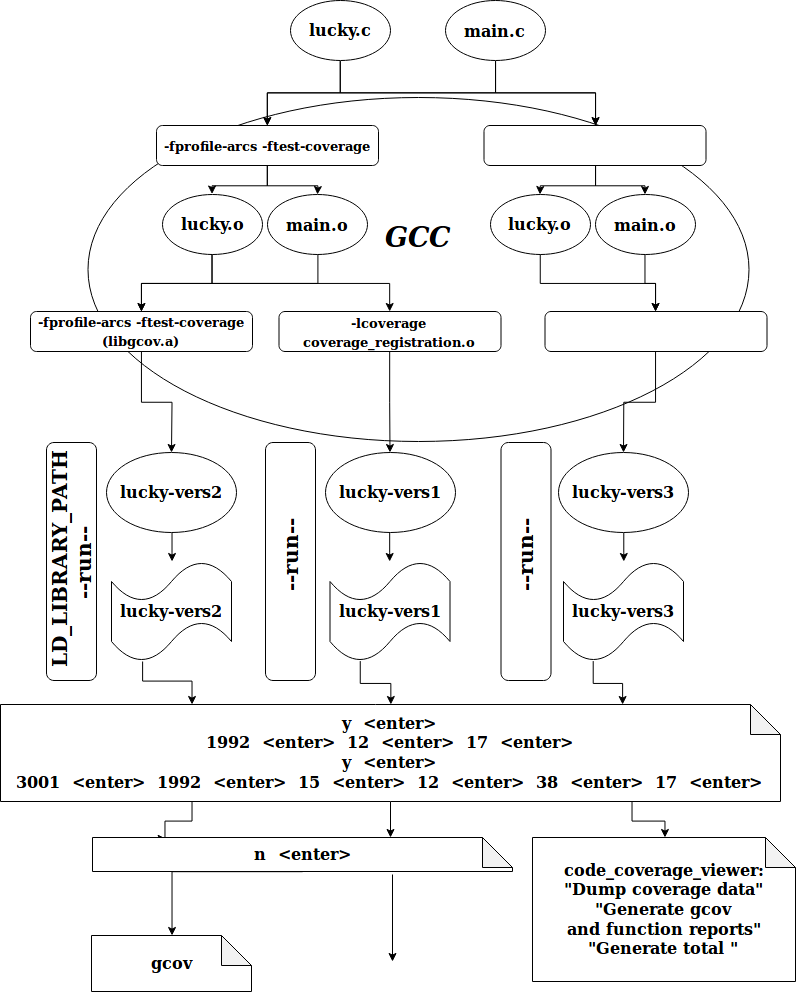
\includegraphics[width=\textwidth , height=0.9\textheight]{img/lucky_diagram.png}
  \caption{Plan testiranja instrumentalizacije programa \strano{lucky}}
  \label{fig:diag}
\end{figure}

\subsubsection{Sprovođenje testiranja i analiza rezultata}

Pre početka testiranja, neophodno je kreirati radno okruženje, sledećim naredbama:
\begin{enumerate}
\item kreiranje radnog direktorijuma: \\
\kod{mkdir test\_workspace}
\item kreiranje tri bazna direktorijuma sa kodom za različite verzije programa: \\
\kod{mkdir test\_workspace/version\_01} \\
\kod{mkdir test\_workspace/version\_02} \\ 
\kod{mkdir test\_workspace/version\_03} \\
\kod{cp lucky.c main.c test\_workspace/version\_01} \\
\kod{cp lucky.c main.c test\_workspace/version\_02} \\
\kod{cp lucky.c main.c test\_workspace/version\_03} 
\item kreiranje direktorijuma sa bibliotekom \strano{libcoverage} i registratorom signala: \\
\kod{mkdir test\_workspace/runtime\_coverage} \\
\kod{cp libcoverage.so test\_workspace/runtime\_coverage} \\
\kod{cp coverage\_registration.o test\_workspace/runtime\_coverage} \\ 
\kod{cp code\_coverage\_viewer.py test\_workspace/runtime\_coverage}
\end{enumerate}

Prvi korak testiranja obuhvata prevođenje programa na tri načina. Objektni i izvršni fajlove smeštaju se u odgovarajući radni direktorijum konkretne verzije. Za potvrdu uspešnosti ovog koraka, proverava se prisustvo fajlova gcno, komandom \kod{ls} i prisustvo funkcija: \kod{\_\_gcov\_init}, \kod{gcov\_exit} i \kod{drew\_coverage}, komandom \kod{readelf}. Dobijeni rezultati obuhvataju:
\begin{enumerate}
\item prisustvo fajlova: \strano{main.gcno} i \strano{lucky.gcno} isključivo u direktorijumima instrumentalizovanih verzija
\item prisustvo funkcija \kod{\_\_gcov\_init} i \kod{drew\_coverage} i odustvo funkcije \kod{gcov\_exit} u programu \strano{lucky-vers3}
\item prisustvo funkcija \kod{\_\_gcov\_init} i \kod{gcov\_exit} i odustvo funkcije \kod{drew\_coverage} u programu \strano{lucky-vers2}
\item odsustvo funkcija \kod{\_\_gcov\_init}, \kod{drew\_coverage} i \kod{gcov\_exit} u programu \strano{lucky-vers1}
\end{enumerate}

\noindent što predstavlja ispravne rezultate. Sprovođenje prvog koraka testiranja i rezultati istog, prikazani su na slici \ref{fig:lucky-test-1}.

\begin{figure}[!ht]
  \centering
  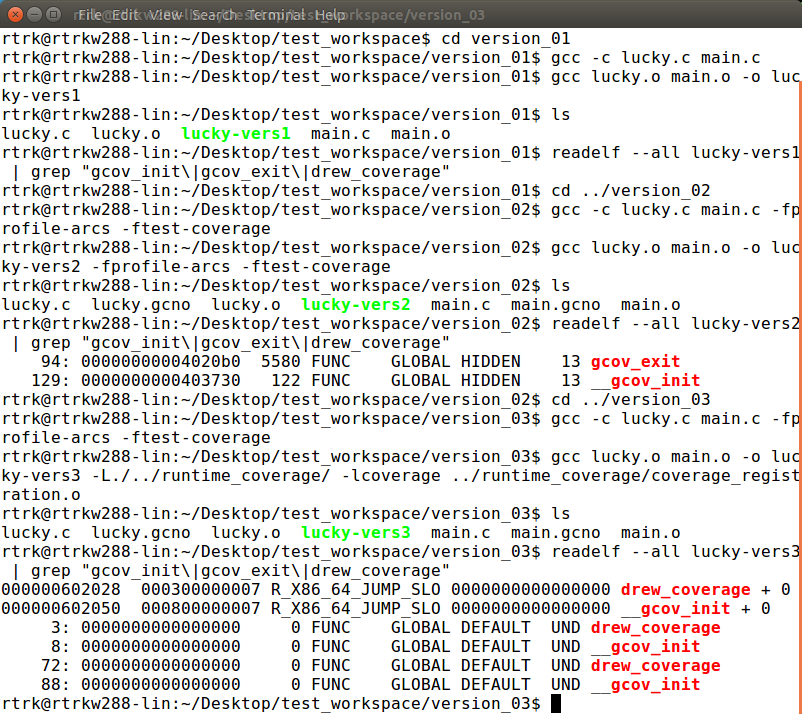
\includegraphics[width=\textwidth]{img/lucky1-ng.png}
  \caption{Testiranje na programu \strano{lucky} - Korak 1}
  \label{fig:lucky-test-1}
\end{figure}

Drugi korak obuhvata pokretanje sva tri programa u tri različita terminala, kako bi se omogućila komunikacija putem standardnog ulaza/izlaza. Za pokretanje trećeg programa, bilo je neophodno uključiti i adresu biblioteke \strano{libcoverage.so} u promenljivu okruženja \strano{LD\_LIBRARY\_PATH}, kako bi se linker informsao gde je treba potražiti. Prikaz drugog koraka je dat na slici \ref{fig:lucky-test-2}. 

\begin{figure}[!ht]
  \centering
  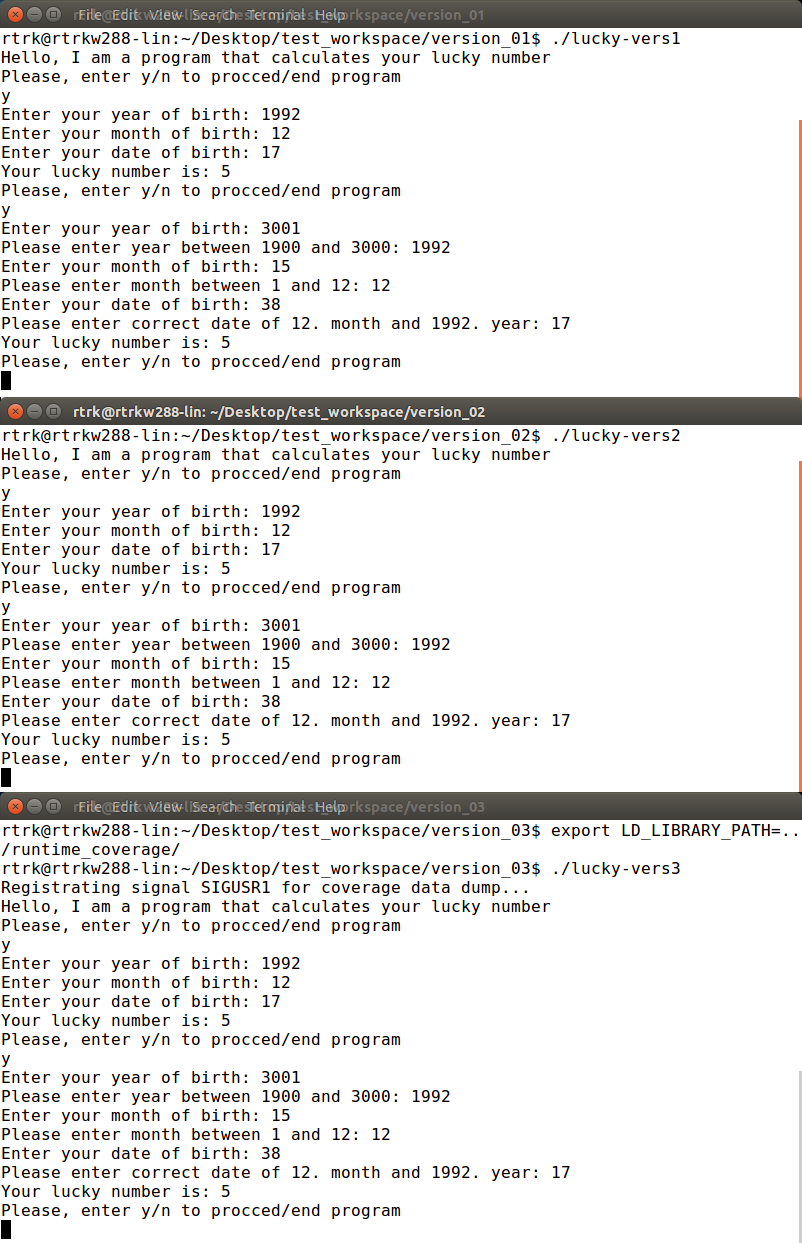
\includegraphics[width=0.88\textwidth]{img/lucky2-ng.png}
  \caption{Testiranje na programu \strano{lucky} - Koraci 2 i 3}
  \label{fig:lucky-test-2}
\end{figure}

Za izvršavanje trećeg koraka testranja, bilo je potrebno definisati jedan slučaj upotrebe programa \strano{lucky}. U cilju što bolje demostracije pojma pokrivenosti i razlika starog i novog pristupa prikupljanju podataka iz izvršavanja programa, odabran je skup komandi koji rezultuju visokoj pokrivenosti. Rezultati ovog koraka prikazani su na slici \ref{fig:lucky-test-2}. i na osnovu njih se može zaključiti da do ovog trenutka nema razlika u ponašanju između različitih verzija programa, što je jedna od glavih odlika ispravne instrumentalizacije. 

Naredni korak predstavlja najbitniji korak testiranja. Materijal generisan u ovom koraku predstavlja krajnji proizvod i njegove karakteristike će učestvovati u procesu finalne validacije. Procedura se razlikuje u zavisnosti od verzije programa. Izvršavanje neinstrumentalizovane verzije, više nije neophodno, te se ista prekida odabirom opcije: n. Program, čije podatke iz izvršavanja prikuplja standardna biblioteka \strano{libgcov}, će automatski izvršiti ispis tih podataka na kraju izvršavanja, stoga se i njegovo izvršavanje prekida na isti način. Važno je napomenuti da u slučaju nasilnog prekida programa, poput prekida korišćenjem signala \strano{SIGKILL} ili \strano{SIGARBT}, funkcija \kod{atexit} se neće izvršiti i fajlovi \strano{gcda} neće biti generisani. Stoga se može jasno zaključiti da se podaci o pokrivenosti koda programa koji nemaju ugrađeni mehanizam za takozvani: “graciozni izlaz” mogu dobiti samo i isključivo korišćenjem nove biblioteke \strano{libcoverage}. U trenutnom test primeru nije prisutno tako nešto, zbog čega su fajlovi \strano{gcda} uspešno generisani i neprazni. Pozivom alata \strano{gcov}, generišu se uspešno izveštaji, koji će se validirati u narednom koraku. Rezultati koraka 4.a i 4.b prikazani su na slici \ref{fig:lucky-test-3}.

\begin{figure}[!ht]
  \centering
  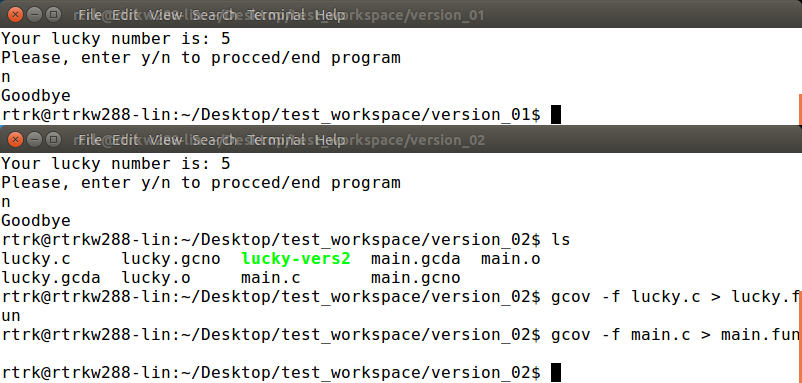
\includegraphics[width=\textwidth]{img/lucky3-ng.png}
  \caption{Testiranje na programu \strano{lucky} - Koraci 4.a i 4.b}
  \label{fig:lucky-test-3}
\end{figure}

Program \strano{lucky-vers3} se ne prekida odmah, već se najpre vrši kreiranje fajlova gcda i izveštaja. Pokreće se \strano{code\_coverage\ viewer} i nakon pritiska na dugme: \strano{Choose workspace} odabira se radni direktorijum: \strano{test\_workspace/version\_03}. U tekstualno polje za unos imena programa, unosi se: \strano{lucky-vers3}, a zatim inicira signal za poziv funkcije \kod{drew\_coverage} klikom na dugme \strano{Dump coverage data}, a uspešnost ovog dela procedure može se lako potvrditi postojanjem nepraznih fajlova gcda u radnom direktorijumu. Dugme: \strano{Generate gcov and fun files} pokreće kreiranje izveštaja, čija imena smešta u drvoliku komponentu, dok se sadržaj selektovanog izveštaja prikazuje u desnoj polovini ekrana. Slika \ref{fig:lucky-test-4} vizuelno demonstrira rezultate ovog koraka.

\begin{figure}[!ht]
  \centering
  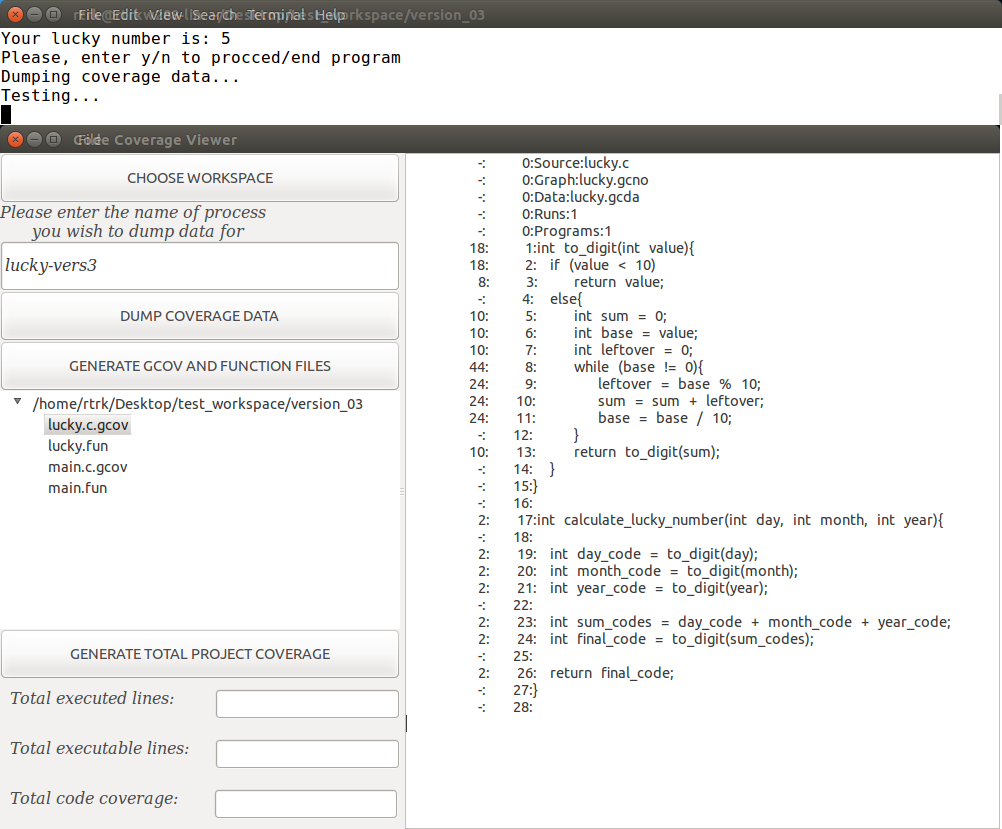
\includegraphics[width=\textwidth]{img/lucky4-ng.png}
  \caption{Testiranje na programu \strano{lucky} - Korak 4c}
  \label{fig:lucky-test-4}
\end{figure}

Poslednji korak testiranja obuhvata analizu i validaciju rezultata prethodnih koraka. 

Na slici \ref{fig:lucky-test-5}. prikazan je ispis programa: \strano{lucky-vers1}, \strano{lucky-vers2} i \strano{lucky-vers3} na standardni izlaz. U sva tri slučaja ispis iz inicijalnog dela slučaja upotrebe, odnosno zaključno sa poslednjom porukom sadržaja: \strano{Your lucky number is: 5}, je identičan. Time je zadovoljen prvi kriterijum validacije ispisa, odnosno regularnost izvršavanja programa tokom instrumentalizacije. Ispis programa \strano{lucky-vers3} ne sadrži oproštajnu poruku: \strano{Goodbye}, već samo ispise iz registarora i biblioteke, čime su zadovoljena i preostala dva kriterijuma validnosti ispisa. 

\begin{figure}[!ht]
  \centering
  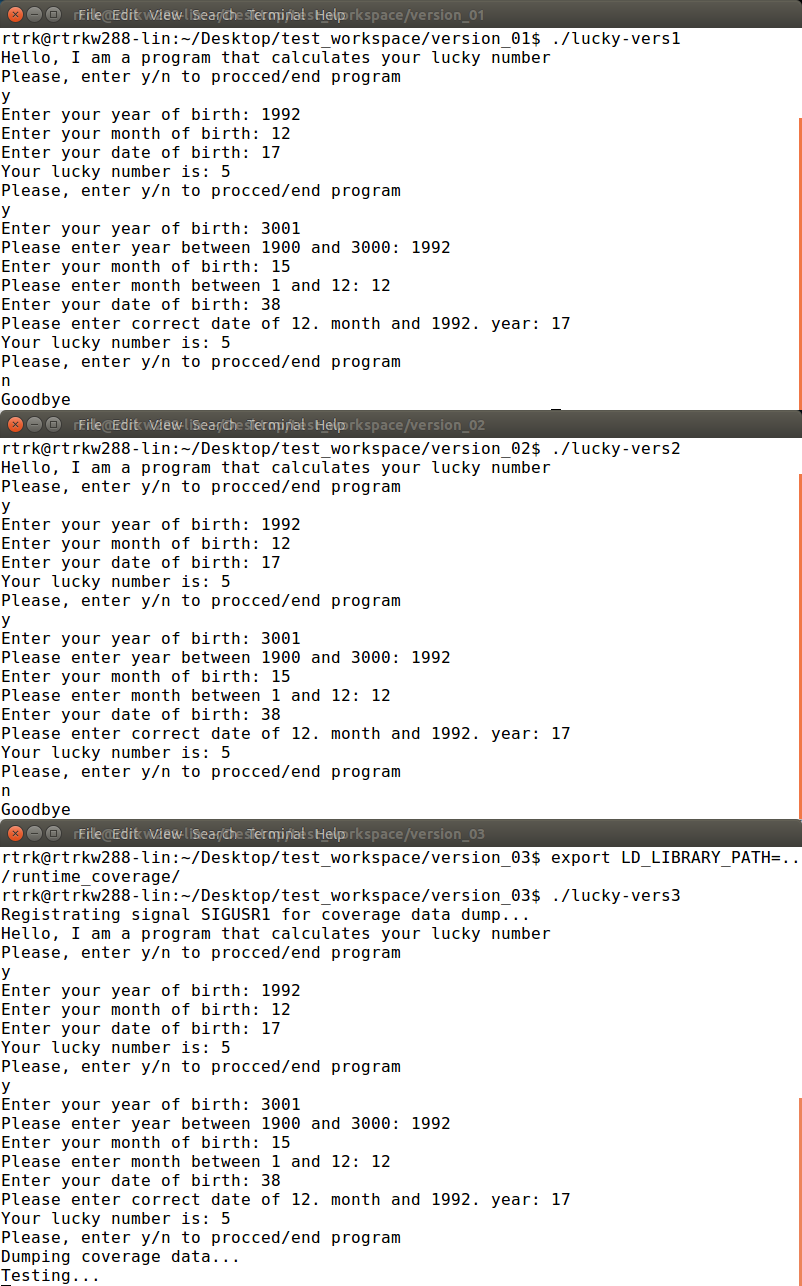
\includegraphics[width=0.85\textwidth]{img/lucky5-ng.png}
  \caption{Testiranje na programu \strano{lucky} - Korak 5a}
  \label{fig:lucky-test-5}
\end{figure}

Zajedničkom analizom koda i ispisa različitih verzija programa \strano{lucky}, mogu se izvesti očekivane vrednosti za izveštaje. Celokupni kod fajla izvornog koda: \strano{lucky.c} se izvršava identičan broj puta u sva tri slučaja. Prikupljanje podataka statičkom bibliotekom \strano{libgcov} se aksiomatski uzima za ispravno, kao sastavni dao programskog prevodioca \strano{GCC}. Usled toga se jednom potvrdom ispravnog prikupljanja podataka novom bibliotekom može smatrati jednakost izveštaja: \\ \strano{test\_workspace/version\_02/lucky.c.gcov} i \strano{test\_workspace/version\_03/lucky.c.gcov}, odnosno: \\
\strano{test\_workspace/version\_02/lucky.fun} i \strano{test\_workspace/version\_03/lucky.fun}  \\
Linux komandom \strano{diff} ili jednostavnim posmatranjem može se potvrditi da je kriterijum jednakosti ispunjen, što je vizuelno prikazano na slici \ref{fig:lucky-test-6}.

\begin{figure}[!ht]
  \centering
  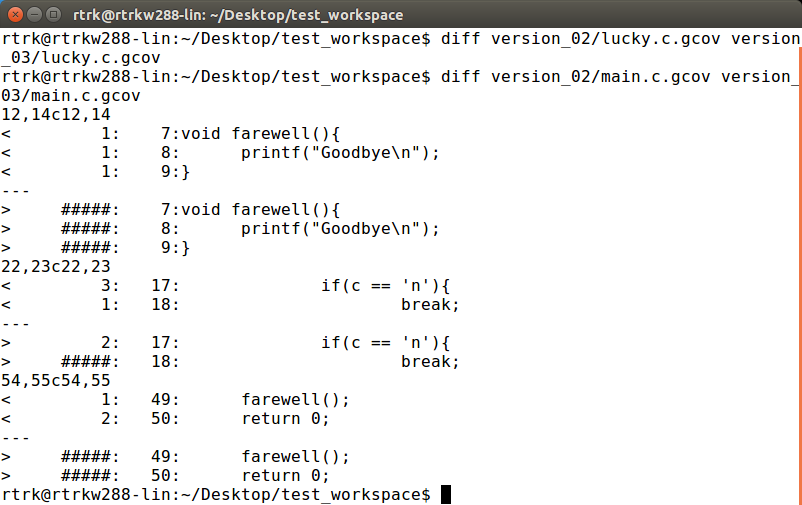
\includegraphics[width=\textwidth]{img/lucky6-ng.png}
  \caption{Testiranje na programu \strano{lucky} - Korak 5b}
  \label{fig:lucky-test-6}
\end{figure}

Sa druge strane, izveštaji za fajl izvornog koda: \strano{main.c}, moraju se razlikovati tačno za poslednju iteraciju u okviru najveće petlje i za po jedan poziv funkcija \kod{farewell} and \kod{return}. Na slici \ref{fig:lucky-test-5}, na kojoj je prikazan izlaz komande \strano{diff} i za ova dva \strano{gcov} izveštaja, jasno se vidi da su ta očekivanja ispunjena. 

Pristup koji je trenutno implementiran u okviru prevodioca \strano{GCC} nema ugrađenu podršku za računanje ukupne pokrivenosti. Stoga će se ova funkcionalnost testirati nezavisno od tradicionalnog pristupa, poređenjem rezultata interfejsa \\ \strano{code\_coverage\_viewer} sa manuelno izračunatim vrednostima. Jednostavnim prebrajanjem dobijaju se vrednosti u skladu sa onima koje je prikazao \\ \strano{code\_coverage\_viewer}, koje se mogu videti i na slici \ref{fig:lucky-test-7}

\begin{figure}[!ht]
  \centering
  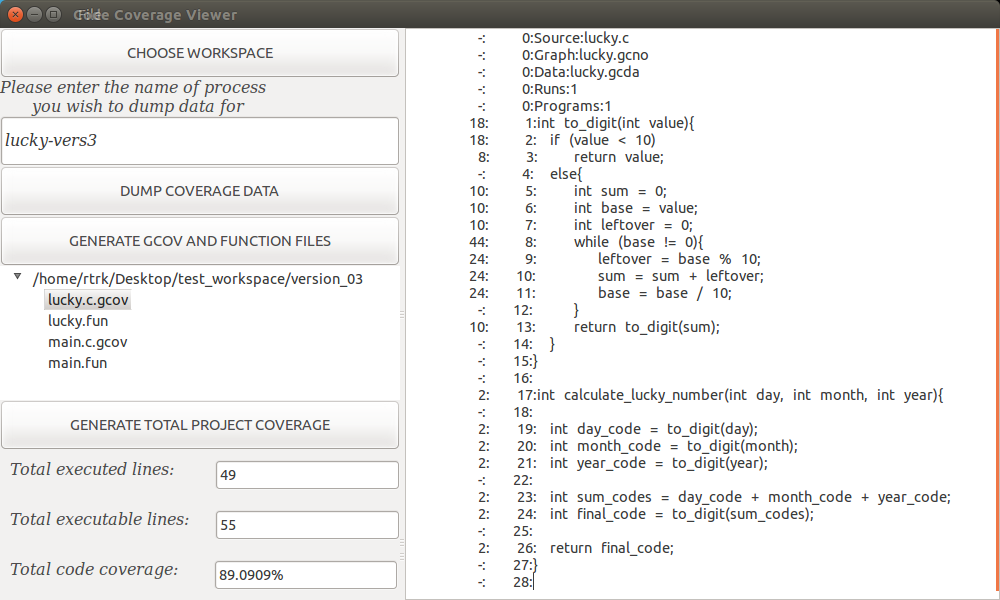
\includegraphics[width=\textwidth]{img/lucky7-ng.png}
  \caption{Testiranje na programu \strano{lucky} - Korak 5c}
  \label{fig:lucky-test-7}
\end{figure}

Svi koraci plana za testiranje, definisanog na početku ove sekcije, su dakle ispunjeni, pa se testiranje može proglasiti uspešno obavljenim. 


\subsection{Kompleksni primer: QEMU}

Za demonstraciju korektnosti rada biblioteke \strano{libcoverage} i grafičkog korisničkog interfejsa \strano{code\_coverage\_viewer} u realnim situacijama odabran je projekat \strano{QEMU}, najpre zbog svoje veličine i značaja, ali i zbog karakteristika na kojima se mogu dobro sagledavati različite prepreke koje se mogu javiti prilikom infiltracije novog softverskog rešenja za prikupljanje podataka iz izvršavanja u realni projekat, kao i načini za njihovo prevazilaženje.

\subsubsection{Šta je QEMU}

\strano{QEMU} je slobodni softver otvorenog koda, čija osnovna funkcija predstavlja emuliranje operativnih sistema ili programa na mašini različite arhitekture od njih samih. Spektar podržanih arhitektura na kojima se \strano{QEMU} može pokrenuti ili koje može emulirati je veoma širok, i obuhvata \strano{MIPS}, \strano{ARM}, \strano{x86}, \strano{PPC} i mnoge druge.
\strano{QEMU} ima dva režima rada:
\begin{enumerate}
\item sistemski: potpuna emulacija jednog sistema (npr. operativnog) na drugom
\item korisnički (samo za linux): emulacija izvršavanja jedinstvenog procesa, prevedenog za jednu arhitekturu, na mašini druge arhitekure.
\end{enumerate}
Za potrebe ovog testiranja, instrumentalizovaće se kompletni kod \strano{QEMU}-a, ali će pokretanje biti ograničeno na dva programa korisničkog režima koji simuliraju rad \strano{MIPS} i \strano{ARM} procesora.

\subsubsection{Opis koda i kako radi \strano{QEMU}}

Osnovni radni direktorijum \strano{QEMU}-a sadrži veliki broj skripti za definisanje fleksibilnih parametara, \strano{makefile}-ova sa instrukcijama za izgradnju sistema i fajlova izvornog koda pisanih u programskom jeziku C. Skripte za konfiguraciju, osnovni \strano{makefile}-ovi i kodovi pojedenih alata su smešteni u sam koreni direktorijum projekta. Ostatak je grupisan u poddirektorijume prema funkcionalnosti i/ili programu kome pripadaju.

Glavni deo koda programa koji čine sistemski režim rada se nalazi u poddirektorijuma čiji nazivi sadrže ime arhitekture koja se emulira i sufiks \strano{-softmmu}. U njega se smešta i izvršna verzija, prepoznatljiva po prefiksu: \strano{qemu-system-}.

Poddirektorijumi čiji nazivi sadrže ime arhitekture i sufiks \strano{-linux-user}, sadrže osnovni deo koda odgovarajćeg programa korisničkog režima koji emulira tu arhitekturu. Prevođenjem se kreira izvršna verzija, koja se smešta u isti direktorijum, i čiji naziv sačinjavaju prefiks \strano{qemu-} i naziv arhitekture emuliranog programa.

Proces kreiranja izvršnih programa u okviru \strano{QEMU} projekta se sastoji iz dva koraka:
\begin{enumerate}
\item konfigurisanje parametara za prevođenje
\item prevođenje izvornog koda programa projekta \strano{QEMU} sa tako konfigurisanim parametrima
\end{enumerate}
Za izvođenje prvog koraka zadužena je \strano{shell} skripta, pod nazivom \strano{configure}, koja se nalazi u osnovnom radnom direktorijumu. Podrazumevana konfiguracija se kreira pozivom bez dodatnih opcija. Redefinisanje svakog parametra prevođenja je uslovljeno prisustvom odgovarajuće opcije tokom poziva skripte. Nove vrednosti se upisuju u konfiguracione fajlove koji se takođe nalaze u korenom direktorijumu projekta i koriste kasnije tokom prevođenja. Na ovaj način se može izmeniti programski prevodilac (\kod{--cc=CC}), omogućiti prevođenje sa dodatnim flegovima (\kod{--extra-cflags=CFLAGS}), odabrati skup programa za prevođenje i slično. Opcija koja je ce biti naročito važna u ovom testiranju je: \kod{--enable-gcov} koja uslovljava instrumentalizaciju uz prikupljanje podataka standardnom bibliotekom \strano{libgcov}.

Pravila za izgradnju svih programa i alata u sklopu \strano{QEMU} projekta su definisana mrežom \strano{makefile}-ova, pri čemu je raspoređivanje izvršeno po kriterijumima pripadnosti i/ili funkcionalnosti. Proces prevođenja se pokreće ključnom rečju \strano{make}. Predefinisano ponašanje podrazumeva izgradnju maksimalnog skupa programa i alata, ali se on po želji može i redukovati korišcenjem određenih opcija prilikom konfigurisanja, u cilju uštede vremena.

\subsubsection{Ograničenja i prilagođavanja}

Za razliku od jednostavnog primera kao što je program za računanje srećnog broja, sistem pravila za prevođenje, kao i sam kod \strano{QEMU}-a su znatno složeniji. Stoga je i implementacija podrške za prikupljanje i prikaz podataka u toku izvršavanja iziskivala veći stepen prilagođavanja i kvantitet izmena. 

Prva iteracija je obuhvatala izmene prevođenja, odnosno dodavanje flegova za instrumentalizaciju, biblioteke \strano{libcoverage} i objektnog fajla \strano{coverage\_registration.o}. 
Očekivana složenost ovog procesa u slučaju prosečnog, većeg projekta, je izrazito velika, iz razloga što zahteva poznavanje sistema za izgradnju softvera do najsitnijih detanja. Za prilagođavanje softvera digitalne televizije, na kojima je biblioteka \strano{libcoverage} originalno testirana, bilo je potrebno više nedelja rada, kao i asistencija stručnjaka za njihove sisteme izgradnje. Međutim, planski i ciljani odabir upravo \strano{QEMU}-a za ovo testiranje, je dosta redukovao vreme potrebno za prvu iteraciju prilagođavanja. Već ugrađena podrška za staitičku instrumentalizaciju na kraju izvršavanja je poslužila kao dobar šablon za oponašanje, koji je nadomestio nedostatak poznavanja sistema. 

Po ugledu na opciju: \kod{--enable gcov}, u skriptu za konfigurisanje je uvedena nova opcija: \kod{--enable-runtime-gcov}, koja takođe uslovljava uključivanje flegova za instrumentalizaciju u toku prevođenja izvornog fajla do objektnog, ali u proces linkovanja umesto njih uslovljava prisustvo dinamičke biblioteke \strano{libcoverage} i objektnog fajla za registraciju signala. Ispisivanje odgovarajućih vrednosti u konfiguracioni fajl: \strano{config\_host.mak} urađen je identično kao u slučaju postojeće opcije \kod{--enable gcov}. 

Korišćenje istih vrednosti u konfiguracionom fajlu je znatno uticalo na olakšavanje implementacije i validnost procesa instrumentalizacije uz primenu nove biblioteke, ali i proizvelo potrebu za razlikovanjem starog i novog pristupa prikpljanja podaka iz izvršavanja na nivou fajlova izvornog koda. Razlog predstavlja prisustvo koda u okviru fajla \strano{linux-user/exit.c}, koji koristi funkciju standardne biblioteke \strano{libgcov} da proširi mogućnost instrumentalizacije na neke slučajeve neregularnih izlazaka iz programa. Razlikovanje na nivou fajlova izvornog koda ostvareno je uvođenjem nove promenljiva \kod{RUNTIME\_GCOV}, koja se, u slučaju novog pristupa, prosleđuje zajedno sa instrumentalizacionim flegovima u toku prevođenja izvornog fajla do objektnog korišćenjem opcije \kod{–D}. Korišćenje funkcije standardne biblioteke \strano{libgcov} je uslovljeno nedefinisanošću ove promenljive. Kompletne izmene skripte \strano{configure} u git formatu, prikazane su na listingu \ref{qemu-diff-1}. Izmene fajla \strano{linux-user/exit.c} u kojima se uvodi korišćenje promenljive \kod{RUNTIME\_GCOV}, prikazane su na listingu \ref{qemu-diff-2}. \\

\begin{lstlisting}[caption={Izmene skripte \strano{configure}},frame=single, label=qemu-diff-1]
diff --git a/configure b/configure

@@ -389,6 +389,7 @@ tcg_interpreter="no"
 gcov="no"
+runtime_gcov="no";
 gcov_tool="gcov"

@@ -1002,6 +1003,8 @@ for opt do
   ;;
+  --enable-runtime-gcov) runtime_gcov="yes"
+  ;;
   --static)

@@ -1676,6 +1679,7 @@ Advanced options 
   --enable-gcov            enable test coverage analysis with gcov
+  --enable-runtime-gcov     enable runtime coverage analysis with gcov
   --gcov=GCOV              use specified gcov [$gcov_tool]

@@ -5675,6 +5679,10 @@ write_c_skeleton
   LDFLAGS="-fprofile-arcs -ftest-coverage $LDFLAGS"
+elif test "$runtime_gcov" = "yes" ; then
+  CFLAGS="-fprofile-arcs -ftest-coverage -g -DRUNTIME_GCOV $CFLAGS"
+  LDFLAGS="-L\$(BUILD_DIR)/code_coverage_lib -lcoverage $LDFLAGS"
+  LDFLAGS="\$(BUILD_DIR)/code_coverage_lib/coverage_registration.o $LDFLAGS"
 elif test "$fortify_source" = "yes" ; then
 
@@ -6128,6 +6136,7 @@ echo "crypto afalg      
 echo "gcov enabled      $gcov"
+echo "runtime gcov enabled $runtime_gcov"
 echo "TPM support       $tpm"

@@ -7023,6 +7032,11 @@ if test "$gcov" = 
 fi
+if test "$runtime_gcov" = "yes" ; then
+  echo "CONFIG_GCOV=y" >> $config_host_mak
+  echo "GCOV=$gcov_tool" >> $config_host_mak
+fi
+
if test "$docker" != "no"; then
\end{lstlisting}

\newpage
\begin{lstlisting}[caption={Izmene fajla \strano{linux-user/exit.c}},frame=single, label=qemu-diff-2]
diff --git a/linux-user/exit.c b/linux-user/exit.c

@@ -19,17 +19,22 @@
 #include "qemu.h"
+#ifndef RUNTIME_GCOV
 #ifdef CONFIG_GCOV
 extern void __gcov_dump(void);
 #endif
+#endif
 
 void preexit_cleanup(CPUArchState *env, int code)
 {
 #ifdef TARGET_GPROF
         _mcleanup();
 #endif
+
+#ifndef RUNTIME_GCOV
 #ifdef CONFIG_GCOV
         __gcov_dump();
 #endif
+#endif
         gdb_exit(env, code);
\end{lstlisting}

Testiranjem funkcionalnosti implementirane u toku prve iteracije, detektovana je prva smetnja u ispravnom radu podrške za prikupljanje i prikaz podataka u toku izvršavanja. Detaljnom analizom je utvrđeno da se uprkos uspešnoj registraciji funkcije \kod{coverage\_handler} kao \strano{signal-handler}-a za \strano{SIGUSR1}, k\^{o}d unutar te funkcije ne izvršava. Uzrok ove pojave je predfinisanje svih signala u kodu korisničkih emulatora \strano{QEMU}-a. Kako bi obezbedio emulaciju maksimalnog kvaliteta koja uključuje i podršku za slanje i prijem \strano{POSIX} signala, sve primljene signale \strano{QEMU} prosleđuje emuliranom korisničkom programu. Poruka karakteristična za signal \strano{SIGUSR1}, koja je ispisana tokom testiranja rezultata prve iteracije, nije dakle vodila poreklo iz \strano{QEMU}-a već iz emuliranog korisničkog programa. U cilju prevazilaženja ove prepreke, sprovedena je druga iteracija implementacije podrške za prikupljanje i prikaz podataka u toku izvršavanja, u okviru koje je osmišljen i realizovan novi algoritam za prijem i obradu signala instrumentalizovane verzije \strano{QEMU}-a. 

Promena konkretnog signala ne bi proizvela drugačije rezultate, usled maksimalne pokrivenosti mehanizma prosleđivanja, dok bi promena tehnike komunikacije sa procesima isuviše negativno uticala na vreme i složenost razvoja. Stoga je potraga za rešenjem okrenuta ka kodu \strano{QEMU}-a. Sprovedena je nova analiza dokumentacije i izvornog koda, tokom koje je izvršena lokalizacija funkcije za prijem i obradu signala i utvrđen mehanizm njenog rada. Definisanje jedinstvenog \strano{signal-handlera} za sve signale, pod nazivom: \kod{host\_signal\_handler}, obavlja se u fajlu izvornog koda: \strano{linux-user/signal.c}. 

Inicijalni plan ugrađivanja podrške za pokretanje prikupljanja podataka iz izvršavanja \strano{POSIX} signalom, podrazumevao je bezuslovnu modifikaciju ponašanja uslovljenog prijemom signala \strano{SIGUSR1} u okviru funkcije \strano{host\_signal\_handler}. Razmatran je zbog svoje jednostavnosti i lakoće implementacije. Međutim, usled nemogućnosti pravilnog razlikovanja upotebe signala \strano{SIGUSR1} kao okidača prikupljanja podataka o pokrivenosti i slučaja kada ga treba prosledti emuliranom programu, nastala je potreba za dodatnim usavršavanjem. 
Na formiranje nove ideje uticalo je posmatranje argumentata funkcije \kod{host\_signal\_handler}, tačnije onog argumenta koji predstavlja instancu strukture \kod{siginfo\_t}. 

U okviru zaglavlja \strano{signal.h}, nalazi se više funkcija koje se mogu koristiti za slanje signala. Jednostavniji od ponuđenih mehanizama, slanje signala bez dodatnih informacija funkcijom \kod{kill}, implementiran je u okviru interfejsa \strano{code\_coverage\_viewer} kao rešenje koje zadovoljava očekivane funkcionalne zahteve. Sa druge strane, u cilju mogućnosti emuliranja potpuno proizvoljnog programa, koji može komunicirati i naprednijim mehanizmom, slanjem signala sa dodatnim informacijama funkcijom \kod{sigqueue}, trenutna implementacija \strano{QEMU}-a sadrži ugrađenu podršku i za prosleđivanje poruke poslate sa signalom. Sadržaj poruke je predstavljen jedinstvenom celobrojnom vrednošću i/ili pokazivačem na strukturu u memoriji proizvoljnog tipa, a čuva se posebnom polju strukture tipa \kod{siginfo\_t}: uniji \kod{sigval}. Korisnički emulatori \strano{QEMU}-a u regularnom slučaju ne vrše čitanje i obradu nijedne informacije po prijemu signala, što pruža dovoljan prostor za nadogradnju \strano{signal-handler}-a u fazi između prijema i prosleđivanja. Pozitivna vrednost promenljive \kod{RUNTIME\_GCOV}, koja se prosleđuje prilikom prevođenja u slučaju instrumentalizacije novim pristupom, uslovljava čitanje vrednosti broja signala i prateće poruke i dodatnu akciju u slučaju predefinisane kombinacije za prikupljanje podataka iz izvršavanja: signal \strano{SIGUSR1} i tajna poruka: 45949. Specijalna celobrojna vrednost 45949 je dobijena iz poruke \kod{call drew\_coverage} kombinacijom \strano{md5} algoritma za heširanje i osnovnih aritmetičkih operacija. Kompletne izmene koda \strano{QEMU}-a u sklopu druge iteracije implementacije, prikazane su, u git formatu, na listingu \ref{qemu-diff-3}.

\newpage

\begin{lstlisting}[caption={Izmene fajla \strano{linux-user/signal.c}} ,frame=single, label=qemu-diff-3]
diff --git a/linux-user/signal.c b/linux-user/signal.c

@@ -642,6 +642,10 @@ static inline void rewind_if_in_safe_syscall(void *puc)
 #endif
+#ifdef RUNTIME_GCOV
+extern void coverage_handler(int signo);
+#endif
+
 static void host_signal_handler(int host_signum, siginfo_t *info,
                                 void *puc)

@@ -666,6 +670,24 @@ static void host_signal_handler(int host_signum, siginfo_t *info,
         return;
+
+     
+     int message_int = info->si_value.sival_int;
+     printf("Recieved signal: %d with message: %d\n",host_signum, message_int);
+     //Checking if signal and message corespond to predefind coverage dumping comunication
+     if (host_signum == SIGUSR1 && message_int == 45949){
+#ifdef RUNTIME_GCOV
+       // informing about begining of coverage dump procedure and invoking coverage handler that will do the dumping
+	printf("Program %s is about to dump coverage data\n", program_invocation_short_name);
+	coverage_handler(host_signum);
+       //Informing about end of coverage dump procedure
+	printf("Program %s has finished dumping coverage data\n", program_invocation_short_name);
+	// reseting value of message since it is alredy being processed.
+	info->si_value.sival_int = 0;
+	return;
+#endif
+    }
+
     trace_user_host_signal(env, host_signum, sig);
\end{lstlisting}

Prednost u odnosu na inicijalni plan se ogleda u znatnoj redukciji ograničenja mogućnosti instrumentalizovane verzije emulatora. Gornje ograničenje broja različitih signala je značajno manje od maksimalne celobrojne vrednosti koja se može smestiti u promenljivu tipa \kod{int}. Pored toga, verovatnoća slučaja upotrebe emuliranja korisničkog programa koji koristi tačno ovu kombinaciju je znatno manja nego u slučaju bezuslovne upotrebe signala \strano{SIGUSR1}. Iznimno, podaci iz izvršavanja su ipak namenjeni i potrebni isključivo razvijaocima \strano{QEMU} projekta. Stoga i ako dođe do pojave ekstremnog slučaja upotrebe na koga utiče ovo minimalno ograničenje, razvojni tim poseduje dovoljno znanja i iskustva da promeni korišćeni signal i/ili poruku. \\

\begin{lstlisting}[caption={Kod u okviru fajla \strano{messanger.c}} ,frame=single, label=qemu-diff-4]
#include <stdio.h>                                                       
#include <signal.h>                                                      
#include <unistd.h>     
#include <stdlib.h>
static int pid;
void message_handler(int signo){
    if (signo==SIGUSR1){
	printf("Sending signal to pid %d to dump data\n", pid);   
	union sigval coverage_code;
        coverage_code.sival_int = 45949;
        sigqueue(pid, SIGUSR1, coverage_code);
    }
}
int main(int argc, char**argv){
	if(argc == 2) {
		pid = atoi(argv[1]);
		printf("Registrating signal SIGUSR1 for passing message 45949 to pid: %d...\n",pid);
		signal(SIGUSR1,message_handler);
		while(1){}
	}
	else{
		printf("Incorrect number of command line arguments. Passing %d instead of 1.\n", argc-1);
		printf("Please pass a single number as argument that presents the PID of target process.\n");
	}
	return 0;
}
\end{lstlisting}


Izmenom okidača za ispis podataka iz izvršavanja u fajlove gcda, došlo je do nekompatibilnosti interfejsa \strano{code\_coverage\_viewer} i programa instrumentalizovane verzije \strano{QEMU} skupa emulatora. 

Prevazilaženje ove prepreke ostvareno je kreiranjem posredničkog programa, sa ulaznim interfejsom kompatibilnim mehanizmu strano{code\_coverage\_viewer}-a, odnosno prijemu signala bez poruke, i izlaznim interfejsom kompatibilnim \strano{QEMU}-u, odnosno slanju signala sa porukom. Program nosi naziv: \strano{messanger}, što simbolizuje njegovu ulogu glasnika između novog grafičkog interfejsa i \strano{QEMU}-a. 

Program messanger se pokreće sa jednim argumentom komandne linije koji predstavlja identifikator instrumentalizovanog pokrenutog \strano{QEMU} emulatora kome treba preneti poruku. Nakon registracije \strano{signal-handler}-a za \strano{SIGUSR1}, \strano{messanger} prelazi u stanje čekanja. Po prijemu odgovarajućeg signala, emituje se signal sa porukom 45494, koji uslovljava poziv funkcije \kod{drew\_coverage} u emulatoru sa identifikatorom iz argumenta komandne linije. Kod posredničkog programa, pisan u programskom jeziku C, prikazan je na listingu \ref{qemu-diff-4}.

Nakon uspešnog okončavanja druge iteracije implementacije podrške za prikupljanje i prikaz podataka u toku izvršavanja u okviru projekta \strano{QEMU}, stvorili su se optimalni uslovi za finalno testiranje. 

\subsubsection{Plan testiranja}

Finalno testiranje biće sprovedeno nad dva \strano{QEMU} emulatora koja rade u korisničkom režimu:
\begin{enumerate}
\item \strano{mips-linux-user/qemu-mips}
\item \strano{arm-linux-user/qemu-arm}
\end{enumerate}
Za program koji će emulirati sve verzije, odabrana je neistrumentalizovana verzija programa \strano{lucky}, detaljnije opisana u prethodnoj sekciji.
Za potrebe testiranja, biće kreirane tri verzije \strano{QEMU} skupa emulatora:
\begin{enumerate}
\item \strano{<qemu\_vers1>/qemu/<arch>-linux-user/qemu-<arch>} bez instrumentalizacije
\item \strano{<qemu\_vers2>qemu/<arch>-linux-user/qemu-<arch>} sa instrumentalizacijom i standardnom bibliotekom \strano{libgcov}
\item \strano{<qemu\_vers3>qemu/<arch>-linux-user/qemu-<arch>} sa instrumentalizacijom i novom bibliotekom \strano{libcoverage}.
\end{enumerate}
Plan za testiranje je definisan sledećim koracima:
\begin{enumerate}

\item konfiguracija i prevođenje:
\begin{enumerate}
\item verzija bez instrumentalizacije se konfiguriče sa opcijom \kod{–enable-debug} kako bi se postigao isti stepen optimizacije sa instrumentalizovanim verzijama: \\ \kod{./configure –enable-debug}\\ dodavanje ove opcije ne utiče na izvršavanje, već je značajno samo za poređenje memoriske zahtevnosti verzija
\item verzija sa instrumentalizacijom i standardnom bibliotekom \strano{libgcov} se konfiguriše sa starom opcijom za instrumentalizaciju: \\
\kod{./configure –enable-gcov}
\item verzija sa instrumentalizacijom i novom bibliotekom \strano{libcoverage} se konfiguriše sa novom opcijom za instrumentalizaciju: \\
\kod{./configure –enable-runtime-gcov}
\item prevođenje sve tri verzije se inicira ključnom rečju: \strano{make}
\end{enumerate}

\item analiza memorijske zahtevnosti:
\begin{enumerate}
\item prostor potreban za skladištenje celokupnog izgrađenog projekta \strano{QEMU}, kao i veličina svakog pojedinačnog emulatora, mora zadovoljavati sledeće nejednakosti: \\
\kod{size(<qemu\_vers1>) < size(<qemu\_vers3>) < size(<qemu\_vers2>)} \\
za svaki pojedinačni emulator QEMU projekta
\end{enumerate}

\item pokretanje programa:
\begin{enumerate}
\item podešavanje okruženja, neophodno samo za pokretanje treće verzije: \\
\kod{ export LD\_LIBRARY\_PATH=<putanja do biblioteke libcoverage>}
\item pokretanje svih programa se vrši na standardan način: \\
\kod{ qemu/arm-linux-user/qemu-arm lucky\_arm/lucky} \\
\kod{qemu/mips-linux-user/mips-arm lucky\_mips/lucky}
\end{enumerate}

\item sprovođenje inicijalnog dela, za sve tri verzije i oba emulatora unapred utvrđenog, slučaja upotrebe:
\begin{enumerate}
\item odabir opcije: \kod{y}
\item unos: \kod{ 1992 <enter> 12 <enter> 17}
\end{enumerate}

\item Sprovođenje završnog dela, za sve tri verzije i oba emulatora unapred utvrđenog, slučaja upotrebe:
\begin{enumerate}
\item programi: \strano{<qemu\_vers1>/qemu/<arch>-linux-user/qemu-<arch>} se prekidaju odabirom opcije: n
\item programi: \strano{<qemu\_vers2>/qemu/<arch>-linux-user/qemu-<arch>} se prekidaju odabirom opcije: n i generišu se izveštaji za svaki fajl izvornog koda ponaosob, standardnim alatom \strano{gcov}: \\
\kod{gcov <ime\_fajla> –f  > <ime\_fajla>.fun}
\item programi: \strano{<qemu\_vers3>/qemu/<arch>-linux-user/qemu-<arch>} se ne prekidaju u cilju demonstracije prikupljanja i prikaza podataka u toku izvršavanja; sprovode se sledeći koraci:
\begin{enumerate}
\item Pokreće se program \strano{messanger} sa argumentom komandne linije koji predstavlja identifikator procesa \strano{qemu-mips}
\item Pokreće se program \strano{messanger} sa argumentom komandne linije koji predstavlja identifikator procesa \strano{qemu-arm}
\item Pokreće se \strano{code\_coverage\_viewer}
\item Odabira se radni direktorijum \strano{<qemu\_vers3>/qemu/}
\item Unosi se ime programa u odgovarajuće tekstualno polje: \strano{messanger}
\item  Klik na dugme: \strano{Dump coverage data} (Napomena: Signal će biti poslat svim procesima sa imenom \strano{messanger} tako da će biti obuhvaćena oba emulatora)
\item Klik na dugme: \strano{Generate gcov and function reports}
\item Klik na dugme: \strano{Generate total coverage}
\end{enumerate}
\end{enumerate}

\item validacija: 
\begin{enumerate}
\item validacija ispisa na standardni izlaz; kriterijumi ispunjavanja se definišu na sledeći način:
\begin{enumerate}
\item sva tri verzije oba emulatora imaju identčan ispis iz inicijalnog dela slučaja upotrebe
\item emulatori verzija \strano{<qemu\_vers1>} i \strano{<qemu\_vers2>} imaju identičan ispis iz završnog dela slučaja upotrebe
\item emulatori verzije \strano{<qemu\_vers3>} nemaju ispis iz završnog dela slučaja uporebe
\item emulatori verzije \strano{<qemu\_vers3>} imaju ispise iz biblioteke, registracionog objektnog fajla i funkcije \kod{host\_signal\_handler}
\end{enumerate}

\item validacija izveštaja na reprezentativnoj funkcijai: \kod{host\_signal\_handler}; kriterijumi ispunjavanja se definišu na sledeći način
\begin{enumerate}
\item izveštaji verzije \strano{<qemu\_vers2>} ne sadrže pozitivne podatke o izvršavanju funkcije \kod{host\_signal\_handler}
\item izveštaji verzije \strano{<qemu\_vers3>} sadrže pozitivne podatke o izvršavanju funkcije \kod{host\_signal\_handler} do poziva funkcije za prikupljanje podataka o izvršavanju iz instrumentalizacionih struktura.
\end{enumerate}

\item validacija ukupne pokrivenosti 
\end{enumerate}

\end{enumerate}


\subsubsection{Sprovođenje testiranja i analiza rezultata}

Pre početka testiranja, neophodno je kreirati radno okruženje, sledećim naredbama:
\begin{enumerate}
\item kreiranje radnog direktorijuma: \kod{mkdir qemu\_test\_workspace}
\item kreiranje tri bazna direktorijuma za različite verzije programa: \\
\kod{mkdir qemu\_test\_workspace/qemu\_version\_01} \\ \kod{mkdir qemu\_test\_workspace/qemu\_version\_02} \\ \kod{mkdir qemu\_test\_workspace/qemu\_version\_03} 
\item instalacija potrebnih biblioteka i alata za rad \strano{QEMU}-a i prevođenje progama za \strano{ARM}/\strano{MIPS} arhitekture: \\
\kod{ sudo apt-get install build-essential zlib1g-dev pkg-config \textbackslash } \\
\hspace*{6mm} \kod{libglib2.0-dev binutils-dev libboost-all-dev autoconf \textbackslash } \\
\hspace*{6mm} \kod{libtool libssl-dev libpixman-1-dev libpython-dev python-pip \textbackslash } \\
\hspace*{6mm} \kod{libc6-armel-cross libc6-dev-armel-cross libncurses5-dev \textbackslash } \\
\hspace*{6mm} \kod{binutils-arm-linux-gnueabi gcc-arm-linux-gnueabihf \textbackslash } \\
\hspace*{6mm} \kod{g++-arm-linux-gnueabihf} \\
i \strano{MTI GNU/Linux Toolchain MIPS32R2-MIPS32R5, MIPS64R2-MIPS64R5 and microMIPS za linux x64} preuzeti sa zvaničnog sajta: \strano{codescape.mips.com}
\item obezbeđivanje koda \strano{QEMU}-a sa git repozitorijuma: \\
\kod{cd qemu\_test\_workspace/qemu\_version\_<1/2/3>} \\
\kod{ git clone https://github.com/qemu/qemu.git}
\item unos izmena neophodnih za prikupljanje i prikaz podataka u toku izvršavanja, ručno ili koristeći \\
\kod{git apply}

\item kreiranje direktorijuma sa bibliotekom \strano{libcoverage}, registratorom signala i interfejsom za prikaz podataka o pokrivenosti koda: \\
\kod{ cp -r SRC/code\_coverage\_lib/ \textbackslash } \\
\hspace*{6mm} \kod{qemu\_test\_workspace/qemu\_version\_03/qemu/} \\
\kod{cp -r SRC/code\_coverage\_viewer/ \textbackslash } \\
\hspace*{6mm} \kod{qemu\_test\_workspace/qemu\_version\_03/qemu/} \\
\kod{cd qemu\_test\_workspace/qemu\_version\_03/qemu/code\_coverage\_lib} \\
\kod{make all}
\item kreiranje direktorijuma sa programom koji će se emulirati: \\
\kod{ mkdir qemu\_test\_workspace/lucky\_mips} \\
\kod{ mkdir qemu\_test\_workspace/lucky\_arm} \\
\kod{ cp lucky.c main.c qemu\_test\_workspace/lucky\_mips} \\
\kod{ cp lucky.c main.c qemu\_test\_workspace/lucky\_arm} \\
\kod{ cd qemu\_test\_workspace/lucky\_arm} \\
\kod{ arm-linux-gnueabihf-gcc lucky.c main.c -c} \\
\kod{ arm-linux-gnueabihf-gcc lucky.o main.o -o lucky} \\
\kod{cd qemu\_test\_workspace/lucky\_mips} \\
\kod{ mips-mti-linux-gnu-gcc lucky.c main.c -c} \\
\kod{ mips-mti-linux-gnu-gcc lucky.o main.o -o lucky -static} 
\item kreiranje programa: \strano{messanger}: \\
\kod{ cp messanger.c qemu\_test\_workspace/qemu\_version\_03/} \\
\kod{cd qemu\_test\_workspace/qemu\_version\_03/} \\
\kod{ gcc messanger.c -o messanger}
\end{enumerate}

Prvi korak testiranja obuhvata konfigurisanje i prevođenje tri verzije \strano{QEMU} skupa emulatora. Za  potvrdu uspešnosti instrumentalicije, može se vršiti provera prisustva fajlova sa ekstenzijom \strano{gcno} komandom \kod{find}, kao i prisustvo funkcija  \kod{\_\_gcov\_init}, \kod{gcov\_exit} i \kod{drew\_coverage} komandom \kod{readelf}. Očekivani rezultati podrazumevaju:
\begin{enumerate}
\item prisustvo fajlova sa ekstenzijom \strano{gcno} u direktorijumima: \\ \strano{qemu\_test\_workspace/qemu\_version\_02} \\ i \strano{qemu\_test\_workspace/qemu\_version\_03}, odnosno: \\ njihovo odsusvo u \strano{qemu\_test\_workspace/qemu\_version\_01}
\item prisustvo funkcija \kod{\_\_gcov\_init} i \kod{drew\_coverage} i odustvo funkcije \kod{gcov\_exit} u programima verzije \strano{qemu\_test\_workspace/qemu\_version\_03}
\item prisustvo funkcija \kod{\_\_gcov\_init} i \kod{gcov\_exit} i odustvo funkcije \kod{drew\_coverage} u programima  \strano{qemu\_test\_workspace/qemu\_version\_02}
\item odsustvo funkcija \kod{\_\_gcov\_init}, \kod{drew\_coverage} i \kod{gcov\_exit} u programima \strano{qemu\_test\_workspace/qemu\_version\_01}
\end{enumerate}
Dobijeni rezultati su u skladu sa očekivanim, što se jasno može videti na slici \ref{fig:qemu-test-1}, gde su prikazani rezultati sprovođenja prvog koraka testiranja.  

\begin{figure}[!ht]
  \centering
  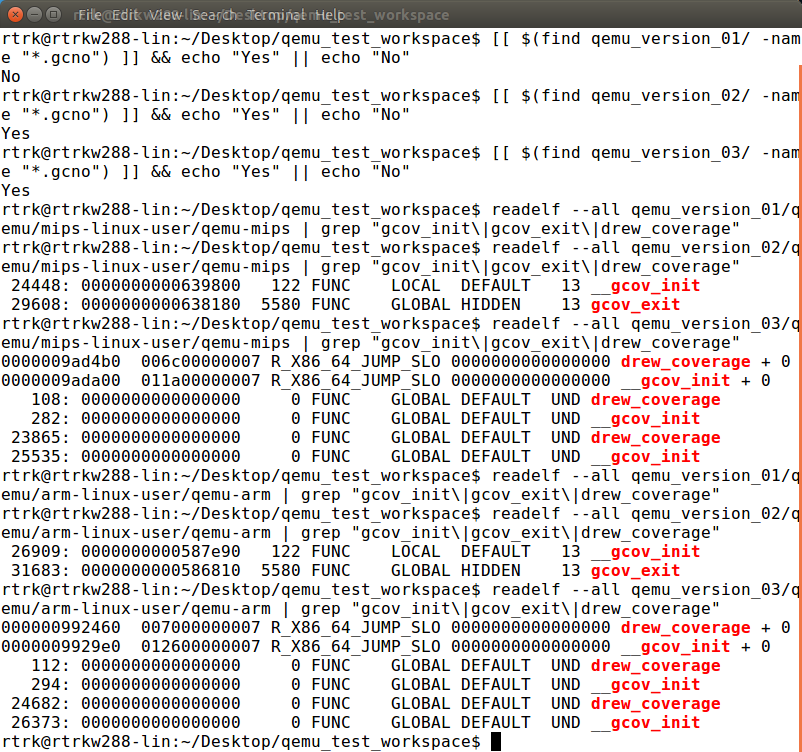
\includegraphics[width=\textwidth]{img/qemu-test-1-ng.png}
  \caption{Testiranje nad projektom \strano{QEMU} - Korak 1}
  \label{fig:qemu-test-1}
\end{figure} 

U okviru drugog koraka, sprovedena je ocena memorijske zahtevnosti. U tabeli \ref{tabela} prikazana je veličina celokupnog projekta, kao i nekoliko pojedinačnih programa unutar projekta, za sve tri verzije. Veličina je prikazana u bajtovima, kao i u obliku procenta regularne veličine. Može se primetiti da se korišćenjem dinamičke biblioteke ostvaruje ušteda od aproksimativno 1\% ukupne veličine.

\begin{table}
\caption{Tabele sa kvantitativnim podacima ocene memorije}
\label{tabela}
\begin{tabular}{ |p{3.35cm}|p{3.2cm}|p{3.2cm}|p{3.2cm}|}
 \hline
 Veličina izražena u bajtovima & \strano{qemu\_version\_01} & \strano{qemu\_version\_02}	& \strano{qemu\_version\_03} \\
 \hline
 qemu-mips & 10556108 & 15203379  & 13598393 \\
 \hline
 qemu-arm & 10700765 & 14960036 & 13917673 \\
 \hline
 qemu-img& 6059717 & 8668398 & 8655375 \\
 \hline
  qemu-system-mips & 34744091 & 47895829 & 46295066 \\
 \hline
  qemu-system-arm & 40898483 & 55292999 & 54251070 \\
 \hline
  qemu/ & 2457828029 & 3727564073 & 3697548246 \\
 \hline
\end{tabular}

\vspace{1em}

\begin{tabular}{ |p{3.35cm}|p{3.2cm}|p{3.2cm}|p{3.2cm}|}
 \hline
 Veličina izražena u procentima & \strano{qemu\_version\_01} & \strano{qemu\_version\_02}	& \strano{qemu\_version\_03} \\
 \hline
 qemu-mips & 100.0000 & 144.0245 & 128.8201 \\
 \hline
 qemu-arm & 100.0000 & 139.8034 & 130.0624 \\
 \hline
qemu-img & 100.0000 & 143.0496 & 142.8346 \\
 \hline
  qemu-system-mips & 100.0000 & 137.8532 & 133.2459 \\
 \hline
  qemu-system-arm & 100.0000 & 135.1957 & 132.6481 \\
 \hline
  qemu/ & 100.0000 & 151.6609 & 150.4397 \\
 \hline
\end{tabular}

\end{table}

Treći korak testiranja obuhvata pokretanje svih šest programa u šest različitih terminala, sa ciljem lakšeg i boljeg poređenja.  Za pokretanje \strano{QEMU} emulatora u koje je linkovana dinamička biblioteka \strano{libcoverage}, preduslov je predstavljalo modifikovanje okruženja. Na vrednost promenljive \strano{LD\_LIBRARY\_PATH} se nadovezuje dodatno putanja do biblioteke \strano{libcoverage}. Prikaz trećeg koraka, za program \strano{qemu-mips} je dat na slici \ref{fig:qemu-test-34}.


\begin{figure}[!ht]
  \centering
  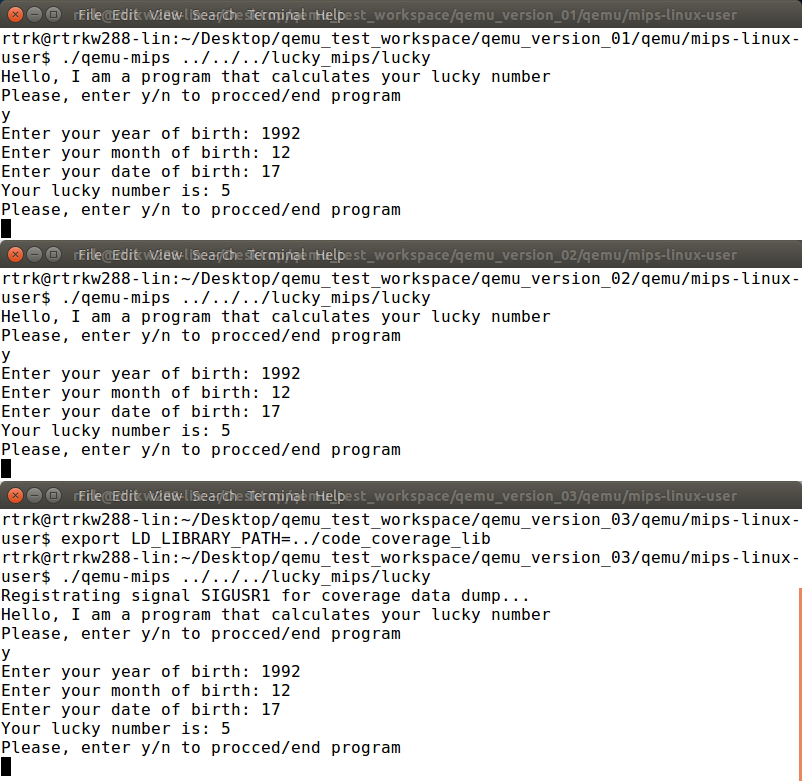
\includegraphics[width=\textwidth]{img/qemu-test-23-ng.png}
  \caption{Testiranje nad projektom \strano{QEMU} - Koraci 3 i 4}
  \label{fig:qemu-test-34}
\end{figure} 

Za spovođenje četvrtog koraka testiranja, koristiće se redukovani slučaj upotrebe programa \strano{lucky} iz prethodne sekcije, sa samo jednim odabirom opcije: y. Na osnovu rezultata ovog koraka, koji su u slučaju programa \strano{qemu-mips} prikazani na slici na \ref{fig:qemu-test-34}, može se zaključiti da instrumentalizacija i prikupljanje podataka ne remete regularan rad emulatora. Time je potvrđena ispravnost korišćenja biblioteke \strano{libcverage} u realnim primenama. 

Procedura narednog koraka se razlikuje u zavisnosti od verzije. Izvršavanje neinstrumentalizovanih programa, više nije neophodno, te se prekidaju odabirom opcije: n. Programi čije podatke iz izvršavanja prikuplja standardna biblioteka \strano{libgcov} se takođe prekidaju na isti način. Statička biblioteka \strano{libgcov} će automatski obaviti funkconalnost kreiranja fajlova \strano{gcda} kao poslednju instrukciju. Pozivom alata \strano{gcov}, za svaki fajl izvornog koda, generišu se dva tipa izveštaja, čije se prisustvo i nepraznost uzimaju za potvrdu uspešnosti ovog koraka testiranja. Validacija je deo procedure narednog koraka. 

Programi treće verzije se ne prekidaju do kraja testiranja. Pokreću se dve instance programa \strano{messanger}, zadužene za prijem signala \strano{SIGUSR1} i prosleđivanje odgovarajuće poruke preostalim aktivnim emulatorima. Unutar interfejsa \strano{code\_coverage\_viewer}, odabira se radni direktorijum: \\ \strano{test\_workspace/qemu\_version\_03/qemu/} i ime programa: \strano{messanger}. Klikom na dugme: \strano{Dump coverage data} kreiraju se fajlovi sa podacima iz dotadašnjeg izvršavanja. Klik na ugme: \strano{Generate gcov and fun files} inicira kreiranje izveštaja, čija se imena mogu videti u drolikoj komponenti grafičkog korisničkog interfejsa, a sadržaj, nakon selektovanja, u desnom polju. Prikaz terminala i ,\strano{code\_coverage\_viewer}-a za oba programa, nakon ovog koraka dat je na slici \ref{fig:qemu-test-5}

\begin{figure}[!ht]
  \centering
  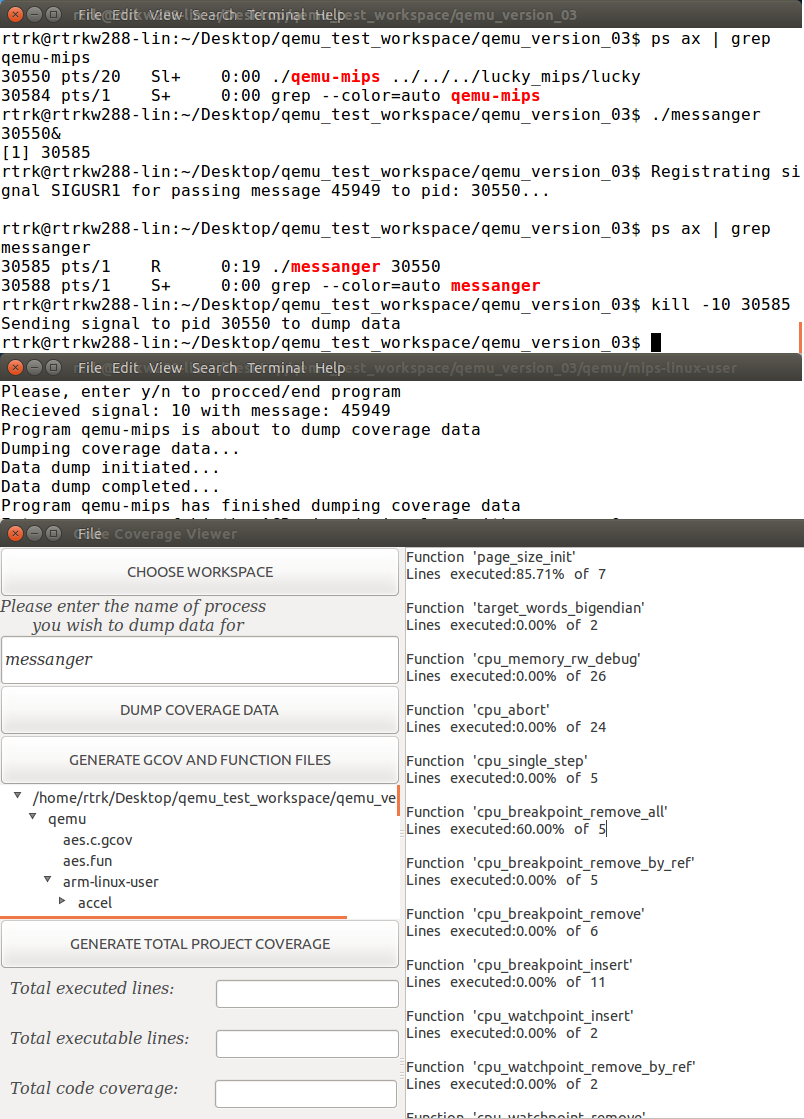
\includegraphics[width=0.97\textwidth]{img/qemu-test-5-ng.png}
  \caption{Testiranje nad projektom \strano{QEMU} - Korak 5c}
  \label{fig:qemu-test-5}
\end{figure} 


Šesta i poslednja faza testiranja predstavlja analizu dobijenih rezultata u cilju njihove validacije. Sastoji se poređenja ispisa na standardni izlaz sa očekivanim, pri čemu se potvrđuje ispravnost instrumentalizacije kao procesa koji ne utiče na rad programa, i  poređenja izveštaja pri čemu se validira ispravnost instrumentalizacije kao procesa koji pruža tačne i precizne informacije. 

Na slici \ref{fig:qemu-test-6a}. je dat prikaz ispisa svih šest programa nakon sprovedenog celokupnog slučaja upotrebe. Očekivano poklapanje ispisa koji vodi poreklo iz inicijalnog dela je potvrđeno, stoga je prvi kriterijum validacije ispisa zadovoljen. Pristustvo oproštajne poruke \strano{Goodbye} u ispisima terminiranih programa, kao i poruke o prikupljanju podataka
potvrđuju ispunjenost preostalih kriterijuma validacije ispisa.

Validacija samih vrednosti podataka o pokrivenosti je sprovedena nad funkcijom: \kod{host\_signal\_handler}, za koju se te vrednosti mogu i statički izračunati, analizom koda i plana testiranja. Programima verzije čiji su instrumentalizacioni simboli razrešeni statičkom binliotekom \strano{libgcov}, nije poslat nijedan signal tokom testiranja. Stoga je očekivana vrednost pokrivenosti funkcije koja odgovara na njih jednaka nuli. Na listingu \ref{qemu-test-6b-1} su prikazani delovi izveštaja: \strano{signal.c.gcov}, koji sadrže podatke o kvantitetu izvršavanja linija koda funkcije: \kod{host\_signal\_handler}. Može se primetiti da nijedna linija koda nije označena kao izvršena. Niska \kod{\#\#\#\#\#} pored linije sa nazivom i argumentima funkcije potvrđuje da se funkcija nije čak ni dlimično izvršavala, odnosno ispunjenje prvog kriterijuma validnosti izveštaja. Programima čije podatke prikuplja biblioteka \strano{libcoverage} je poslat tačno po jedan signal: \strano{SIGUSR1} sa porukom 45949. Na osnovu toga, može se zaključiti da se funkcija \kod{host\_signal\_handler} izvršavala tačno jednom po programu, tokom koji je uslovljen tom kombinacijom. Pozivom funkcije \kod{coverage\_handler}, podaci se prikupljaju iz instrumentalizacionih struktura i beleže. Nakon kreiranja fajlova \strano{gcda}, izvršavanje funkcije \kod{host\_signal\_handler} se nastavlja, s tim što zbog jedinstvenog preseka stanja, podaci o daljem radu programa neće biti zabeleženi. 

\begin{figure}[!ht]
  \centering
  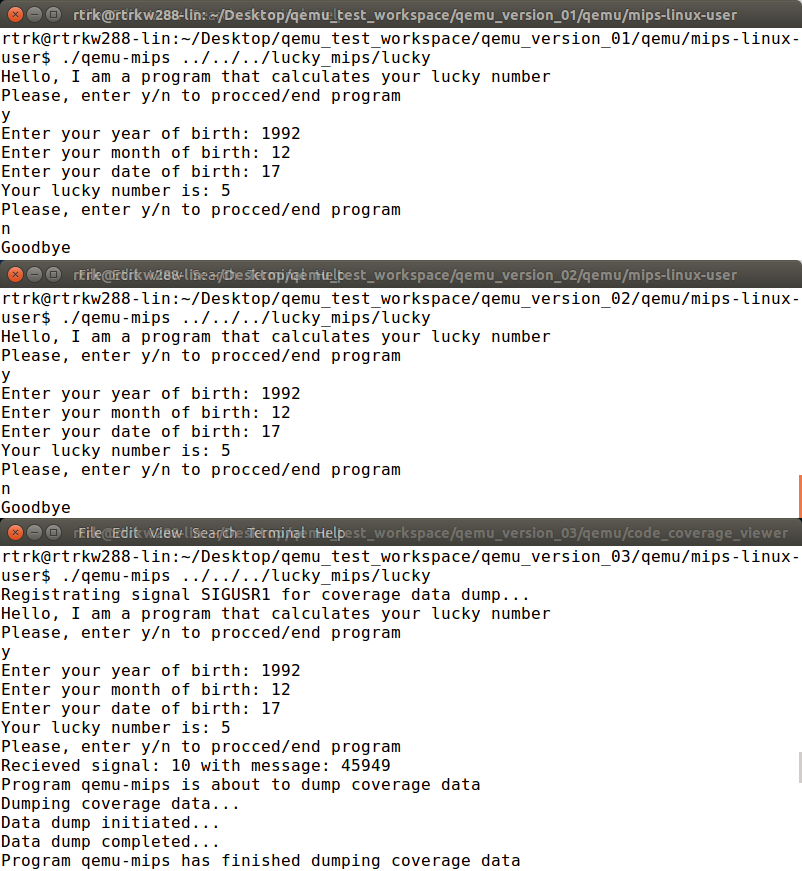
\includegraphics[width=\textwidth]{img/qemu-test-6a-ng.png}
  \caption{Testiranje nad projektom \strano{QEMU} - Korak 6a}
  \label{fig:qemu-test-6a}
\end{figure} 

\newpage

Na listingu \ref{qemu-test-6b-1} su prikazani delovi izveštaja: \strano{signal.c.gcov}, koji sadrže podatke o kvantitetu izvršavanja linija koda funkcije: \kod{host\_signal\_handler}.
Može se primetiti da nijedna linija koda nije označena kao izvršena. Niska \kod{\#\#\#\#\#} pored linije sa nazivom i argumentima funkcije potvrđuje da se funkcija nije čak ni dlimično izvršavala, odnosno ispunjenje prvog kriterijuma validnosti izveštaja. Programima čije podatke prikuplja biblioteka \strano{libcoverage} je poslat tačno po jedan signal: \strano{SIGUSR1} sa porukom 45949. Na osnovu toga, može se zaključiti da se funkcija \kod{host\_signal\_handler} izvršavala tačno jednom po programu, tokom koji je uslovljen tom kombinacijom. Pozivom funkcije \kod{coverage\_handler}, podaci se prikupljaju iz instrumentalizacionih struktura i beleže. Nakon kreiranja fajlova \strano{gcda}, izvršavanje funkcije \kod{host\_signal\_handler} se nastavlja, s tim što zbog jedinstvenog preseka stanja, podaci o daljem radu programa neće biti zabeleženi. 
\\

\begin{lstlisting}[caption={Testiranje nad projektom \strano{QEMU} - Korak 6b bez izmena} ,frame=single, label=qemu-test-6b-1]
    #####:  645:static void host_signal_handler(int host_signum,
        -:  646:                        siginfo_t *info, void *puc)
        -:  647:{
    #####:  648:    CPUArchState *env = thread_cpu->env_ptr;
    #####:  649:    CPUState *cpu = ENV_GET_CPU(env);
    #####:  650:    TaskState *ts = cpu->opaque;
        -:  651:
        -:  652:    int sig;
        -:  653:    target_siginfo_t tinfo;
    #####:  654:    ucontext_t *uc = puc;
        -:  655:    struct emulated_sigtable *k;
        -:  656:
        -:  657:    /* the CPU emulator uses some host signals to detect exceptions,
        -:  658:       we forward to it some signals */
    #####:  659:    if ((host_signum == SIGSEGV || host_signum == SIGBUS)
    #####:  660:        && info->si_code > 0) {
    #####:  661:        if (cpu_signal_handler(host_signum, info, puc))
    #####:  662:            return;
        -:  663:    }
        -:  664:
        -:  665:    /* get target signal number */
    #####:  666:    sig = host_to_target_signal(host_signum);
\end{lstlisting}

Na listingu \ref{qemu-test-6b-2} su prikazani delovi izveštaja:
\strano{signal.c.gcov} koji sadrže podatke o kvantitetu izvršavanja linija koda funkcije: \kod{host\_signal\_handler}. Linije koda, zaključno sa onom koja se odnosi na poziv funkcije \kod{coverage\_handler}, koje pripadaju toku izvršavanja karakrerističnom za prijem signala \strano{SIGUSR1} sa porukom  45949, su označene kao jedinstveno izvršene. Sve linije koda koje se izvršavaju nakon poziva funkcije: \kod{coverage\_handler}, odnosno kreiranja fajlova \strano{gcda} su označene ka neizvršene. Dobijeni rezultati su u skladu sa očekivanjima i zahtevima drugog kriterijuma validacije izveštaja. Stoga se i ovaj kriterijum može označiti kao ispunjen. 

\newpage

\begin{lstlisting}[caption={Testiranje nad projektom \strano{QEMU} - Korak 6b sa izmenama} ,frame=single, label=qemu-test-6b-2]
        1:  649:static void host_signal_handler(int host_signum,
        -:  650:                        siginfo_t *info, void *puc)
        -:  651:{
        1:  652:    CPUArchState *env = thread_cpu->env_ptr;
        1:  653:    CPUState *cpu = ENV_GET_CPU(env);
        1:  654:    TaskState *ts = cpu->opaque;
        -:  655:
        -:  656:    int sig;
        -:  657:    target_siginfo_t tinfo;
        1:  658:    ucontext_t *uc = puc;
        -:  659:    struct emulated_sigtable *k;
        -:  660:
        -:  661:    /* the CPU emulator uses some host signals to detect exceptions,
        -:  662:       we forward to it some signals */
        1:  663:    if ((host_signum == SIGSEGV || host_signum == SIGBUS)
    #####:  664:        && info->si_code > 0) {
    #####:  665:        if (cpu_signal_handler(host_signum, info, puc))
    #####:  666:            return;
        -:  667:    }
        -:  668:
        -:  669:    /* get target signal number */
        1:  670:    sig = host_to_target_signal(host_signum);
        1:  671:    if (sig < 1 || sig > TARGET_NSIG)
    #####:  672:        return;
        -:  673:
        -:  674:
        1:  675:     int message_int = info->si_value.sival_int;
        1:  676:     printf("Recieved signal: %d with message: %d\n",host_signum, message_int);
        -:  677:     //Checking if signal and message corespond to predefind coverage dumping comunication
        1:  678:     if (host_signum == SIGUSR1 && message_int == 45949){
        -:  679:#ifdef RUNTIME_GCOV
        -:  680:       // informing about begining of coverage dump procedure and invoking coverage handler that will do the dumping
        1:  681:        printf("Program %s is about to dump coverage data\n", program_invocation_short_name);
        1:  682:        coverage_handler(host_signum);
        -:  683:       //Informing about end of coverage dump procedure
    #####:  684:        printf("Program %s has finished dumping coverage data\n", program_invocation_short_name);
        -:  685:        // reseting value of message since it is alredy being processed.
    #####:  686:        info->si_value.sival_int = 0;
\end{lstlisting}

Generisanje ukupne pokrivenosti projekta će biti sprovedeno na isti način kao i u okviru testiranja nad programom \strano{lucky} u prethodnoj sekciji.Jednostavnim prebrajanjem linija koje su u izveštajima označene kao izvršene/izvršne, i računanjem količnika ta dva broja, dobijaju jednake vrednosti kao one koje su generisane novim interfejsom i prikazane na slici \ref{fig:qemu-test-6c}

\begin{figure}[!ht]
  \centering
  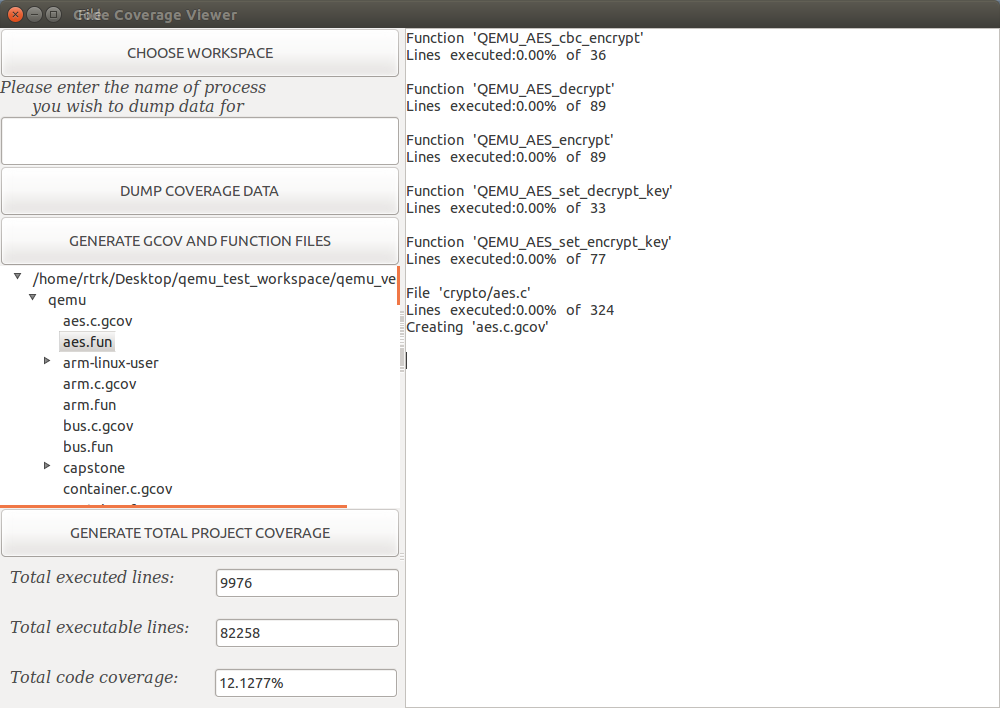
\includegraphics[width=\textwidth]{img/qemu-test-6c-ng.png}
  \caption{Testiranje nad projektom \strano{QEMU} - Korak 6c}
  \label{fig:qemu-test-6c}
\end{figure} 

Na osnovu uspešnih rezultata svih koraka predviđenog plana za testiranje, testiranje se može smatrati uspešnim.


% ------------------------------------------------------------------------------
\chapter{Zaključak}
% ------------------------------------------------------------------------------

U okviru ovog rada proučavana je analiza programa, njene vrste i tehnike. Posebno je proučavana tehnika dinamičke analize pod nazivom profajliranje, koja obezbeđuje razne informacije o ponašanju programa, među kojima je i pokrivenost (stepen izvršenosti) koda. Ove informacije predstavljaju važne vodilje procesa testiranja i optimizacije softvera. Definisane su i ukratko objašnjene sve tri faze profajliranja: instrumentalizacija, odnosno ubrizgavanje koda za praćenje izvršavanja, prikupljanje metapodataka o izvršavanju programa i njihovo prezentovanje. Detaljno su ispitivane implementacija i mogućnosti poslednje dve faze, kao i prostor za njihovo unapređenje, u okviru različitih programskih prevodioca: \strano{ICC}, \strano{Clang} i \strano{GCC}.

Svi proizvodi kompanije \strano{Intel} su zaštićeni komercijalnim licencama, zbog čega je istraživanje podrške sadržane u okviru programskog prevodioca \strano{ICC} ograničeno na analizu javno dostupne dokumentacije u cilju oblikovanja ideje za ovaj rad. Najviši stepen podrške, koji obuhvata i mogućnost informisanja o pokrivenosti koda u toku izvršavanja, ugrađen je u podprojekat \strano{compiler-rt} projekta \strano{LLVM}. Međutim, odlikuju ga loše perfomanse, pre svega prostorna složenost, a optimizacija do zadovoljavajućeg nivoa bi iziskivala krupne algoritamske promene. Zbog toga je i ova implementacija odabrana samo za idejnu vodilju. Podaci koji opisuju izvršavanje programa prevedenih \strano{GCC}-om dostupni su tek nakon okončanja rada programa, ali proces prikupljanja karakteriše veoma pouzdan algoritam i dobre performanse. 

Značaj obavljanja celokupnog procesa profajliranja u toku izvršavanja, naročito se ogleda na softverskim rešenjima, čije je vreme rada veoma dugo, ne mogu se prekidati radi analize, i/ili su podaci dostupni/korisni isključivo u toku izvršavanja. Primer su operativni sistemi, serveri, kao i sistemi za rad u realnom vremenu. Ovakvi sistemi često imaju veoma ograničene memorijske mogućnosti, pa ne mogu koristiti ni profajliranje implementirano u programski prevodilac projekta \strano{LLVM}.
 
Na osnovu analize mogućnosti trenutnih implementacija, kao i potreba koje treba da zadovolji kvalitetno profajliranje, zaključeno je da prevodilac GCC ima najveći potencijal za unapređenje do optimalnog rešenja, ugradnjom podrške za prikupljanje podataka iz izvršavanja u toku rada programa. Analizom \strano{GCC}-ovog alata \strano{gcov}, koji obrađuje i preznentuje ovako prikupljene podatke, ustanovljen je i dodatni prostor za unapređenje treće faze profajliranja u pravcu bolje preglednosti i povišene informativnosti. Neke od karakteristika alata \strano{gcov} koje utiču na smanjenje kvaliteta korisničkog doživljaja su: raspršenost izveštaja po radnom direktorijumu projekta, manjak informacija u izveštaju prilikom korišćenja dodatnih opcija alata, kao i nedostatak informacije o pokrivenosti na nivou projekta.

U okviru ovog rada implementirano je softversko rešenje problema prikupljanja i prezentovanja podataka iz izvršavanja programa u toku njegovog rada. 
Rešenje se sastoji iz \strano{backend} podrške u vidu dinamičke biblioteke \strano{libcoverage}, koja omogućava dostupnost podataka u toku izvršavanja, i \strano{fronend} podrške u vidu grafičkog interfejsa \strano{code\_coverage\_viewer}, koji unapređuje korisnički doživljaj prezentovanja podataka. Nova biblioteka je izgrađena po uzoru na postojeću biblioteku libgcov i u potpunosti pokriva i njene funkcionalnosti. Izgrađena je kao dinamička i nezavisna od prevodioca u cilju postizanja maksimalne fleksibilnosti i performansi. Poziv funkcije za kreiranje binarnih fajlova sa podacima iz izvršavanja, prepušten je vlasniku programa. Ponuđena je i opciona implementacija poziva putem signala. Novi grafički interfejs predstavlja omotač celokupnog procesa prikupljanja i prikaza podataka, sa osnovnom ulogom strukturnije i intuivnnije prezentacije podataka iz izvršavanja. Omogućava generisanje i pregledanje linijskih i funkcijskih izveštaja. Bolja preglednost je postignuta smeštanjem izveštaja u drvo koje odražava strukturu direktorijuma. Informativnost je povišena dodatnim funkcijskim izveštajima, kao i prikazom ukupne statistike. 

Dalji razvoj bi mogao ići u pravcu proširivanja funkcionalnosti na druge prevodioce ili programske jezike, unapređivanja biblioteke ili alata. U cilju unapređenje biblioteke bi se mogla implementirati podrška za višestruko pozivanje funkcije za prikupljanje u toku jednog izvršavanja, koje trenutno nije dozvoljeno zbog opasnosti višestrukog sumiranja istih podataka. Sa druge strane, dalji razvoj alata bi mogao obuhvatati dodavanje novih vrsta izveštaja ili novih vrsta sumarnih podataka, poput na primer sortirane statistike po svim modulima.


% ------------------------------------------------------------------------------
% Literatura
% ------------------------------------------------------------------------------
\literatura

% ==============================================================================
% Završni deo teze i prilozi
\backmatter
% ==============================================================================

% ------------------------------------------------------------------------------
% Biografija kandidata
\begin{biografija}
  \textbf{Marina Nikolić} (\emph{Sombor,
    17. decembar 1992. }) je ... 
\end{biografija}
% ------------------------------------------------------------------------------

\end{document}
